\documentclass[a4paper,11pt]{report}
\usepackage{a4wide}
\usepackage[frenchb]{babel}
\usepackage[utf8]{inputenc}
\usepackage[T1]{fontenc}
\usepackage{geometry}
\usepackage{graphicx}
\usepackage{fancybox}
\usepackage[pdftex]{hyperref} %Liens dans table de matieres
\usepackage{fancyhdr}
\usepackage{geometry}
\usepackage{url}
\usepackage{multicol}

\usepackage{pstricks}

%\geometry{scale=0.75, nohead}


\newcommand*{\enConstruction}[1]{
	\vspace*{.1cm}
	\doublebox{
	    \begin{minipage}{.9\linewidth}
	      --- #1 \\ 
	    \end{minipage}
	}
}

\newcommand*{\precision}[1]{
	\vspace*{.1cm}
	\fbox{
		\begin{minipage}{.9\linewidth}
			#1 
		\end{minipage}
  	}\\
}

% Title Page
\title{
	
\includegraphics[scale=.2]{logofds.eps}\\
	\vspace*{1cm}
	TER FMIN200 \\ 
	-- \\
	Développement d'un jeu de type Bomberman en réseau sous Android et iOS
}

\author{BONVILA Olivier \and COUSEIN Kilian \and PITIOT Ludovic \and TARDIEU Benjamin}

\date{}

\begin{document}
\maketitle

\thanks{

  Nous tenons à remercier 

}

\tableofcontents


\chapter{Introduction}

	Nous sommes amenés, dans le cadre de notre première année en master informatique à la faculté des Sciences de Montpellier, à travailler sur l’élaboration complète d’un projet, de son analyse à la conception puis à sa programmation. Tout au long de ce deuxième semestre, le projet nous permet de comprendre quelles sont les phases de développement d’un projet et comment celui-ci doit être conduit. Nous pouvons par ailleurs mesurer notre capacité à réagir face à des problèmes en nous impliquant dans ce projet. Le projet que nous avons choisi constiste à réaliser sur deux \glspl{os} de téléphone différents un jeu de type Bomberman.

Ce projet nous permet de mettre en application l'enseignement que nous avons acquis tout au long de ce semestre. Ce dernier étant spécialisé pour chaque étudiant, il nous a permis de travailler en collaboration avec des personnes aux capacités différentes et d'ainsi mettre nos connaissances en commun. Mais il permet aussi de se faire une idée du travail demandé dans le monde des entreprises et d'ainsi nous préparer à notre stage que nous devrons réaliser l'an prochain.

Afin de comprendre la démarche que nous avons utilisée pour mener ce projet à son terme, notre rapport se compose de cinq grandes parties : 

Tout d'abord, dans une première partie, nous présentons le cadre général de notre projet ainsi que le jeu que nous avons développé. Ensuite, dans une seconde, partie nous verrons comment nous nous sommes orgnanisé pour mener à bien la conduite de notre projet. Puis dans une troisième partie, nous présenterons le travail d'analyse que nous avons effectué pour pouvoir ensuite, dans une quatrième partie, expliquer le developpement du projet. Enfin, nous finirons en expliquant l'implémentation de la réutilisabilité dans le code pour pouvoir ensuite finir sur la conclusion.

\chapter{Présentation}

	En tant que première année de master, nous avons dû developper un projet tout au long de ce semestre. Chaque année une liste de projets est présentée aux étudiants. Tous les étudiants doivent former des groupes pour développer l'un des projets choisi. Puis ces derniers sont associés à un tuteur. Etant donné que nous voulions développer notre propre projet, nous avons formé un groupe de quatre personnes : Olivier BONVILA, Kilian COUSEIN, Ludovic PITIOT et Benjamin TARDIEU. Ensuite, pour pouvoir valider notre sujet, nous avons dû trouver un tuteur voulant bien s'occuper de notre tutelle. Mr Laurent Deruelle a gentiment accepté de s'occuper de notre groupe, mais pour que ce dernier soit entièrement validé, des modifications du sujet ont été nécessaires.

\section{Projet}	
	
 Etant donné que nous voulions principalement créer une application
 \gls{iphone}, nous avons demandé à développer notre propre projet. Un jeu de
 type Bomberman. Mais ce dernier a dû subir des modifications pour être
 approuvé. Nous avons donc dû développer le jeu sous \gls{iphone} et sous
 \gls{android}. Le but étant de comparer la différence de développement entre
 les deux types de téléphones et de développer des fonctionnalités en rapport
 avec les parcours d'enseignement que nous avons choisi ce semestre.\\
	
	
Pour pouvoir rapprocher le développement de cette application à notre parcours
d'enseignement. Nous avons choisi de développer un mode solitaire qui permettra
de jouer contre une ou plusieurs intelligences artificelles qui est en rapport
avec le cursus \gls{i2a} qui nous est enseigné. Ensuite, pour ce qui est du
parcours \gls{casar}, nous avons décidé d'implémenter un mode multijoueur qui
permettra à plusieurs joueurs connectés en \gls{wi-fi} de jouer en réseau grâce
à un serveur qui combinera un serveur d'applications et un serveur web. Pour ce qui est de la conception de toute la structure du programme nous avons mis en application nos connaissances apprises dans le parcours \gls{gl}. Puis pour ce qui est du parcours \gls{diweb}, la partie serveur permettra de palier à
l'enseignement de ce dernier. 
	


\section{Plate-formes de développement}
	\subsection{Android}
	\begin{itemize}
		\item{De qui ?}
		\item{Langage}
		\item{PC}
		\item{SDK - (le contenu)}
	\end{itemize}

\subsection{iOS}
	\begin{itemize}
		\item{De qui ?}
		\item{Langage}
		\item{Mac}
		\item{SDK - (le contenu)}
	\end{itemize}
	
\section{Organisation}
			Les gestionnaires de versions comme leur nom l'indique, permettent d'avoir à
		porté de main toutes les versions qu'il y a eu d'un fichier depuis sa
		création, cela permet donc de pouvoir revenir en arrière si une erreur a été commise.
		De plus grâce à cela, notre projet reste cohérent dans le sens où pour pouvoir
		être mis à jour, il faut à tout prit avoir modifié un fichier à partir de la
		dernière version de celui-ci.
		
		Dernier avantage d'avoir utilisé un gestionnaire de version et qu'il est
		hébérgé sur le net et donc chaque membre de l'équipe peut y accéder où qu'il
		soit. 
		
		De plus \emph{\gls{google_code}} met aussi à disposition de ses utilisateurs des \glspl{wiki}.
		Un \gls{wiki} est un site Web dont les pages sont modifiables par les développeurs
		afin de permettre l'écriture et l'illustration collaboratives des documents numériques qu'il contient.
		
		Malgré de nombreuses réunions quotidiennes afin d'organiser au mieux le développement de cette application dont nous ignorons
		tout à nos début. Nous avons utilisé le \gls{wiki} qui nous a été fourni afin de partager au mieux
		les découvertes que nous faisions au fur et à mesure ainsi que les articles qui nous semblaient interressants.
		
		En ce qui concerne la répartition du travail, celle-ci s'est faite naturellement car
		seulement la moitiée du groupe possédait de quoi développer sous \gls{ios}, de là nous avons
		donc créé deux équipes une sous \gls{android} et l'autre sous \gls{ios}.
		
		
		DIAGRAMME DE GANT

	
	
\chapter{Analyse}
	\begin{itemize}
		\item{Introduction}
	\end{itemize}
	
	\section{Cahier des charges}
	\subsection{Menus}
		
	Les menus se doivent d'être clairs et de rendre l'utilisation de
	l'application aisée. Il s'agit d'un jeu ne demandant aucune compétence
	particulière. Il va donc toucher un public large et doit pouvoir convenir à
	tout utilisateur. Cela passe d'abord par une navigation intuitive dans les
	menus.
		
\subsection{Jeu}
		
	Le jeu est la partie la plus importante du projet. 
	Il se decompose en trois éléments : le model, la vue et le controlleur. 
	Le modèle est composé du moteur physique, du moteur de rendu ainsi que de la
	hierarchie de classes permettant de representer l'ensemble des objets du jeu. 
	La vue quant à elle est composée d'objets graphiques simples (bouttons, images, ... ) 
	et d'une partie reprèsentant le jeu. Elle se doit d'être ergonomique et de permettre
	à l'utilisateur de pouvoir jouer très simplement. Le controlleur fait
	le lien entre les actions de l'utilisateur sur le modèle. Cette décomposition aura
	l'avantage de pouvoir modifier facilement le modèle et/ou la vue.
		
	L'application doit aussi pouvoir changer de langue, avec comme langues initiales le francais et l'anglais.
	Elle doit permettre à l'utilisateur de jouer à des parties solitaires ou multijoueur. 
	Ce dernier possèdera un compte hors ligne et en ligne.		
	Le premier servira à personnaliser son profil comme par exemple pour modifier
	la couleur du joueur, changer son pseudo ou encore à enregistrer les informations
	et les preferences de connexion sur une base de données locale,
	mais également les scores du joueurs (nombre de parties gagnées ou perdus).
	
	Dans le jeu l'utilisateur peut créer différents comptes hors lignes en cas de partage du télephone
	avec un ami ou un membre de sa famille, pour pouvoir garder en mémoire ses scores et ses préferences.		
	Le compte en ligne quant à lui servira seulement à établir une connexion avec le serveur distant pour pouvoir jouer en multijoueur.		
	Un menu d'aide doit apparaitre afin d'aider le joueur à comprendre le but du jeu et comment jouer. 
	Ce dernier est simple et très explicite étant donné la large tranche d'âge des utilisateurs que vise cette application.		
	Ensuite un éditeur de carte permettra aux utilisateurs de créer un large choix de cartes
	grâce à une multitude de différents objets qui les composeront. Ces dernieres pourront être seulement utilisées en mode solitaire.
	Pour les parties solitaires une intelligence artificielle avec trois niveaux de difficulté 
	devra permettre à un joueur débutant, intermédiaire ou confirmé de jouer comme bon lui semble pour pouvoir améliorer sa maniere de jouer.
	
\subsection{Serveur}
	
	Le serveur représente la partie réseau de notre projet et rend fonctionnel le jeu entre plusieurs téléphones via des parties multijoueur (qu'ils soient de type
	\gls{ios} ou \gls{android}). Autrement dit il servira d'hebergeur pour les parties et
	il se chargera de l'intéraction entre les joueurs, via leur mobile.
	
	Il devra être capable d'enregistrer des inscriptions de nouveaux joueurs, avec
	vérification afin qu'il n'y ait pas de doublon. Ces derniers seront inscrits dans 
	la base de données du serveur. Les joueurs devraient ainsi
	pouvoir se connecter en utilisant le couple nom d'utilisateur/mot de passe,
	préalablement choisi. Suite à cela les utilisateurs seront à même de lister
	les parties en cours, ils pourront choisir de créer des parties ou de les rejoindres.
	
\section{Modélisation}
	\subsection{Général}
	Le fait de développer des applications \gls{ios} et \gls{android}, nous a 
	imposé le choix du langage.
	En effet pour développer des applications \gls{iphone}, il faut utiliser 
	le langage \gls{objective-c}.
	Pour les applications \gls{android} c'est le langage \gls{java} qui est 
	utilisé.
	
	Ces deux langages ont une syntaxe complétement différente mais sont quand 
	même très proches car ce sont des langages orientés objets.
	Grâce à cela nous avons pu mettre au point une modélisation générale de 
	l'application que nous avons ensuite adapté à chaque langage.\\
			
	Nous avons décidé de développer en anglais car premièrement c'est la langue
	la plus utilisée dans le monde de la programmation et deuxièmement car la 
	syntaxe des langages est toujours en anglais.
	Cela permettra à n'importe quel utilisateur de n'importe quelle nationalité 
	de comprendre le code de l'application.\\
			
	La documentation des deux applications est également en anglais.
	Cette documentation permettra à tout utilisateur de comprendre le 
	fonctionnement de celle-ci, que ce soit sur \gls{iphone} ou \gls{android}.
	
	Chacune d'elles est au format \gls{html} et sera donc directement visible 
	grâce à un navigateur Web.\\
			
	Pour ce qui est de la modélisation globale du projet, nous avons choisi de 
	développer les deux applications selon le modèle \gls{mvc}.
	Ce dernier est une architecture et une méthode de conception qui organise 
	l'\gls{ihm} d'une application logicielle. 
			
	Le modèle représente le comportement de l'application : traitements des
	 données, interactions avec la base de données, etc.
	Il décrit et contient les données manipulées par l'application, assure 
	la gestion de ces données et garantit leur intégrité.
			
	La vue correspond à l'interface avec laquelle l'utilisateur interagit.
	Sa première tâche est de présenter les résultats renvoyés par le modèle.
	La seconde est de recevoir toutes les actions de l'utilisateur 
	(clic de souris, sélection d'une entrée, boutons, etc).
			
	Le contrôleur prend en charge la gestion des événements de synchronisation 
	pour mettre à jour la vue ou le modèle et les synchroniser.
	Il reçoit tous les événements de l'utilisateur et enclenche les actions 
	à effectuer.
			
	Grâce à cette méthode de conception le code est décomposé en trois parties 
	bien distinctes qui permettent la maintenance et l'amélioration du projet.
	Cela permet aussi d'améliorer chacune des trois parties sans avoir à 
	modifier les deux autres.
	Par exemple de changer de vue et donc avoir des interfaces graphiques différentes.
			
\subsection{Menus}

	Au démarrage de l'application vous arrivez sur un menu d'accueil. Depuis
	celui-ci vous pourrez accéder à l'aide, à la liste des comptes locaux ou à la
	création d'un nouveau compte local.
	
	Ils se divisent en quatre grandes sections.
		
	Premièrement la section de création de parties locales dans laquelle l'utilisateur
	pourra choisir parmi une liste de cartes celle sur laquelle il désire jouer.
	Le réglage de la difficulté des \glspl{bot}, leur nombre et le temps de jeu.
		
	Dans la même catégorie se trouve la section des parties multijoueurs. En
	accédant à celle-ci vous allez pouvoir vous connecter à votre compte
	multijoueur ou le créer s'il n'est pas déjà fait. Vous accèderez ensuite à la liste
	des parties multijoueurs, que vous pourrez rejoindre ou choisir de créer la
	votre. Dans le menu création le principe est proche des parties locales.
		
	Suite à ces deux sections vient ensuite l'éditeur de cartes.
	C'est depuis ce menu que vous créerez une nouvelle map de jeu local ou 
	éditerez l'une d'entre elles.
		
	Enfin vient le menu des options où vous pourrez gérer vos
	préférences sytèmes telles que le volume ou la langue de
	l'application(anglais, français).
	Une sous-section de gestionnaire de profil est aussi présente.
	Une édition de vos comptes locaux, multijoueurs ou même
	vos paramètres de jeu comme la position du menu, sont modifiables depuis ce 
	menu.
	
	\begin{figure}
		\label{activité}
		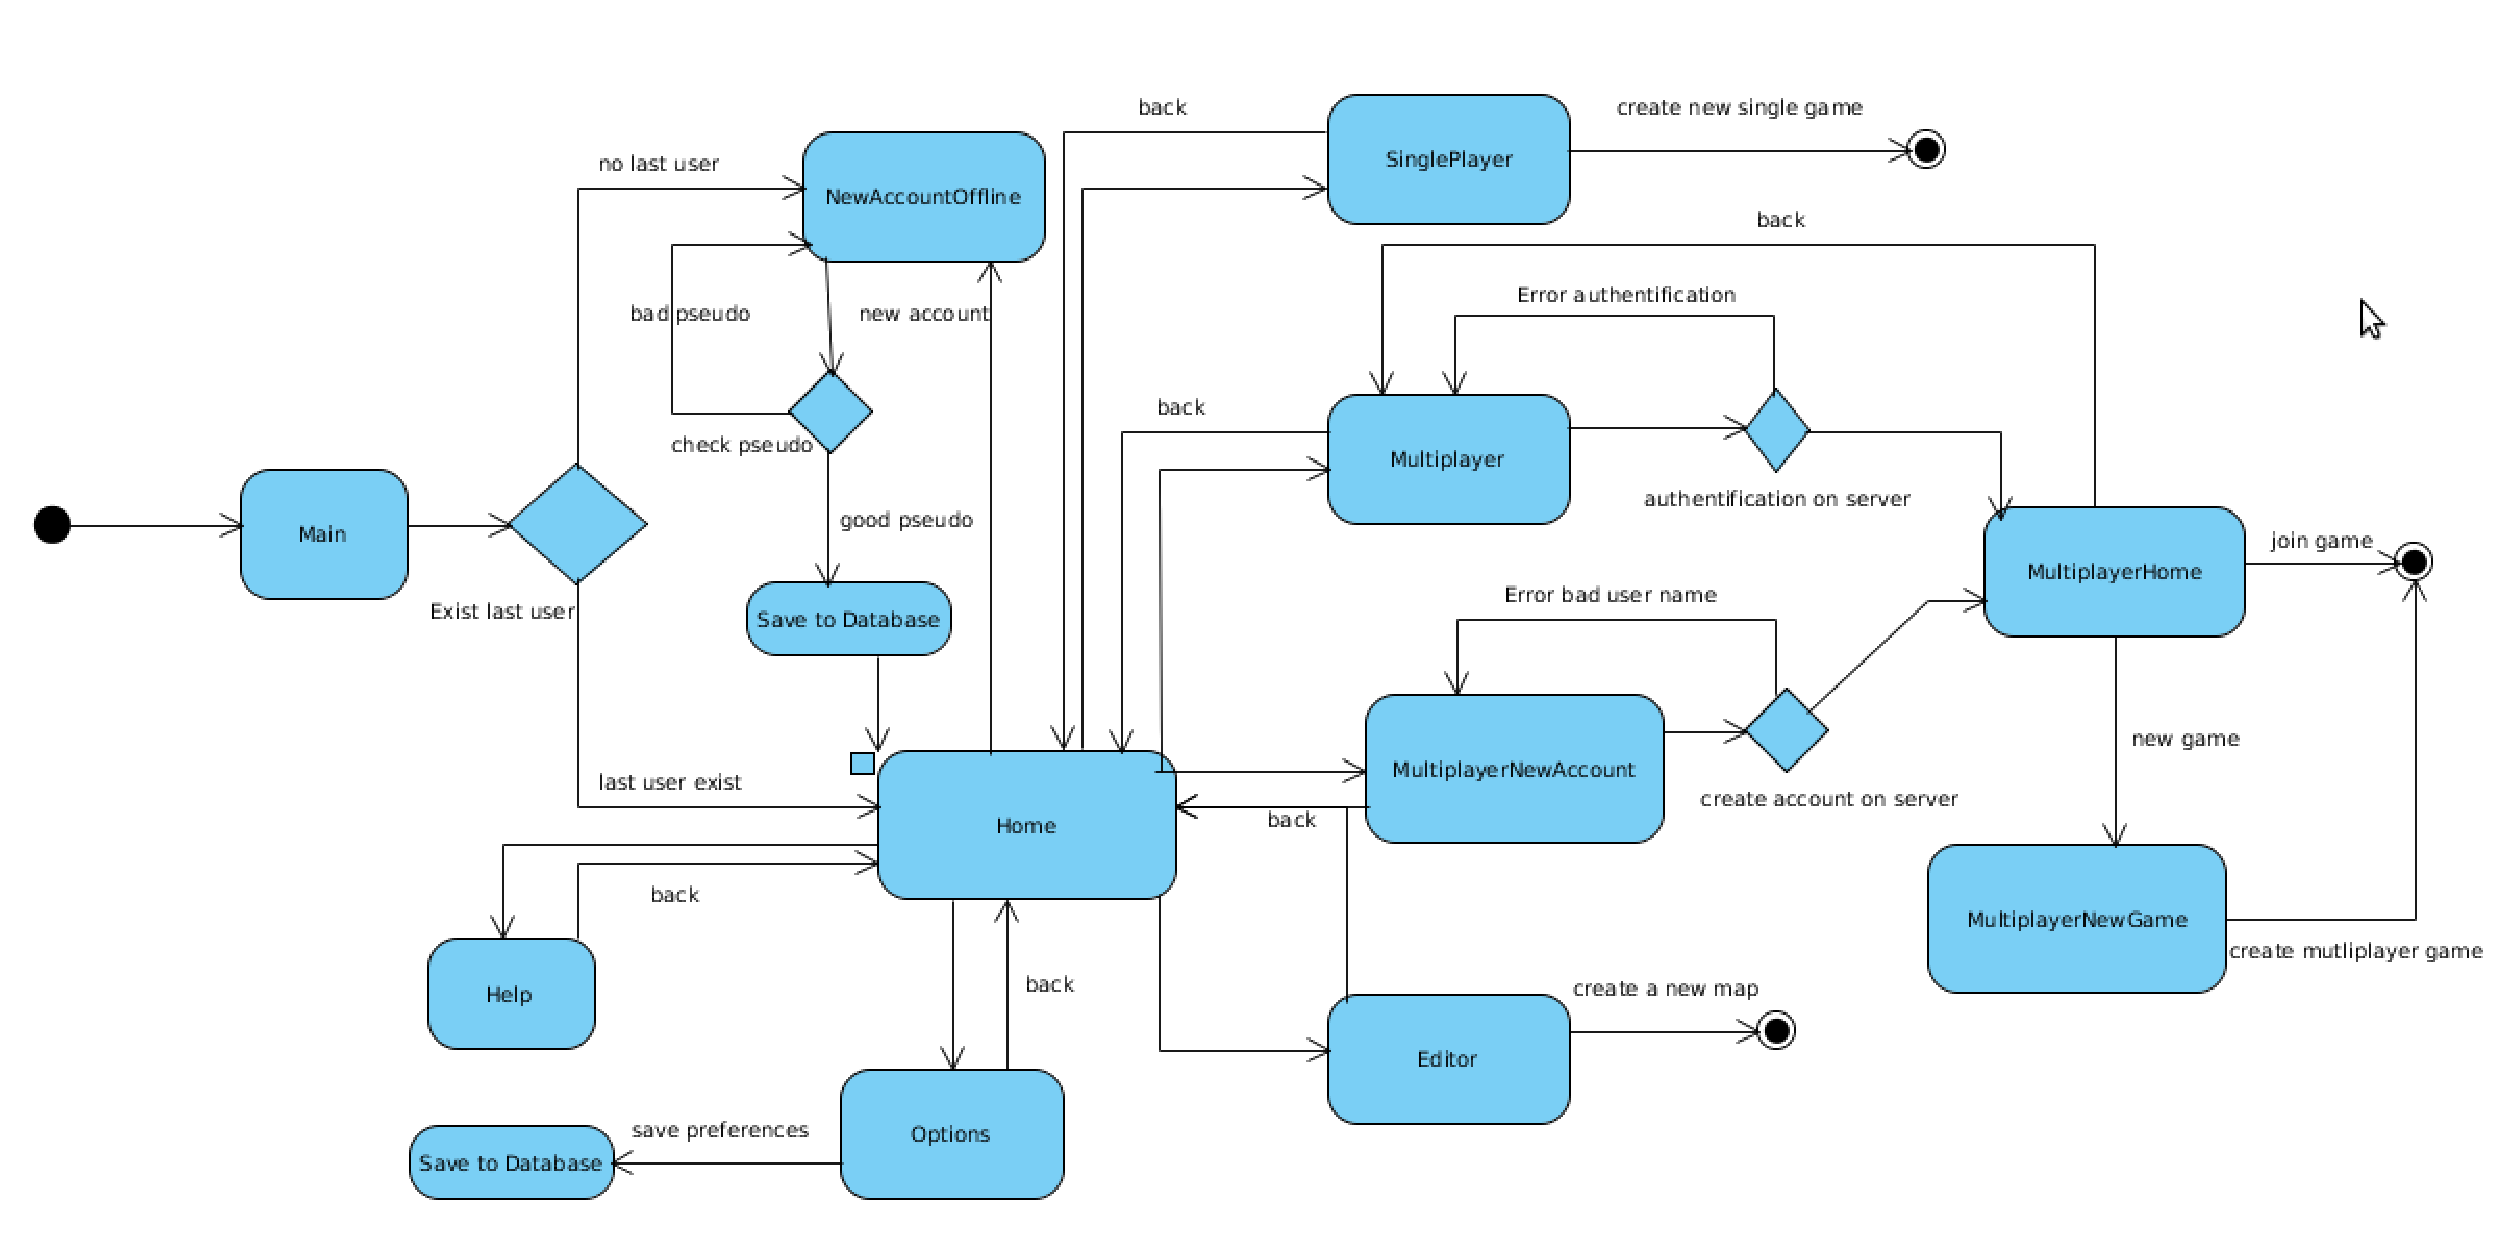
\includegraphics[width=23cm, angle=90]{Analyse/Img/diag_activity.eps}
		\caption{Diagramme d'activité}
	\end{figure}

	\paragraph{Base de données\\}
			
		Une base de données locale a elle aussi été conçue. Cette dernière a pour
		but de stocker plusieurs types de données.
				
		En effet dès lors qu'un compte local est créé sur le téléphone dans la
		table PlayerAccount, il est possible de conserver ses préférences tels 
		que la couleur du joueur, le pseudonyme ou même ses paramètres de connexion multijoueur.
				
		L'application est par ailleurs en mesure de conserver
		les valeurs sonores, la langue et même le dernier utilisateur de
		l'application grâce à un son identifiant qui est clé étrangère dans la table System(attribut lastUser).
				
		De plus l'application sera délivrée avec quelques cartes officielles, mais
		l'utilisateur aura libre droit de créer ses propres cartes de jeu via un
		éditeur. Elles seront alors stockées dans la table Map avec toujours une
		clé étrangère vers l'identifiant de son créateur. \\
		
		\newpage
				
		\begin{figure}
			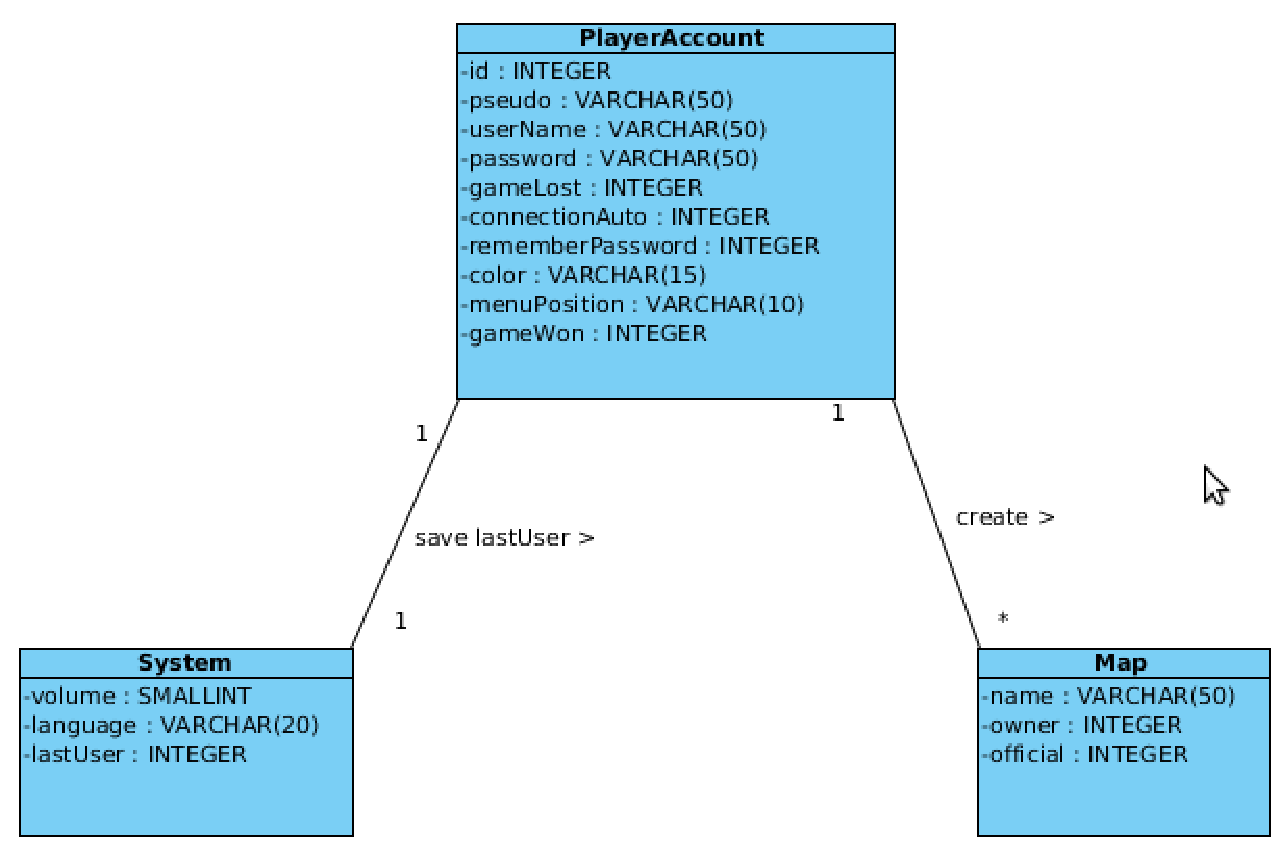
\includegraphics[width=11cm]{./Analyse/Img/menu_bdd.eps}
			\caption{Diagramme de classe Base de données}
		\end{figure}	
	
\subsection{Editeur de carte}	

	L'éditeur de carte est une fonctionnalité qui va permettre à un utilisateur
	 de créer facilement ses propres cartes pour ensuite y jouer dessus contre 
	 l'intelligence artificielle.
	 
	Après avoir réfléchi sur toutes les fonctionnalités que l'éditeur de carte 
	devait remplir, nous avons retenu celles-ci : permettre à l'utilisateur d'en créer une nouvelle,
	 mais aussi de pouvoir charger une ancienne carte 
	précèdemment créée.
	
	Il peut modifier le sol de la carte, ajouter ou supprimer des blocs de 
	la carte et enfin placer les différents points de départ des joueurs sur 
	la carte.
		
	Pour réaliser cette partie de l'application, nous avons aussi utilisé le 
	modèle de conception MVC.

	\subsubsection*{Modèle}
		La partie modèle va contenir toutes les données de l'éditeur de carte. Les cartes sont les principales données qu'il va devoir manipuler. Pour cela nous avons décidé de la réprésenter sous la forme de deux matrices, la première représentant les objets du premier niveau (le sol) et la deuxième la matrice du second niveau (les blocs, les points de départ des joueurs, etc).
			
			
	\subsubsection*{Vue}
		Ensuite, la vue représentera l'interface graphique de notre éditeur de carte. La principale difficulté pour réaliser l'interface graphique était de devoir rentrer toutes les informations nécessaires pour l'éditeur de carte dans un écran de type \gls{smartphone}. Après plusieurs prototypes d'interface, nous avons décidé de séparer l'interface en trois parties. Tout d'abord la plus grande partie, l'affichage de la carte, qui comme étant la principale information à afficher, nous avons essayé de maximiser sa taille. Ensuite un menu à droite permettant au joueur de changer d'outil. Et la dernière partie affiche les différents éléments permettant de contrôler l'éditeur de carte. L'utilisateur aura juste à choisir l'outil qu'il veut placer sur la carte grâce au menu de droite et ensuite lui suffira d'appuyer sur la carte pour placer un bloc dessus.
		
		\begin{center}
			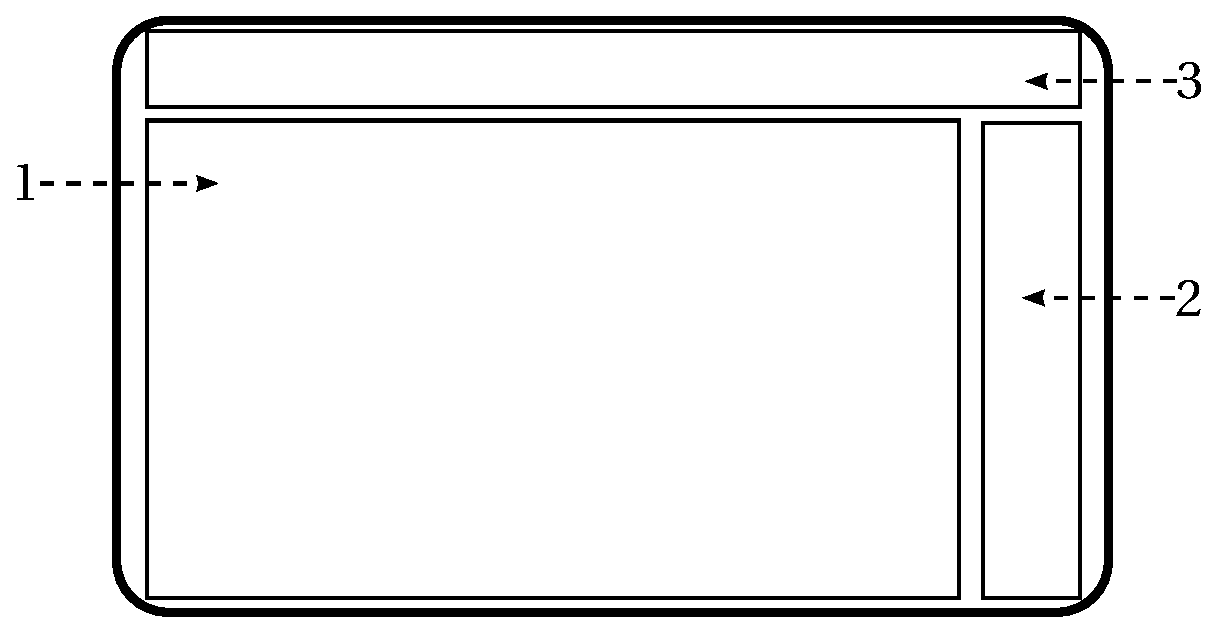
\includegraphics[width=11cm]{./Analyse/Img/14-Editeur_de_niveau.eps}
		\end{center} 
			
	\subsubsection*{Controleur}
		
		Pour finir le contrôleur aura pour but de faire la liaison entre les 
		données du modèle et de la vue.
		Chaque vue possède son controleur.
		Il y a un controleur gobal possédant les controleurs de chaque vue.
			

	\subsection{jeu}
	
	Comme vue dans le cahier des charges, l'application est divisée en 
	trois grandes parties: le modèle, la vue et le contrôlleur.
	
	\begin{center}
		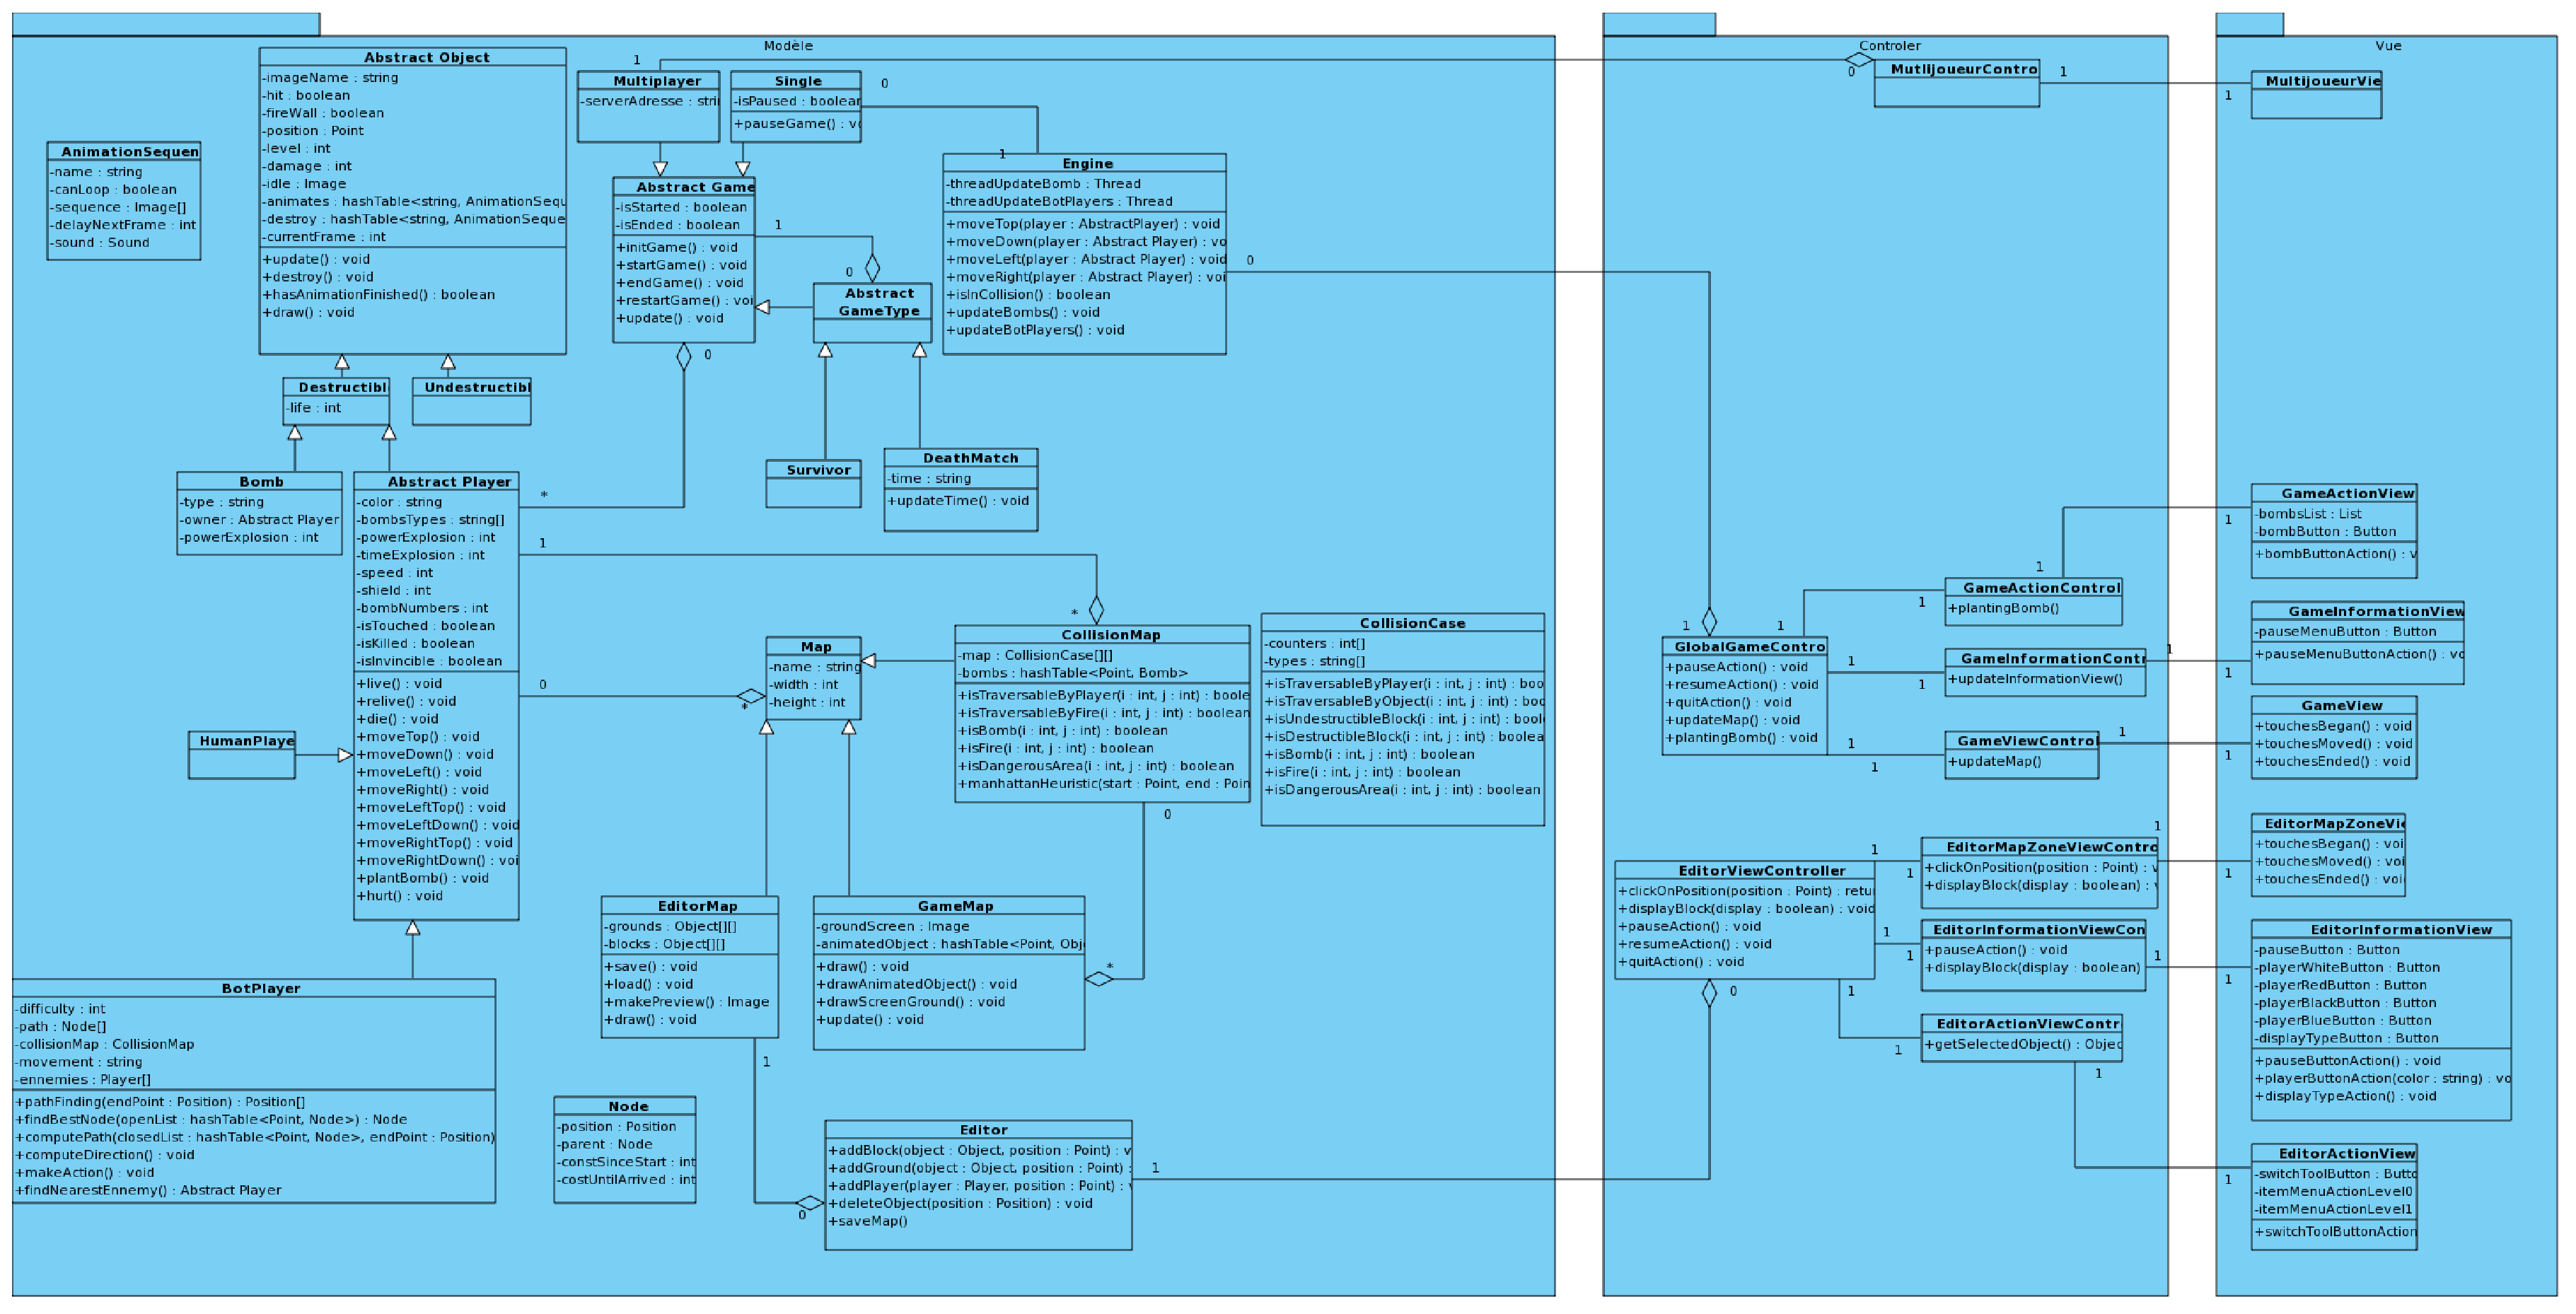
\includegraphics[scale=0.41, angle=90]{./Analyse/Img/BomberblocDiagramme.eps}
	\end{center}
	
	\subsubsection{Modèle}
	
		Le modèle constitue la \textit{base} de notre projet.
		C'est sur celui-ci que nous avons construit le reste de l'application.
		Ce dernier se décompose en trois sous-partie: la partie hierarchie des objets, la partie moteur puis la partie éditeur de carte.\\
		
	\paragraph{Hierarchie des objets \\}
	
		Pour concevoir la hierarchie des objets, il a fallu tout d'abord 
		dinstinguer la totalité des objets qui seraient disponibles dans 
		le jeu ainsi que leurs différences et leur point communs.
		
		Pour cela nous avons donc distingué quatre grands types d'objets:
		\begin{itemize}
		  \item Les destructibles
		  \item Les indestructibles
		  \item Les animés
		  \item Les inanimés
		\end{itemize}
		
		En sachant que les objets pouvaient être destructibles-animés, 
		destructible-inanimés, indestructible-animés ou indestructible-inanimés.
		Nous avons choisi que tout objet serait considéré comme un objet animé 
		pour éviter des soucis de modélisation.
		Ainsi les objets possèderont tous une sequence d'animation d'images qui
		 sera dessinée à l'écran.
		Cette dernière sera tournera en boucle dans le cas d'une animation 
		qui se répété et qui comporte plusieurs images, sinon si elle possède 
		simplement qu'une seule image.
		Nous avons ensuite dinstingué une multitude de point communs entre 
		les différents objets dont voici le nom des attributs et leur utilité : 
	
	\begin{description}
		\item [\textit{position}]{indique la position en pixel de l'objet sur l'écran}
		\item [\textit{nom}]{indique le nom de l'objet}
		\item [\textit{hit}]{est à 1 si l'objet ne peut être traversé par un joueur}
		\item [\textit{level}]{est à 0 si l'objet est sur le sol, 1 sinon}
		\item [\textit{fireWall}]{est à 1 si l'objet ne laisse pas passer les flammes des explosions (0,sinon)}
		\item [\textit{damages}]{indique si l'objet peut infliger des dommages}
		\item [\textit{idle}]{est une image qui représente l'objet en son état dit de repos}
		\item [\textit{animates}]{est une table de hachage contenant l'ensemble des images composant la sequence d'animation de l'objet (vide si inanimés)}
		\item [\textit{destroy}]{est une table de hachage contenant l'ensemble des images composant la sequence d'animation de destruction de l'objet (vide si indestructible)}
		\item [\textit{currentFrame}]{permet de connaitre le numéro de l'image courante de la sequence d'animation en cours d'affichage}
	\end{description}

		Nous avons donc décidé de concevoir une classe "Objects" pour modéliser
		 toutes ces propriétés que les objets ont en commun.
		 
		Cette classe sera abstraite car tout objet est destructible ou 
		indestructible et cela sera décris dans des classes plus spécialisés.
	
	 	Ensuite nous avons pensé à créer deux autres classes: "Destructible" 
	 	et "Undestructible" pour les objets destructible et indestructible.
	 	Ces deux classes héritent de "Objects" car elles sont des objets.
	 	
	 	Ce qui différencie ces deux classes est le champ \textit{life} qui 
	 	permet de savoir combien de fois l'objet doit etre touché par une 
	 	bombe avant d'être detruit.
	
		Nous avons ensuite dinstingué deux autres types d"objets encore plus spécifiques :
		Les joueurs et les bombes.
		Ces derniers sont des objets destructibles puisqu'ils ne durent pas 
		toute la partie selon le mode de jeu.
	
		Les bombes possèdent deux nouveaux attributs qui les différentient 
		des autres objets :
		
			\begin{description}
				\item [\textit{type}]{permet de connaitre le type de bombe}
				\item [\textit{owner}]{Joueur qui ayant posé la bombe}
			\end{description}
			
		Quant à la classe joueur celle-ci possède encore d'autres attributs :
		
		\begin{description}
			\item [\textit{color}]{Affiche à l'écran le joueur avec sa bonne couleur}
			\item [\textit{bombsTypes}]{Type de bombe qu'il peut poser}
			\item [\textit{powerExplosion}]{Porté d'explosion de ses bombes}
			\item [\textit{timeExplosion}]{Temps d'explosion de ses bombes}
			\item [\textit{speed}]{Vitesse du joueur}
			\item [\textit{shield}]{Valeur du bouclier}
			\item [\textit{bombNumbers}]{Nombre maximum de bombes que le joueur peut poser}
			\item [\textit{isTouched}]{Permet de savoir si le joueur viens d'être touché}
			\item [\textit{isKilled}]{Permet de savoir si le joueur est mort}
			\item [\textit{isInvincible}]{Permet de savoir si le joueur est invincible}
		\end{description}
	
		Cette hierarchie de classe nous permettra donc de modéliser l'ensemble 
		des objets que le jeu pourra afficher.
	
	
	\paragraph{Moteur\\}
	
		Pour ce qui est du moteur.
		Celui-ci est représenté par une classe "Engine".
		Cette classe va contenir l'ensemble des méthodes qui vont permettrent 
		d'établir les collisions.
		C'est aussi cette classe qui s'occuppe de mettre à jour les bombes 
		ainsi que l'\gls{ia} du jeu.
		
		Une instance d'un moteur est associée à une partie dont le nom de classe est "Game".
		Cette classe "Game" est abstraite et représente une partie avec toutes les options qu'elle contient.
		
		C'est à dire qu'elle possède des attributs permettant de décrire le type de partie,
		un tableau avec chaque joueur de la partie, ainsi que le carte du jeu.
		La classe possède toutes les méthodes d'initialisation, de mise à jour,
		 de dessins et de fin de la partie.
		
		Enfin pour différencier les différents types de parties nous avons utilisé
		 le \gls{pattern} décorateur.
		 Ainsi il y aura deux grands types de parties: les parties solitaires 
		 et les parties multijoueurs.
		 Puis ces parties sont décorés par le type de partie: \gls{survivor} ou \gls{death_match}.
	
		Ensuite pour ce qui est des cartes, une classe abstraite nommé "Map" 
		contient le nom et la taille de la carte ainsi qu'un tableau contenant 
		la position initial de chaque joueur sur la carte.
		
		Puis une classe "GameMap" qui hérite de map permet de dessiner 
		la carte a l'écran lors du jeu.
		Elle se compose d'une image représentant le sol puis d'un tableau 
		d'objets animés qui permet de représenter l'ensemble du reste des objets.
		
		Ensuite nous utilisons un autre type de carte qui va permettre de 
		faciliter les collisions, que ce soit pour un joueur humain ou pour 
		une intelligence artificielle.
		Cette classe est appelé "CollisionMap" et contient une matrice d'objets
		"CollisionCase" ainsi qu'un tableau qui contient l'ensemble des bombes 
		posées sur la carte.
		Les "CollisionCase" sont composées de deux tableaux.
		Chaque valeur d'un des tableaux est associée à une valeur de l'autre tableau.
		Un tableau \textit{types} contient les différents types de danger ou d'objets 
		qui existent sur cette case ainsi qu'un tableau \textit{counters} permettant 
		en fonction de chaque type de compter le nombre de fois que ce danger ou objet 
		est présent sur cette case.
		Par exemple on peut très bien avoir une case qui est dans le champ d'explosion
		de quatres bombes et qui contient un bloc de type destructible.
		
		Ainsi le tableau \textit{type} contiendra deux champs, un pour le 
		type zone dangereuse et un autre pour le type bloc destructible puis 
		le tableau \textit{counters} contiendra donc dans sa case associée à 
		la case zone dangereuse une valeur égale à quatre et et une valeur de
		un pour l'autre.
		
	
	\subsubsection{Vue}
	
		L'interface graphique du jeu est décomposée en trois parties.
		Une partie qui représente le menu d'information de la partie, 
		une autre qui réprésente le menu des actions possibles du joueurs 
		et une dernière qui représente la partie en cours.
		
		Le menu d'information se situe en haut de l'écran.
		Il permet d'afficher le score des joueurs, le temps lors d'une partie 
		death match ainsi que les bonus du joueurs (le nombre de bombes qu'il 
		peut poser, la portée de l'explosion des bombes, la vitesse du joueur 
		et les bonus de vie) et de mettre le jeu en pause.
		
		Le menu d'action se situe à droite de l'écran.
		Il permet à l'utilisateur de poser les bombes grâce à un bouton 
		et aussi de changer de type de bombes grâce à une liste déroulante.
	
		Quant à la partie, elle est affichée au centre de l'écran et prend le 
		maximum de place possible pour que le jeu soit le plus visible.
		Elle permet d'afficher la carte ainsi que les joueurs et les bombes.
		Mais elle sert aussi à écouter les mouvements du doigt de l'utilisateur
		pour modifier les coordonnées du joueur dans le modèle pour pouvoir 
		ensuite rafraichir l'écran et voir le joueur se deplacer.	
	
	
	\subsubsection{Controlleur}
	
		Le controlleur va permettre de faire la liaison entre la vue et le modèle.
		La majorité de ces méthodes sont appelées lorsque l'utilisateur interagit avec la vue.
		Ces méthodes vont par la suite modifier le modèle qui va permettre de mettre à jour la vue.
		Le controlleur est divisé en quatre sous-controlleurs.
		Chacun des trois premiers est respectivement associé à l'une des trois vues cité ci-dessus.
		Puis le quatrième est plus général, il permet de faire la liaison entre les trois autres controlleurs.
		Car en effet chacune des actions effectuées sur l'une des vues peut modifier l'une des deux autres.
	
	\subsubsection{GamePlay}
	
		Nous avons choisi d'établir un gameplay immersif.
		Notre gameplay est divisé en trois parties: les déplacements, la pose des bombes et la gestion des différents types de bombes.
		
		Pour ce qui est des déplacements du joueurs, nous avons décidé que 
		l'utilisateur utiliserait toute la surface de l'écran pour se déplacer.
		Ainsi si il veut se déplacer vers la droite, il fait glisser sont doigt 
		de la gauche vers la droite, puis tant qu'il restera appuyé sur l'écran,
		le joueur continura de se déplacer.
		Cette manière de se déplacer est précise et très intuitive contrairement
		à l'utilisation d'un joystick virtuel ou de l'accéléromètre.
		
		Pour la pause des bombes un simple boutton est mit en évidence en bas à
		 droite de l'écran.
		 Celui-ci est assez gros pour que l'utilisateur n'est pas à appuyer sur
		 une zone trop précise en cas de manipulation rapide.
		
		Puis pour le choix des différentes bombes, une simple liste déroulante 
		est mise en évidence à droite du jeu.\\
		
		\subsubsection{Tile Mapping}

			La gestion des images a été une partie très importante de l'analyse
			car le développement mobile impose plusieurs contraintes, notamment 
			la gestion de la mémoire et la vitesse d'affichage.
			
			Nous nous sommes donc inspirés des premiers jeux consoles comme 
			Super Mario Bros ou Zelda qui ont été développés sur les premières 
			consoles comme la \gls{nes} ou la \gls{game_boy}.
			Nous avons donc conçu le moteur du jeu selon le principe du \gls{tile_mapping} 
			pour minimiser l'utilisation des ressources des téléphones.
		
			Le principe du Tile Mapping est d'utiliser des petites images que nous appelerons \textit{tiles}.
			Ces tiles sont toutes contenues dans une image.
			Ensuite une matrice de nombre entier est utilisé pour représenter l'environnement du jeu.
			Chaque nombre entier représente un tile.
			Puis grâce à cette association, la carte sera dessiné à l'écran selon la matrice.
			Voici un exemple :
		
			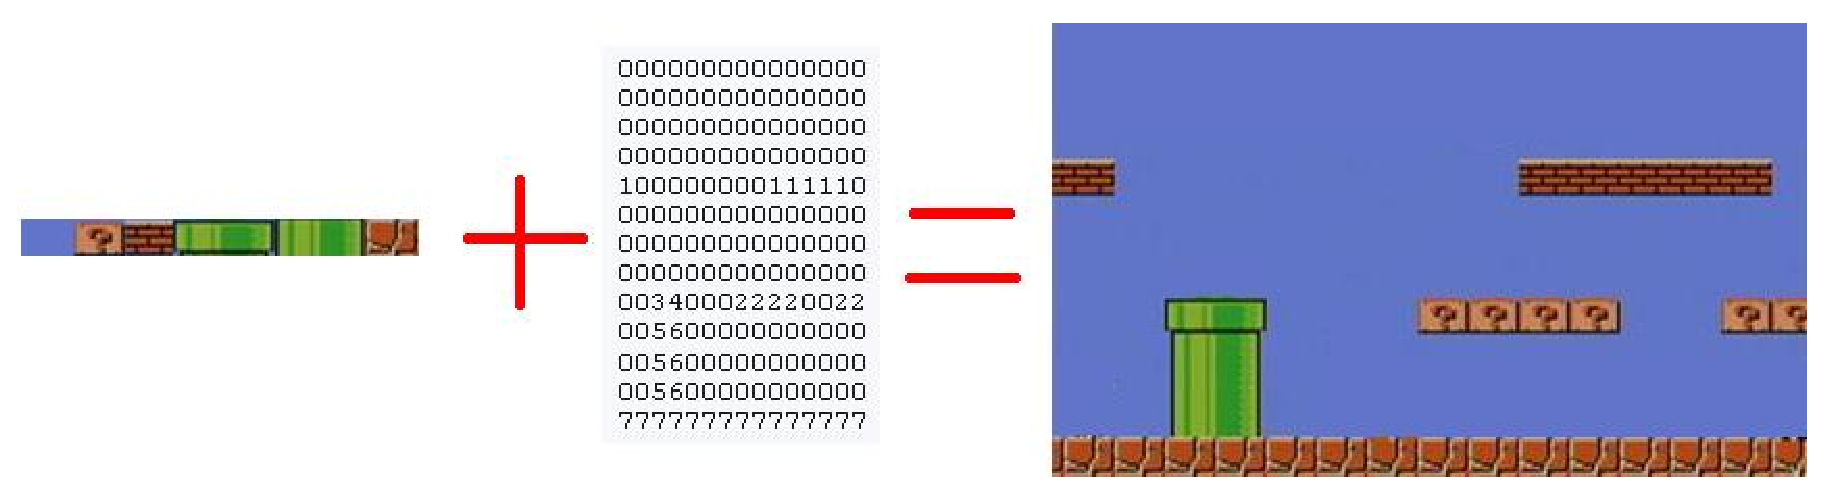
\includegraphics[width=15cm]{./Analyse/Img/tileMapping.eps}
		
			Pour pouvoir animer certains de ces objets nous avons utilisé des sprites.
			Les sprites contrairement aux tile sont un ensemble d'images représentant
			une animation.
		
			Nous avons donc repris ce principe et nous l'avons amélioré.
			En effet grâce à la programmation objet, les entiers sont réprésenté directement par des objets
			contenant les tiles/sprites qui les représentent.
			
			Ainsi, nous stockons dans une matrice tous les objets inanimés
			(les objets dont le tile restera le meme tout le long de la partie)
			et nous parcourons cette matrice pour dessiner chaque objet à sa 
			position pour obtenir une nouvelle image au format png.
			A chaque rafraichissement de l'écran, seule la nouvelle image est dessinée 
			et non pas chaque tile.
			Cette méthode permet d'éviter un parcours intempestif de la matrice.
			
			Ensuite pour le reste des objets dit animés (repésentés par des sprites)
			nous avons décidé de les stocker dans une table de hachage dont la 
			clé est la position de l'objet (pour y accéder plus rapidement).
			Lors du rafraichissement de l'écran on parcourra entierement la 
			table de hachage et l'on dessinera l'image courante de la sequence 
			d'animation de chaque objet.
		
		\subsubsection{La gestion des images et du son}
		
			Chaque image et chaque son dont est composé le jeu sont chargés au lancement de l'application.
 			
 			Afin de pouvoir ajouter facilement un objet et le modifier sans avoir à toucher au code
 			source, nous avons décidé d'opter pour les stocker sur des fichiers au format \gls{xml}
 			Les fichiers \gls{xml} ressemblent tous plus au moins a ce genre d'arborescence: 
		
		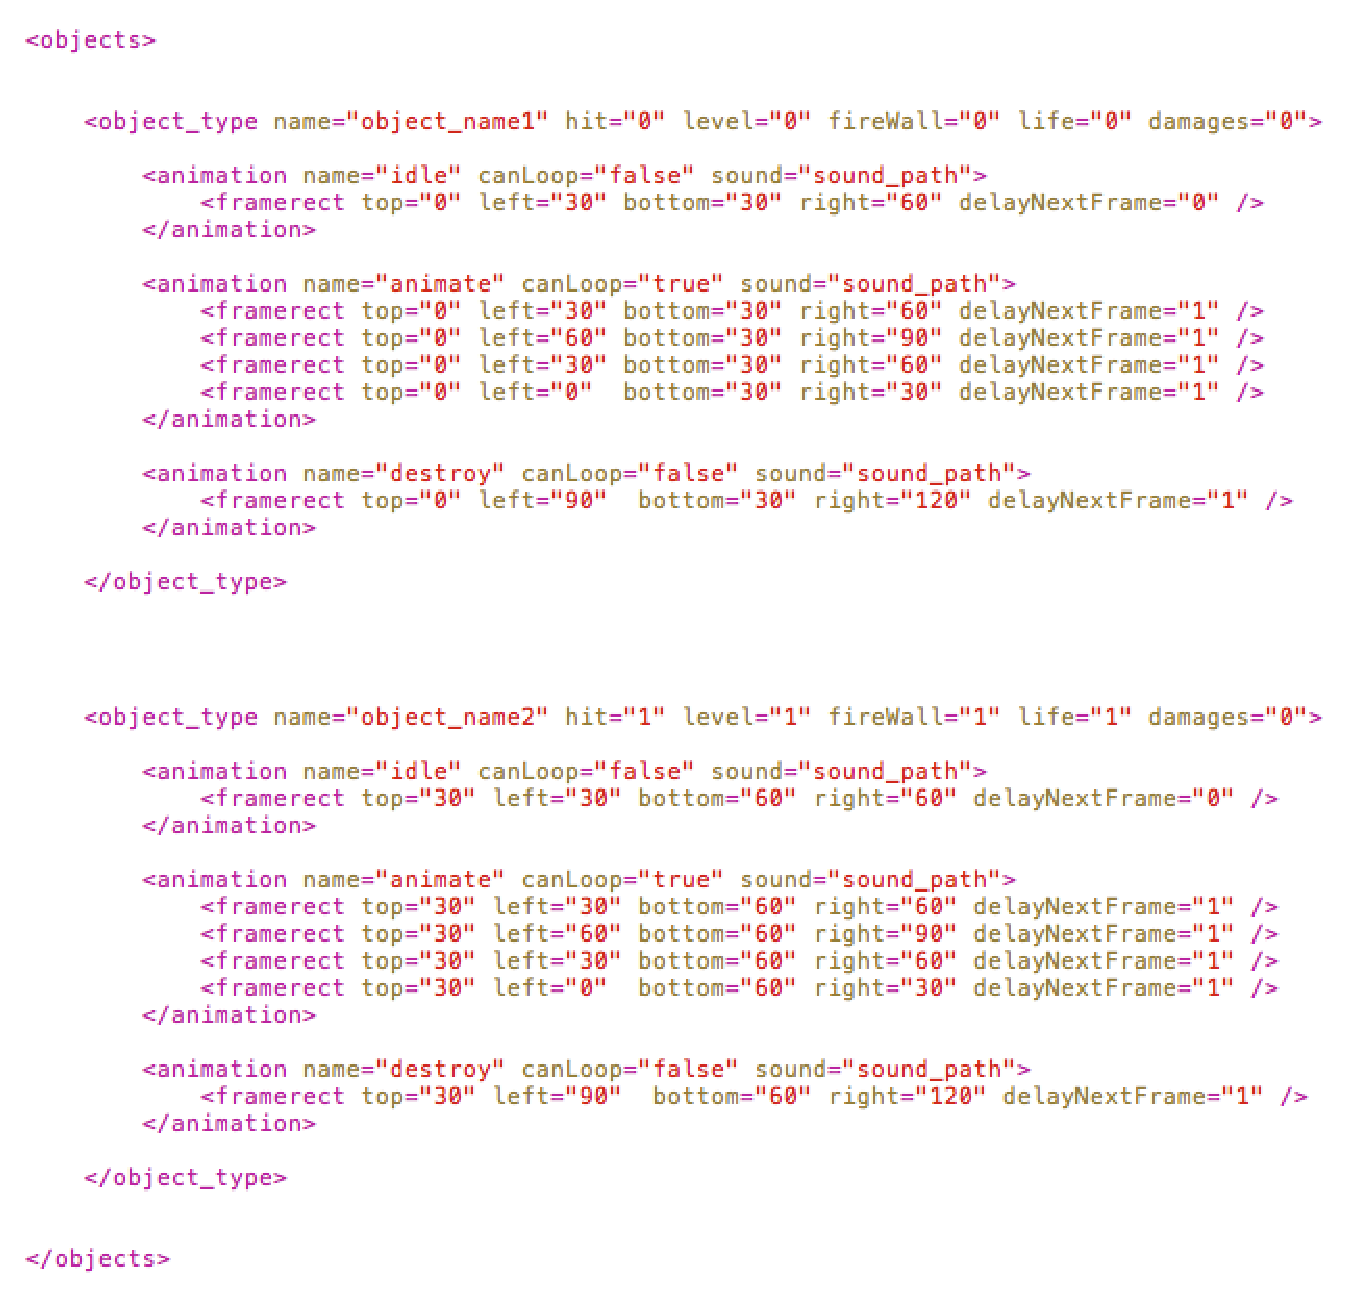
\includegraphics[width=15cm]{./Analyse/Img/exampleXmlBomberklob.eps}
		
			Chaque fichier \gls{xml} commence par une balise racine permettant 
			de lister les objets qu'elle contient (\textit{<objects>}).
			Ensuite chaque objet est décris par une balise  qui contient le type,
			le nom de l'objet ainsi que l'ensemble de ses propriétés.
			
			La propriété \textit{hit} est à 1 si l'objet n'est pas traversable par un joueur (0, sinon), 
			le champ \textit{level} est à 1 si l'objet se trouve au premier niveau de la carte (0,sinon), 
			le champ \textit{fireWall} est à 1 si l'objet ne laisse pas passer les flammes des explosions, 
			le champ \textit{life} indique le nombre de fois que l'objet doit etre touché
			et enfin le champ \textit{damages} indique si l'objet peut infliger des domages.
			
			Par exemple \textit{<destructible name="herb" hit="1" level="1" fireWall="1" life="1" damages="0">} 
			décris un objet de type \textit{destructible}, qui n'est pas traversable, se trouvant au niveau
			1 sur la carte, ne laissant pas passer les flammes des bombes, possedant une vie, 
			n'infligeant pas de dommage et dont le nom est \textit{herb}.
			
			Ensuite chaque objet possède au plus trois balises animations (sauf pour les joueurs).
			Tout objet possède au moins la premiere balise: 
			<animation name="idle" canLoop="false" sound="sound\_path"> 
			qui est celle dont le nom est \textit{idle}.
			
			Elle représente l'image standard de l'objet.
			Par exemple pour un objet bombe, ce sera l'image qui sera affichée dans la liste des bombes 
			pour pouvoir selectionner ses bombes.
			Le champs \textit{canLoop} permet de savoir si l'animation doit être répétée en boucle 
			et le champ \textit{sound} contient le chemin d'accès au fichier de son de l'animation 
			si elle en possede un.
			
			Il y a ensuite la balise mais dont le nom est \textit{animate}, celle-ci contiendra *
			toutes les sequences d'images d'un objet qui est animés.
			La dernière est celle dont le nom est \textit{destroy} et qui contiendra 
			l'ensemble des images composant la sequences d'animation de destruction de l'objet.
			Enfin chaque balise de type animation contient des balises de type \textit{framerect}.
			Ces balises permettent de donner la position de chaque image de la séquence d'animation
			dans la bitmap globale ainsi que le delai de rafraichissement entre chaque image.
			Par exemple \textit{<framerect top="60" left="30" bottom="90" right="60" delayNextFrame="1" />}
			représente une image dont le bord du haut est situé à 30pixels, le bord du bas à 90pixels, 
			le bord de gauche à 30pixels et le bord de droite à 60pixels en partant du coin en haut à 
			gauche de l'image globale.
			Puis pour le champ \textit{delayNextFrame} celui-ci informe que l'image suivante sera déclenchée 
			apres un delay de 1s.\\
		
			Grâce à cette modélisation, l'application va parcourir au démarrage l'ensemble des fichiers 
			XML et va créer une table de hachage pour chaque ensemble d'objet du fichier.
			Lors de ce parcours, l'application va instancier chaque objet avec toutes propriétés 
			que lui indique le document XML, ainsi que ses sequences d'animations.
			Ensuite lorsqu'un objet devra être utilisé dans le jeu, il suffira d'utiliser 
			une copie de l'objet déja chargé en mémoire pour éviter d'avoir à reparcourir le fichier.
			
			
	\subsubsection{Intelligence artificielle}
	
		Comme nous avons vu dans le cahier des charges, nous avons mis en 
		place une intelligence artificielle permettant à un joueur de jouer 
		en solotaire.
	
		Tout d'abord nous avons dû réfléchir à toutes les actions que les 
		\glspl{bot} pourraient effectuer, lors d'une partie.
		
		L'intelligence artificielle dans notre jeu utilise des algorithmes de \gls{recherche_op}.
		
		Pour une meilleure expérience de jeu nous avons séparé l'intelligence artificielle en trois niveaux.
		
		$\,$
		
		\begin{itemize}
		  \item Facile
		  \item Moyenne
		  \item Difficile
		\end{itemize}
		
		$\,$
		
		Nous avons utilisé deux types d'algorithmes de \gls{recherche_op} basés sur le \gls{pathfinding}.
		
		\paragraph{Pathfinding}
		
			Le premier algorithme basé sur le parcours en largeur est utilisé quel que soit
			le niveau de l'intelligence artificelle choisie contrairement au second qui n'est utilisé
			que pour la difficulté moyenne et difficile.
		
		\subparagraph{Parcours en largeur\\}
		
			L'algorithme du parcours en largeur dans notre cas, consiste à partir d'un sommet S,
			lister d'abord tous les voisins de S pour ensuite les explorer un par un.
			Ici nous allons donc regarder toutes les cases autour de nous puis regarder
			tous leurs voisins et cela ainsi de suite jusqu'à trouver un point
			correspondant à nos attentes.
			
			Le contexte est le suivant, un \gls{bot} découvre qu'il est sur la trajectoire
			d'explosion d'une bombe est va donc fuir vers la case sûr la plus proche or
			il n'a aucune idée d'où elle se trouve.
			
			L'image suivante représentera la situation initiale :
			
			\begin{center}
				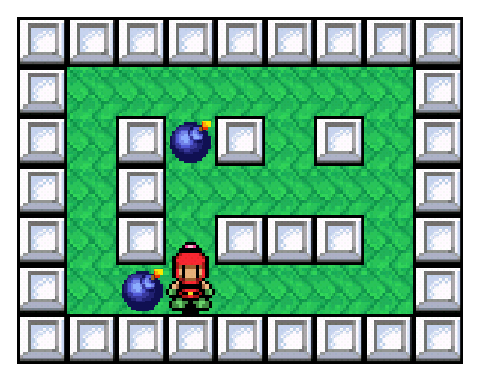
\includegraphics[width=8cm]{./Analyse/Img/largeur_0.eps}
			\end{center}
			
			Comme dit précédemment il n'y a que les murs ou les bombes que l'on ne peut
			pas traverser sinon tous les autres objets ou joueurs sont traversables.
			Nous considerons que les bombes ont ici un champs d'explosion en nombre de
			cases de 5.			
			
			Représentons la carte ci-dessus d'une façon plus parlante en remplacant les
			divers objets mis à par le joueur par des couleurs leur correspondant, à
			savoir :
			
			\begin{center}
				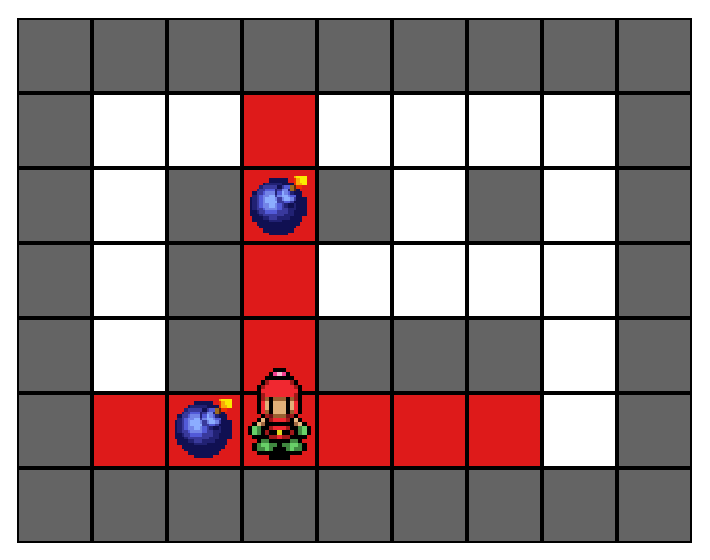
\includegraphics[width=8cm]{./Analyse/Img/largeur_1.eps}
			\end{center}
			
			Mettons nous à present à la place du \gls{bot}.
			
			Nous allons donner un poid aux cases que nous allons parcourir
			correspondant à la distance par rapport à la case initiale, ainsi qu'une
			direction qui correspondra à la direction initiale que le \gls{bot} devra empruter
			pour utiliser ce chemin, c'est à dire par exemple que tout chemin découvert
			dont l'origine est une case à droite de la notre aura comme direction droite.
			
			A partir d'une case donnée, nous ne regarderons que les voisines ayant un poids de 0
			car si leur poids est différent cela voudra dire que nous les avons déjà vu precedemment et bien évidemment,
			nous ignorerons les murs ainsi que les bombes.
			
			Nous avons changé la valeur des cases intraversables pour ne pas confondre avec le poids des cases visitées.			
			
			Appliquons l'algorithme de parcours en largeur aux cases voisines de la notre.
			
			
			\begin{center}
				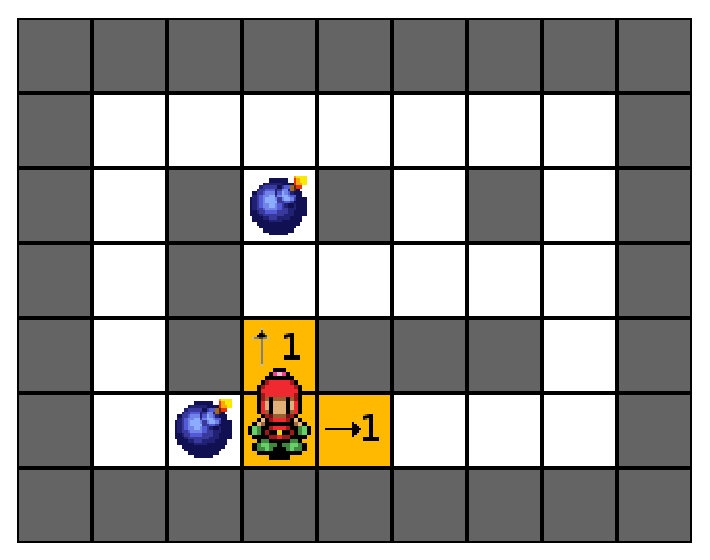
\includegraphics[width=8cm]{./Analyse/Img/largeur_2.eps}
			\end{center}
			
			
			Toutes les cases découvertes étant considérées comme dangereuses (voir le schéma précédent) nous continuons à appliquer l'\gls{algorithme} jusqu'à arriver à notre but.
			
			\begin{center}
				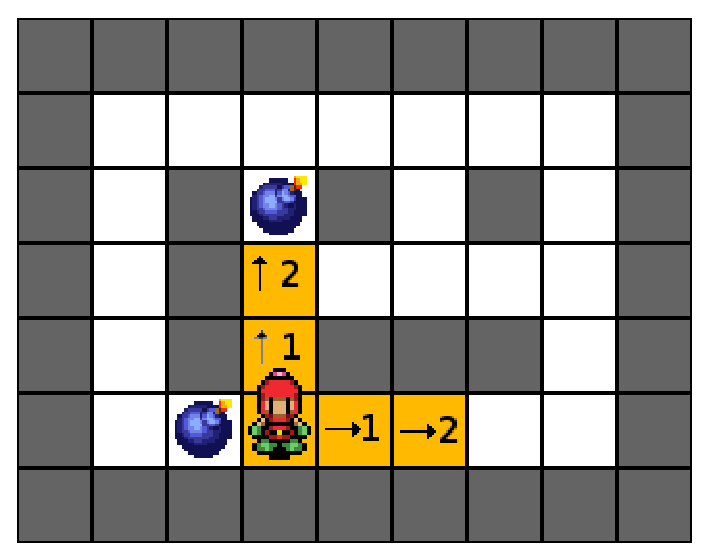
\includegraphics[width=8cm]{./Analyse/Img/largeur_3.eps}
				
				$\,$
				
				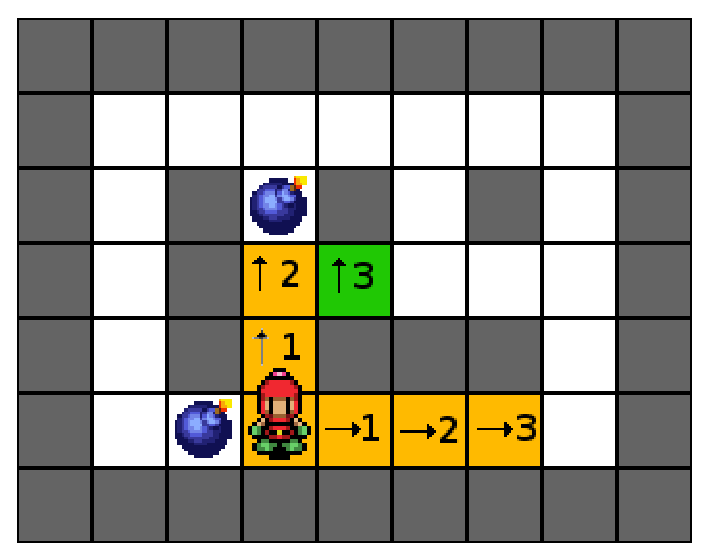
\includegraphics[width=8cm]{./Analyse/Img/largeur_4.eps}
			\end{center}
			
			Ici nous avons découvert une case non dangeureuse en $(13,6)$.
			
			Nous récupérons donc la direction enregistrée dans cette case et bougeons en fonction de celle-ci.
			
			Si plusieurs cases avaient été découvertes le choix aurait été arbitraire car elles auraient toutes été à la même distance.
			
			$\,$
			
		\subparagraph{A*\\}
		
			L'action la plus importante que l'intelligence artificielle doit savoir faire c'est de pouvoir se déplacer librement sur la carte en fonction des différents objets présents sur la carte et des actions effectuées par les autres joueurs.
		
			L'algorithme de recherche A* a pour but de rechercher un chemin
			dans un graphe entre un nœud initial et un nœud final tous deux préalablement
			définis. A* permet de trouver l'un des meilleurs (mais pas forcément le
			meilleur) chemins existant entre un point A et un point B (il retourne le premier chemin trouvé).
			
			La force de cet algorithme est le temps de calcul et l'exactitude des résultats, contrairement à Dijkstra qui lui fournit toujours le meilleur résultat (le plus court chemin entre deux points) mais dans un temps d'exécution beaucoup plus long que l'algorithme de A*.
			
			Sachant qu'il peut y avoir jusqu'à trois \glspl{bot} et que l'intelligence artificielle doit régulièrement recalculer son chemin en fonction des actions effectuées par les autres joueurs, nous avons donc choisi l'algorithme de A*.
		
			Maintenant que l'on sait quel algorithme utiliser pour rechercher un chemin dans un graphe, nous allons voir en détail comment marche l'algorithme de A*.
		
			Pour comprendre comment l'algorithme marche, nous allons nous aider d'un
			dessin représentent une carte avec un point A (départ) affiché en vert, un
			point B (arrivée) en rouge, et où les cases en bleu représentent les murs.
		
			\begin{center}
				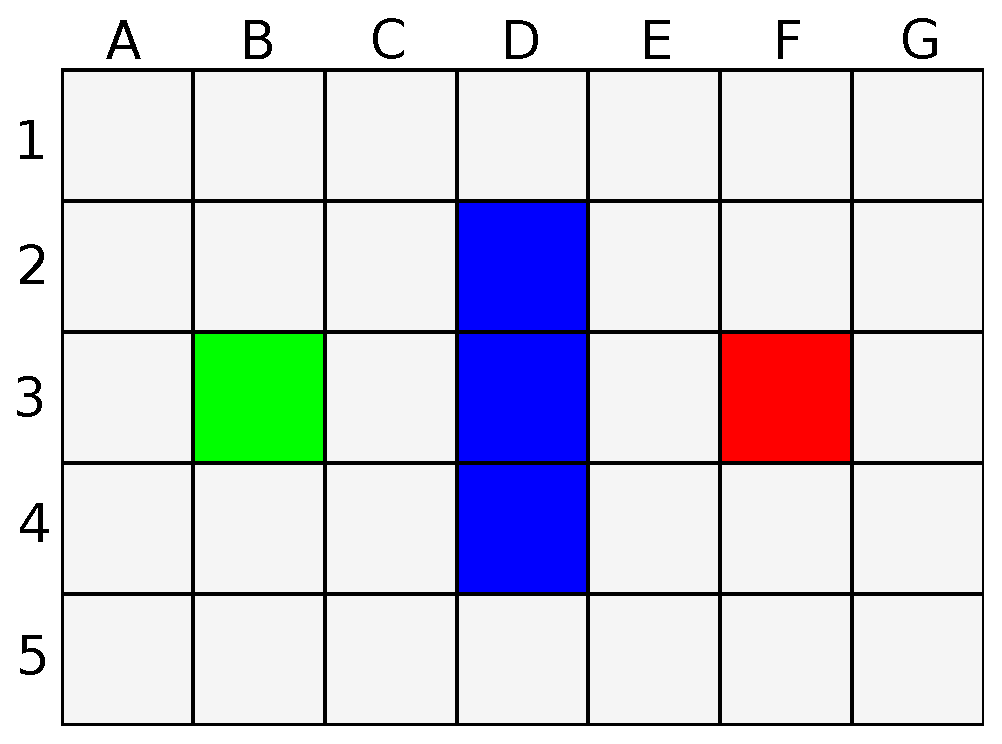
\includegraphics[width=8cm]{./Analyse/Img/Grille.eps}
			\end{center}
		
			La premier chose que l'on peut observer, c'est que la carte est divisée en
			cases. Chaque case de la matrice représente un node qui peut être soit
			traversable, soit non traversable. Dans l'application, il n'y a que les murs
			ou les bombes que l'on ne peut pas traverser sinon tous les autres objets
			ou joueurs sont traversables. Le but de l'algorithme est donc de
			trouver un chemin entre A et B en évitant les murs.
			
		
			Durant le déroulement de l'algorithme, nous avons utilisé deux listes qui contiennent des cases de la carte.
			Il y a une liste dite \og listeOuverte \fg \, et l'autre \og listeFermée \fg.
			La listeOuvrete contient une liste de cases qui pourraient éventuellement faire partie du chemin, mais pas forcément, pour le moment elle sera vide.
			Plus précisément c'est une liste de cases que nous devons vérifier.
			Ensuite, au niveau de la listeFermée, elle contient toutes les cases que nous
			aurons déjà vérifiées, au début de l'excution, elle contient que le point de départ (B3).
			
		
			Commencons les explications du déroulement de l'algorithme.
			Tout d'abord, il faut savoir qu'un joueur peut se déplacer dans toutes les
			directions, donc nous allons ajouter toutes les cases adjacentes à la
			listeOuvert qui sont traversables, il y en a huit (A2, B2, C2, A3, C3, A4, B4, C4).
			
			
			Ce qui nous donne :
		
			\begin{center}
				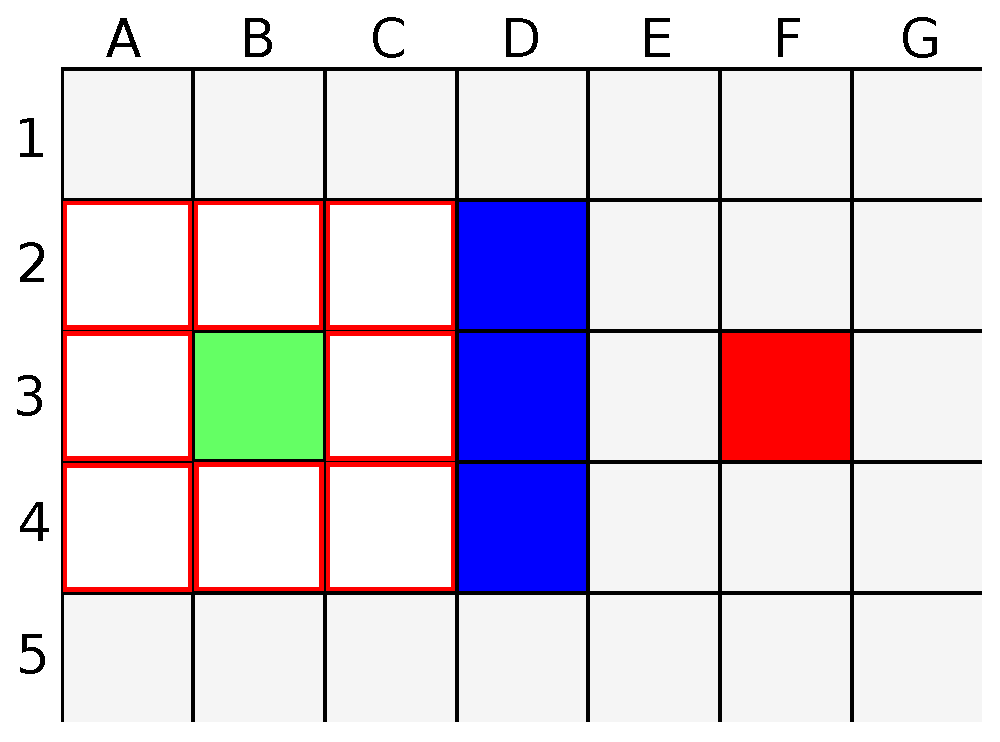
\includegraphics[width=8cm]{./Analyse/Img/Grille2.eps}
			\end{center}
		
			Les carrés avec un contour rouge sont les carrés présents dans la
			listeOuverte et les carrés qui ont une couleur un peu plus foncée que les
			autres sont ceux qui se trouvent dans la listeFermée.
		
			Maintenant pour choisir la case par laquelle on doit passer, nous devons rajouter trois données \og F \fg , \og G \fg \, et \og H \fg:
			\begin{description}
				\item[G : ]{c'est le coût de mouvement pour aller de la case A à une case donnée sur la grille, en suivant le chemin généré jusqu'à cette dernière.}
				\item[H :]{c'est l'heuristique, c'est à dire le coût estimé pour allé du point courant à l'arrivé. Comme nous ne connaissons pas vraiment la distance qu'il nous reste à parcourir, car toutes sortes d'obstacle peuvent se trouver sur notre chemin (objet non traversable). Donc nous allons devoir l'approximer grâce à une fonction, pour la calculer nous avons choisi d'utiliser l'heuristique de Manhattan, qui consiste à compter le nombre de bloc (à vol d'oiseau et sans prendre les diagonales) qui lui reste à parcourir.}
				\item[F :]{c'est G + H}
			\end{description} 
		
			Chaque case de la listeOuverte ou de la listeFermée vont devoir possèder toutes ces données, plus les coordonnées de leur père, c'est à dire les coordonnées de la case qui vient de les ajouter dans la la listeOuverte. Pour calculer G, nous allons assigner un coût de 10 pour chaque déplacement horizontal ou vertical, et un coût de 14 pour un mouvement en diagonale. Nous utilisons ces données car la distance nécessaire pour se déplacer est la racine carrée de 2, ou approximativement 1.41 fois le coût d'un déplacement vertical ou horizontal. Nous utiliserons donc 10 et 14 pour des raisons de simplification. Par conséquent, nous allons multiplier par 10 le coût H pour qu'il soit cohérent par rapport à G.
	
			Donc maintenant, nous devons avoir cette matrice :
			\begin{center}
				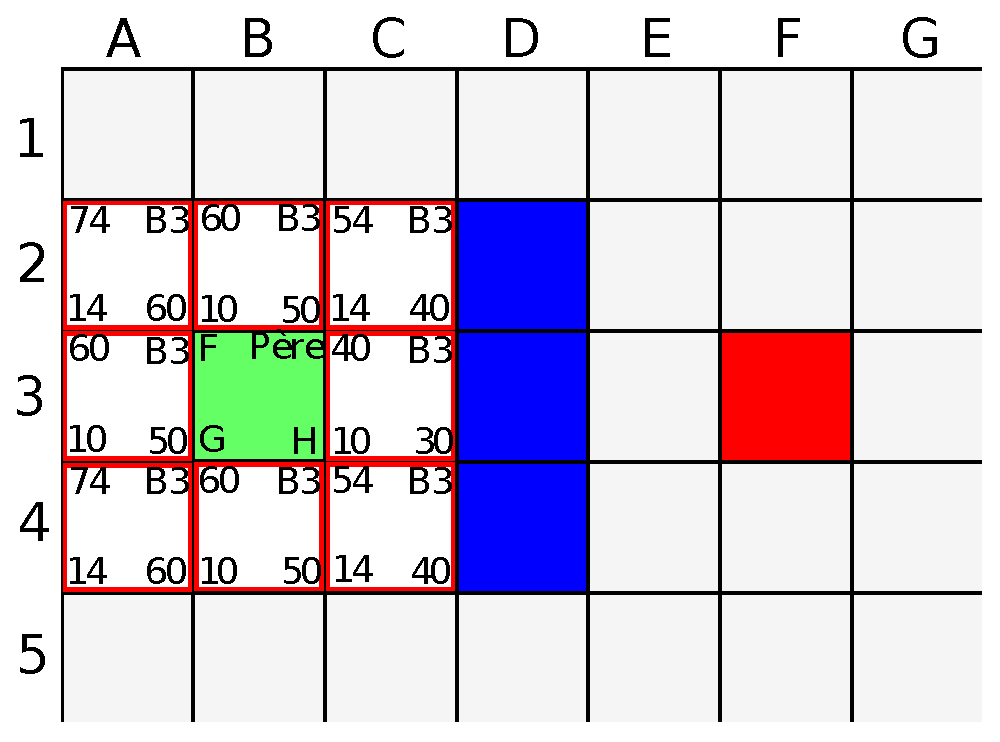
\includegraphics[width=8cm]{./Analyse/Img/Grille3.eps}
			\end{center}
		
			Après avoir ajouté toutes les cases adjacentes à la case courant, il suffit de prendre la case qui a le plus petit coût F et ensuite de la rajouter dans la listeFermée et de la supprimer de la listeOuverte. Nous obtenons donc :
			\begin{center}
				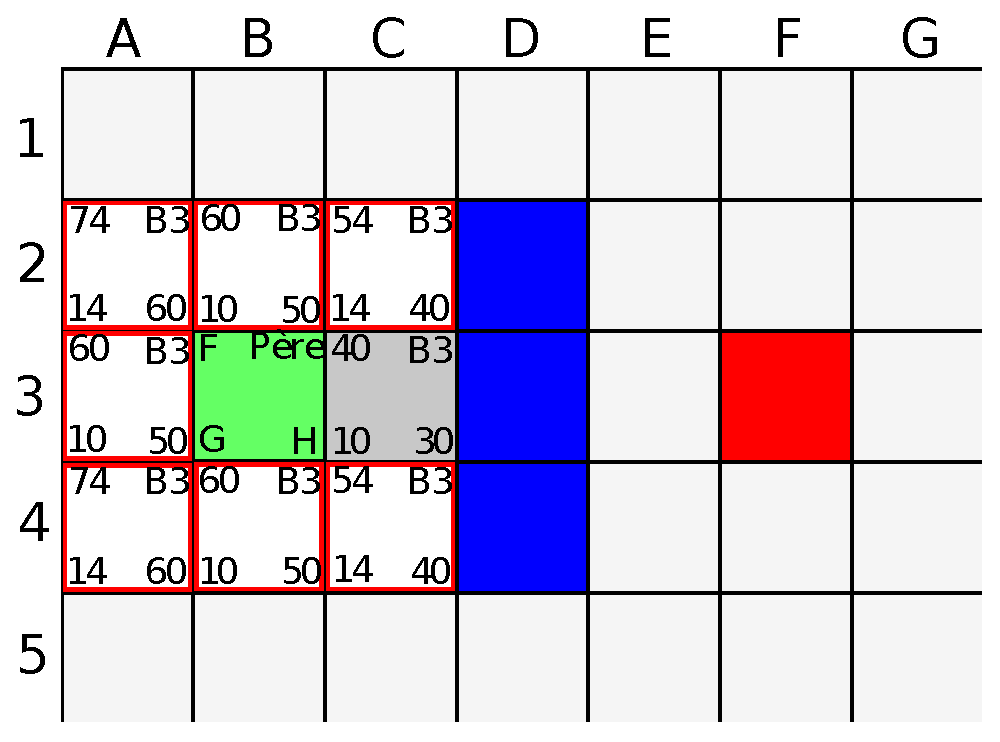
\includegraphics[width=8cm]{./Analyse/Img/Grille4.eps}
			\end{center}
		
			Ensuite on regarde toutes les cases adjacentes à la dernière case ajoutée dans la listeFermée. Si elles se trouvent déjà dans la listeOuverte, on vérifit que leurs coût soient inférieur au coût de la case correspondante déjà dans la listeOuverte, si oui alors on la remplace sinon on ne fait rien.
		
			Pour finir on répète cette opération jusqu'on arrive à la case d'arrivée, nous obtenons ça :
			\begin{center}
				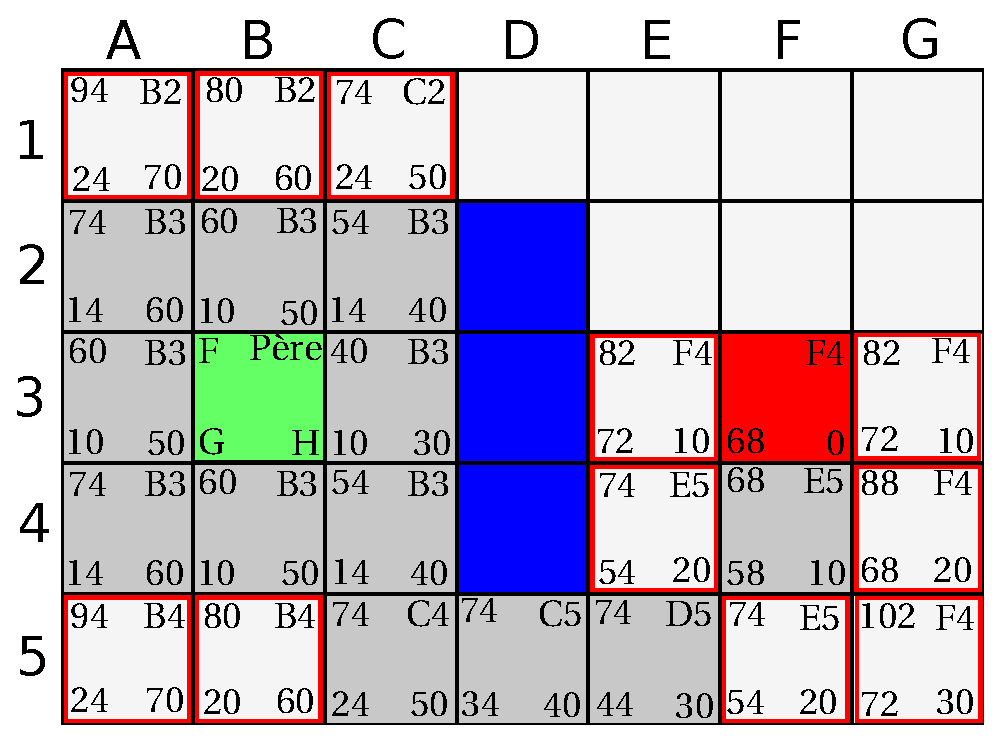
\includegraphics[width=8cm]{./Analyse/Img/Grille5.eps}
			\end{center}
		
			Pour finir, il nous suffit juste de récupérer la case d'arrivée et de regarder son père, puis de repéter cette opération avec la case obtenu jusqu'à arriver à la case de dépard. Grâce à ça nous obtenons cette dernière étape de l'algorithme :
			\begin{center}
				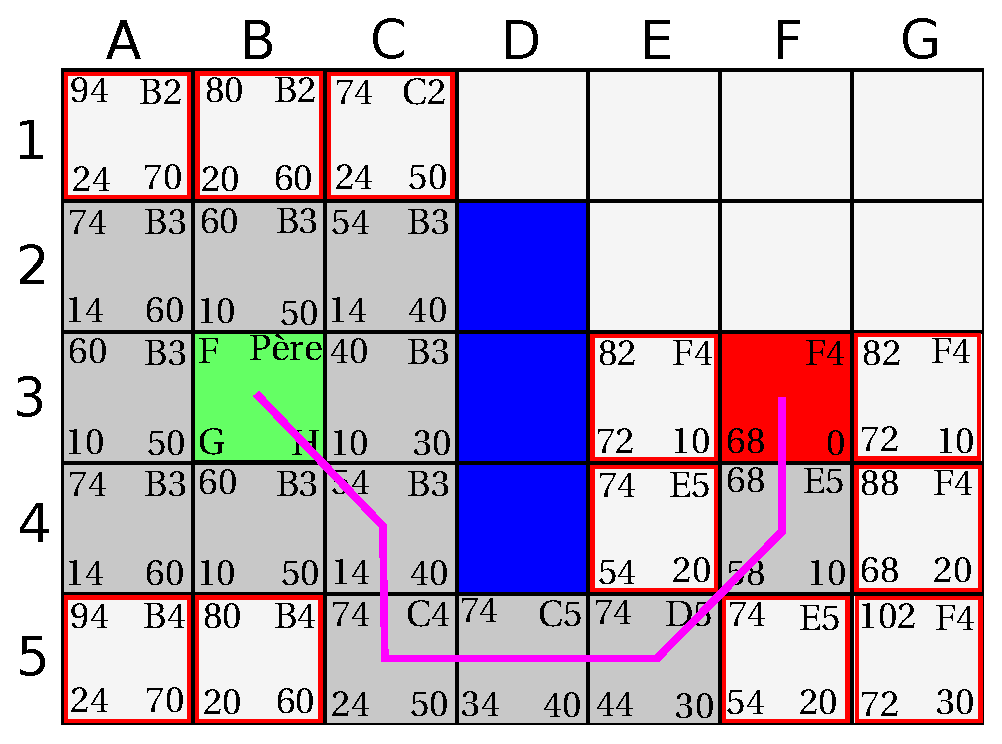
\includegraphics[width=8cm]{./Analyse/Img/Grille6.eps}
			\end{center}
		
			Comme nous pouvons levoir sur le schéma precedent, le chemin qu'a trouvé l'algorithme de A* est le suivant : $ B3 \rightarrow C4 \rightarrow C5 \rightarrow D5 \rightarrow E5 \rightarrow F4 \rightarrow F3 $. L'algorithme aurait pu d'autre chemin équivalent à celui-ci mais le principe de cette algorithme c'est de renvoyer le permier chemin qu'il trouve.


\subsection{Réseau}
		
	\paragraph{Serveur\\}
			
		Il a été fixé dans le cahier des charges que notre serveur devrait pouvoir
		effectuer plusieurs tâches particulières séparées. Nous avons donc décidé de
		les compartimenter en classes.
		
		Notre serveur est crée sur une base de servlet. Ce fût ici
		aussi un point nouveau pour nous, réiterant les phases d'analyse, de
		découverte, de test et de mise en place. Le fonctionnement est basé sur les
		échanges de requêtes type HTTP, où à chaque demande correspond une réponse. 
		
		Une servlet est une classe Java qui permet de créer dynamiquement des données
		au sein d'un serveur HTTP. Une servlet s'exécute dynamiquement sur le serveur
		web et permet l'extension des fonctions de ce dernier, typiquement : accès à
		des bases de données.
			
		Les six éléments situés sur la partie haute du schéma
		ci-dessous(respectivement ServletInscription, ServletConnection,
		ServletGamesList, ServletCreateGame, ServletConnectionGame et
		ServletManageGame), représentent les différentes tâches qu'un utilisateur
		puisse demander au serveur. Elles sont reliées à une classe nommée
		ContextListener, qui leur permettra d'accéder aux mêmes données sans qu'il y
		ait de conflit. La partie basse représente les objets qui seront utilisés 
		pour les parties en multijoueur. 
		Bien évidemment ces objets sont très proches de ceux utilisés dans les parties
		locales(Schéma 3.3).
		
		
		Comme il a été dit précédement, notre serveur est accessible via des requêtes
		HTTP contactant des servlets. Ces servlets sont stockées dans un serveur
		d'application nommé Apache Tomcat. Il s'agit d'un conteneur libre de
		servlets Java 2 Enterprise Edition, mais il fait aussi office de serveur
		Web.\\
		Un scénario probable serait qu'un utilisateur désire jouer
		en ligne contre de vrais joueurs. 
		Il passera par l'inscription et créera son compte sur le
		serveur(Inscription). Une fois cette étape obligatoire faite, il choisira
		entre rejoindre une partie en ligne en cour(ConnectionGame), ou en créer un nouvelle(CreateGame).
		Dès lors qu'il accèdera à une partie en
		ligne, un contact régulier avec le serveur sera obligatoire afin de réaliser
		les interactions entre les joueurs(ManageGame). Tout ceci se
		réalisera dans une durée infime afin de ne pas pénaliser les joueurs.	
		
		\begin{figure}
			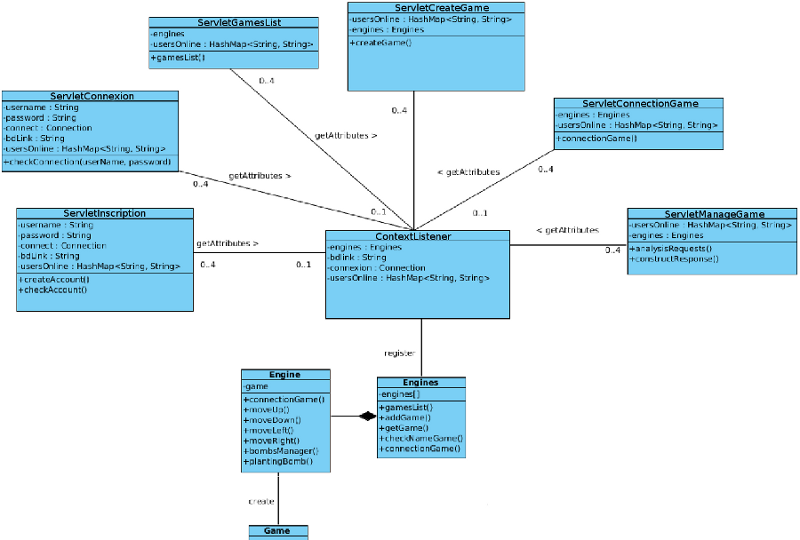
\includegraphics[scale = 0.5]{Analyse/Img/serveur.eps}
			 \caption {Serveur}
		\end{figure}
		
		\newpage
		
		
	\paragraph{JSON\\}	
	
		Soucieux des performances et de la rapidité des échanges entre applications et
		serveur, nous avons mis en place un protocole de communication client/serveur
		où les messages transitant sont des flux \gls{json}. 	
		Contrairement au \gls{xml} qui peut représenter des données orientées document,
		\gls{json} se focalise sur la description d’objets.
		Un autre avantage reconnu de \gls{json} par rapport à \gls{xml} est qu’il est nettement
		moins verbeux que ce dernier.
		Quoi qu’il en soit \gls{json} reconnait la philosophie des services web exposant
		une interface d’échange : il s’agit
		d’envoyer et de recevoir des informations dans un format facilement manipulable par
		le protocole de transport \gls{http}.
		
		
		Voilà pourquoi le \gls{json} semblait être un format de données d'échanges optimal
		pour véhiculer le plus d'informations avec une taille moindre. Il est aussi en
		adéquation avec notre politique d'utilisation web pour un serveur.
		De plus étant beaucoup utilisé, nos deux
		langages mettent à disposition des outils de sérialisation de leurs objets en \gls{json}
		
		Ci-dessous un exemple concret de notre protocole de communication \gls{json} entre
		serveur et application cliente.
		
			
		\begin{verbatim}
			ServletInscription
				Player => Serveur
				{["username","password"]}
				
				Serveur => Player
				{"OK"} ou {"BU"}
				
			ServletConnexion 	
				Player => Serveur
				{["username","password"]}
				
				Serveur => Player
				{"OK"} ou {"BU"}
				
			ServletGameList
				Player => Serveur
				{"userKey"}
			
				Serveur => Player
				{[{"class":"Game","map":"mapName","name":"gameName",
				 "playerNumberConnected":nbConnected,"type":"gameType"},{..},{..}]}
				 
			ServletCreateGame:
				Player => Server:
					{"userKey": <userKey>, 
					"game": {"name":<name>, "type":<type>, "map":<map>, "ennemiesNumber": <ennemiesNumber>}}
					
				Server => Player:
					{"OK"} ou {"errorType"}
				 
			ServletConnectionGame:
				Player => Server:
					{["userKey", "gameName"]}
					
				Server => Player:
					{[<1/2/3/4>, "play<true/false>", "map", "time<mm:ss>"]} 
					ou 
					{"errorType"}
					
			ServletManageGame:
				Player => Server: 
					{"userKey", "gameName", "action"}	
					
				Server => Players: (Player, bombs, blocs, score, time)
					{[
					 [ ["x", "y", "direction", "dead <true/false>"],[...] ],
					 [ ["x", "y", "type", "explode <true/false>" ], [...] ],
					 [ ["position": {"x", "y"}, "bonus": <bonus>], [..] ],
					 [1,2,3,4],
					 "time <mm:ss>"]} 
					 ou 
					{"errorType"}
				 
				 
		\end{verbatim}	
		
	

	\subsubsection{Schéma de fonctionnement }
		
		\begin{center}
			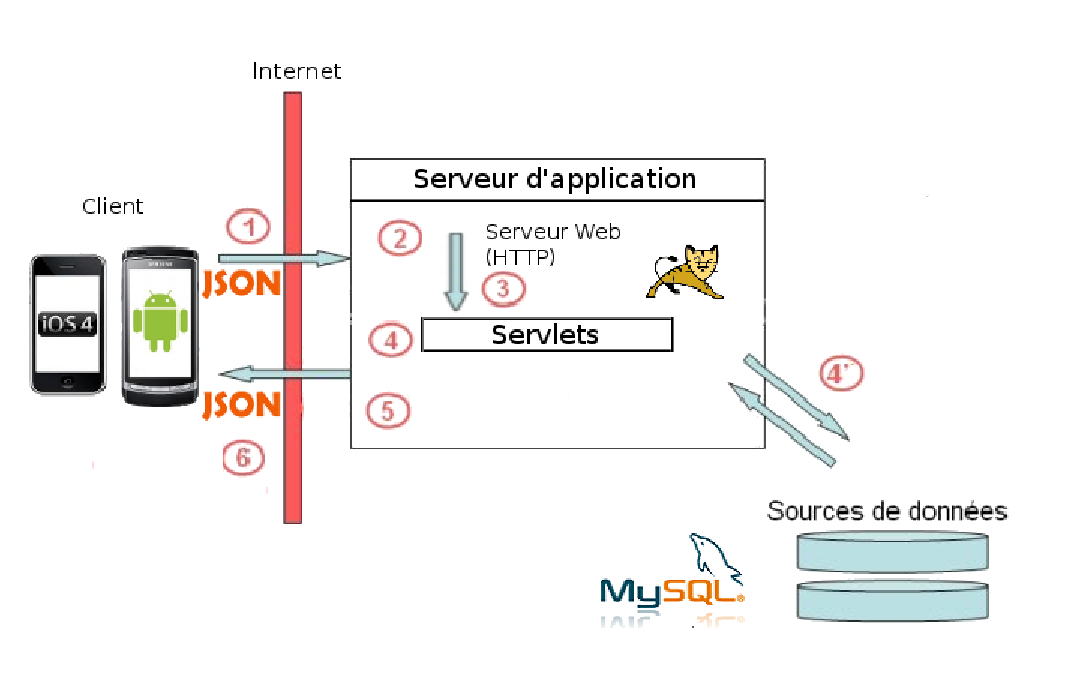
\includegraphics[width=16cm]{Analyse/Img/4.eps}
		\end{center}
		
		\begin{enumerate}

			\item 
					Le client émet une requête pour demander une
					ressource au serveur. Par exemple la création de son compte multijoueur,
					qui pourrait se situer \url{http://Bomberklob.com/inscription}
			\item
					Côté serveur, c'est le serveur web qui traite les
					requêtes HTTP entrantes. Il traite donc toutes les requêtes, qu'elles
					demandent une ressource statique ou dynamique. Seulement, un serveur HTTP
					ne sait répondre qu'aux requêtes visant des ressources statiques.

			\item 
					Ainsi, si le serveur HTTP s'aperçoit que la requête reçue est destinée
					au serveur d'applications, il la lui transmet. Les deux serveurs sont
					reliés par un canal, nommé connecteur.
		
			\item
					Le serveur d'applications (dans notre cas Tomcat) reçoit la requête à
					son tour. Lui est en mesure de la traiter. Il exécute donc la servlet
					correspondante à la requête, en fonction de l'URL, en récupérant les
					valeurs dans le flux JSON entrant. Cette opération est effectuée à partir
					de la configuration du serveur, grâce un fichier web.xml faisant le mapping
					entre URL et servlet associée.
		
					La servlet est donc invoquée, et le serveur lui fournit notamment deux
					objets Java exploitables: un représentant la requête, l'autre représentant
					la réponse. La servlet execute sa fonction et génère la réponse à la
					demande, sous forme de flux JSON. Cela peut passer par la consultation de
					sources de données, comme des bases de données (4' sur le schéma).		
		
		\end{enumerate}
		
	\paragraph{Base de données\\}
		Afin de pouvoir conserver les utilisateurs en ligne ainsi que leurs infos
		personnels et permettre une authentification, nous avons dû établir une
		base de données sur le serveur. Cette dernière à été pensé comme demandé pour 
		l'enregistrement de comptes. Une unique table nommée Users remplie donc cette
		fonction. Le serveur devra pouvoir y accéder en écriture(inscription) comme
		en lecture(connexion).
			Aléatoire
		Elle ne comportera que deux champs, userName et password. Dès lors que
		l'utilisateur désirera créer un compte multijoueur, il renseignera dans
		l'application son userName souhaité ainsi que son mot de passe. 
		Ce couple sera 	alors envoyé au serveur qui vérifiera dans cette base de
		données, que le userName(unique) n'est pas déjà utilisé. Auquel cas un nouveau n-uplet sera
		inséré et permettra l'authentification de l'utilisateur par la suite. Les mots
		de passe seront bien évidement crypté pour des raisons de sécurité.
			

		\newpage
		
	

						
\section{Différences entre Android et iOS}
	Lors du développement sous en \gls{android} et \gls{ios}, nous avons été
 confronté à divers problèmes.
Notamment des problèmes liés aux différences entre ces deux \glspl{os}.
Dans un premier temps, le langage utilisé n'est pas le même, le premier utilise
 le langage \gls{java} alors que l'autre utilise l'\gls{objective-c}.
 Ces deux langages étant des langages orientés objets, la difficulté réside
 surtout dans la différence de la syntaxe.
Ensuite, lors de l'implémentation de notre diagramme de classe notre premier
 soucis a été les différences de modélisation des vues et des contrôlleurs.
 En effet sous \gls{android}, les écouteurs d'une vue sont directement situés
 dans le controlleur de cette dernière alors que sous \gls{ios}, les écouteurs
 peuvent être implémentés soit dans la vue soit dans son contrôlleur.
Pour respecter au maximum le modèle \gls{mvc}, nous avons choisi de placer les
écouteurs dans la vue sous \gls{ios} (ce qui est recommandé par Apple). 
	


\chapter{Développement}

	\section{Mobile}
	\subsection{Menus}
	\subsubsection{API et widget}
	\paragraph{Android\\}
		Afin de créer les différents menus de notre application, Android met à la
		disposition des développeurs une \gls{api} très bien fournie. Parmi celle-ci le package \gls{widget}
		nous a été très utile. 
		
		Grâce à ce dernier de nombreux objets ont été utilisés
		afin de mettre en oeuvre et rendre pleinement fonctionnel nos menus.
		Parmi les plus utilisés il y a eu bien sûr: Button, TextView, CheckBox et
		EditText pour les plus explicites. Les objets comme Spinner, SeekBar et
		Gallery étant respectivement utilisés pour les menus déroulants, les barres de
		progression et les galeries d'images pour la sélection de cartes de jeu.
		
		Les composants graphiques sont créés ici au travers du fichier déclaratif
		XML via une synthaxe bien particulière. Cette méthode est vraisemblablement
		préférable, du moins lorsque l’interface graphique est figée, connue à l’avance. 
		Exemple :
		\begin{verbatim}
		
		<Spinner android:layout_width="wrap_content"
				 android:layout_height="wrap_content"
				 android:id="@+id/accounts"
				 android:layout_gravity="center_horizontal"
				 android:prompt="@string/ChooseUserAccount"></Spinner>
				
		\end{verbatim}		
		
		
		Pour récupérer la référence d’un widget créé depuis le
		fichier xml de layout, il convient d’utiliser la méthode findViewById de la
		classe Activity dans nos classes Java.
		
		Exemple :
		\begin{verbatim}
			Spinner sp = (Spinner)findViewById(R.id.accounts);
		\end{verbatim}
		
		On peut remarquer que cette méthode accepte en paramètre un entier et non une
		chaine de caractère  comme on pourrait s’y attendre. En effet, l’id est exprimé sous forme de constante entière (int), on
		ne passe pas à la méthode la chaîne de caractères proprement dite. Grâce à cela, la
		méthode est sûre et on évite ainsi les erreurs à l’exécution qu’on pourrait avoir si on
		spécifiait un id ne correspondant à aucun widget.
		
		Concernant leur positionnement, un système de layout est utilisé. Les layouts sont des ViewGroup responsables
		du dimensionnement et du positionnement des widgets à l’écran. Il en existe plusieurs, 
		chacun adoptant une stratégie bien spécifique. 
		
		En ce qui nous concerne nous avons principalement utilisé les
		\textit{ListView, LinearLayout, TableLayout} et enfin les \textit{RelativeLayout}. Ce dernier nous a été très utile. En
		effet les widgets contenus dans un RelativeLayout peuvent déclarer leur position relativement
		par rapport à leur parent ou par rapport aux autres widgets. De ce fait nos
		menus et autres interfaces graphiques conservent leur proportion et leur
		agencement originel.		
		
		
		Les écouteurs présents dans les classes java permettent à leur tour d'écouter les évènements utilisateurs
		ou système et réagir en fonction comme l'accès au menu suivant ou le lancement
		d'un partie. 
		
		
		Les activités sont des composants centraux des applications. Ce sont également les
		composants qui portent les éléments visuels de l’interface utilisateur agencés
		sur l’écran. La navigation entre les écrans se fait dans notre cas de façon
		explicite. L’ordre de changement d’activité est véhiculé par un objet de type Intent (intention en anglais).
		Les activités s’enchaînent les unes aux autres par invocation directe.
		C’est-à-dire qu’une activité donnée déclenche l’affichage d’une autre activité 
		en appelant la méthode startActivity avec un Intent mentionnant clairement le nom
		de l’activité. 
		
		Voici un exemple représentant la cohabitation listener Activity:
		
		\begin{verbatim}
		private Button create;
		this.create = (Button)findViewById(R.id.SinglePlayerGame);
		this.create.setOnClickListener(this);
			
		public void onClick(View view) {
		       Intent intent = null;
		       if( view == create ){
		             intent = new Intent(SinglePlayer.this, SinglePlayerLayout.class);
		             startActivity(intent);
		             this.finish();
		       }
		}
		\end{verbatim}
		
		
		
		
		
		
	\paragraph{iOS\\}
		
	Comme Android, nous avons utilisé les widgets pour réaliser notre interface graphique. iOS fournit lui aussi une API couplée à une documentation très complète facilitant la réalisation d'une interface utilisateur ergonomique. Parmi les widgets les plus utile, nous retrouvons les UIView, UITableView, UITableViewCell, UILabel, UITextField, UIButton qui permettent respectivement de créer une vue, un tableau, une cellule du tableau, des labels, des champs de texte et des boutons.
	
	Pour manipuler ces différents composant graphique, il est possible et beaucoup plus pratique d'uliser Interface Builder pour réaliser des menus. Interface builder permet de gagner du temps lors de la réalisation d'une interface graphique standard (de type menu). Cette réalisation est possible via un outil visuel et non des lignes de code,  Interface Builder va créer des fichiers \gls{xib} qui vont générer à la compilation des fichiers \gls{nib}. Ce dernier stock les informations relative à l'interface sous forme d'un fichier \gls{xml}. Nous avons pas besion de savoir réellemet comme ça fonctionne car il est inutile de modifier directement le fichier \gls{xml}.
	
	Ensuite pour controller les différents l'élements de l'interface préalablement créées avec Interface Builder, il suiffit de les lier au code de la vue via ce dernier. Grâce a ces liaisons, il nous sera possible de les modifiers ou les contrôler avec du code et donc de pouvoir les accorder avec les données du modèle.
	
	La gestion des écouteurs se fait grâce au même procédé qui est utilisé pour lier les éléments de l'interface avec la vue sauf que ça créera une méthode au lieu de créer un champ. Voici un exemple d'écouteur :
	
	\begin{verbatim}
		- (void)playerAction:(id)sender {
		    if (sender == playerWhite) {
		        self.editorInformation.colorPlayer = @"white";
		    }
		    else if (sender == playerBlue) {
		        self.editorInformation.colorPlayer = @"blue";
		    }
		    else if (sender == playerRed) {
		        self.editorInformation.colorPlayer = @"red";
		    }
		    else if (sender == playerBlack) {
		        self.editorInformation.colorPlayer = @"black";
		    }
    
		    [editorInformation changeTool:@"player"];
		}
	\end{verbatim}
	
	Pour finir, l'un des principaux point de la gestion de l'\gls{ihm} repose sur le modèle \gls{mvc}. Donc chaque vue doit être associée à un controlleur.
				
		\subsubsection{Première utilisation}
	C'est au premier lancement de l'application que vont s'initialiser les données sur le mobile.
	Durant celle-ci plusieurs étapes cruciales vont se dérouler. Tout d'abord la
	base de données \gls{sqlite} locale va être créée. Elle sera nécessaire pour les
	comptes utilisateurs mais aussi pour les préférences systèmes et les cartes de jeu.
	Ensuite les ressources nécessaires vont être récupérées depuis le fichier \gls{xml}.
	Elles vont être utilisées pour l'instanciation des objets requis pour le jeu. 
		\begin{center}						
			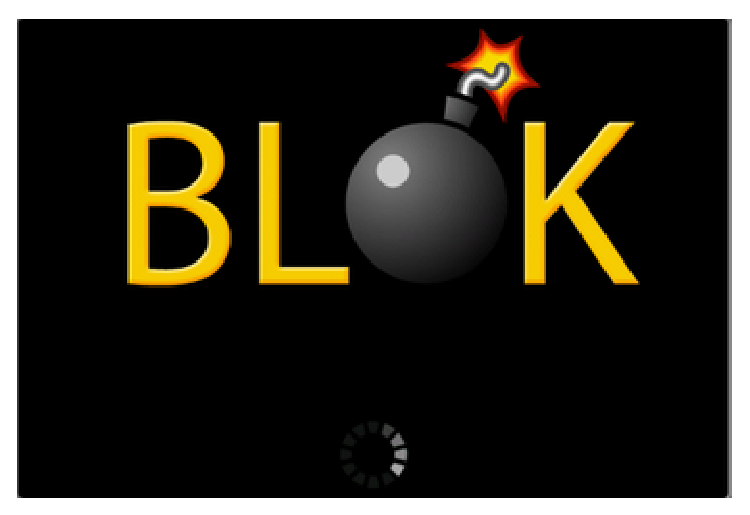
\includegraphics[scale=0.6]{Developpement/Img/1.eps}
		\end{center}
	Une fois ces étapes réalisées, les cartes du jeu vont être copiées dans
	le répertoire du téléphone. Celles-ci seront des cartes officielles permettant
	de jouer dès le premier lancement.
	
	\subsubsection{Création utilisateur}
	Dès lors que toutes ces initialisation sont achevées avec succès, la page de
	création de compte local est enfin affichée.
		\begin{center}						
			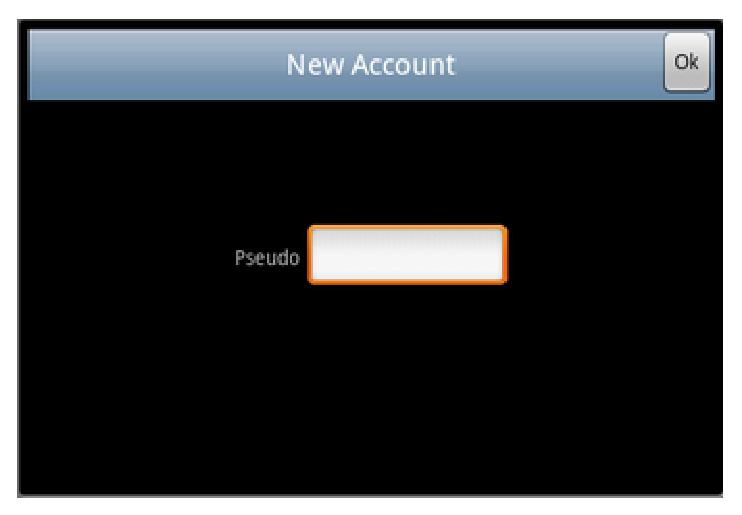
\includegraphics[scale=0.6]{Developpement/Img/2.eps}
		\end{center} 
	Ce dernier est obligatoire afin de pouvoir utiliser l'application. L'utilisateur renseigne son pseudonyme
	pour son profil, qui est ensuite inséré dans la base de données.
	Le menu principal apparait alors.
	\begin{center}						
			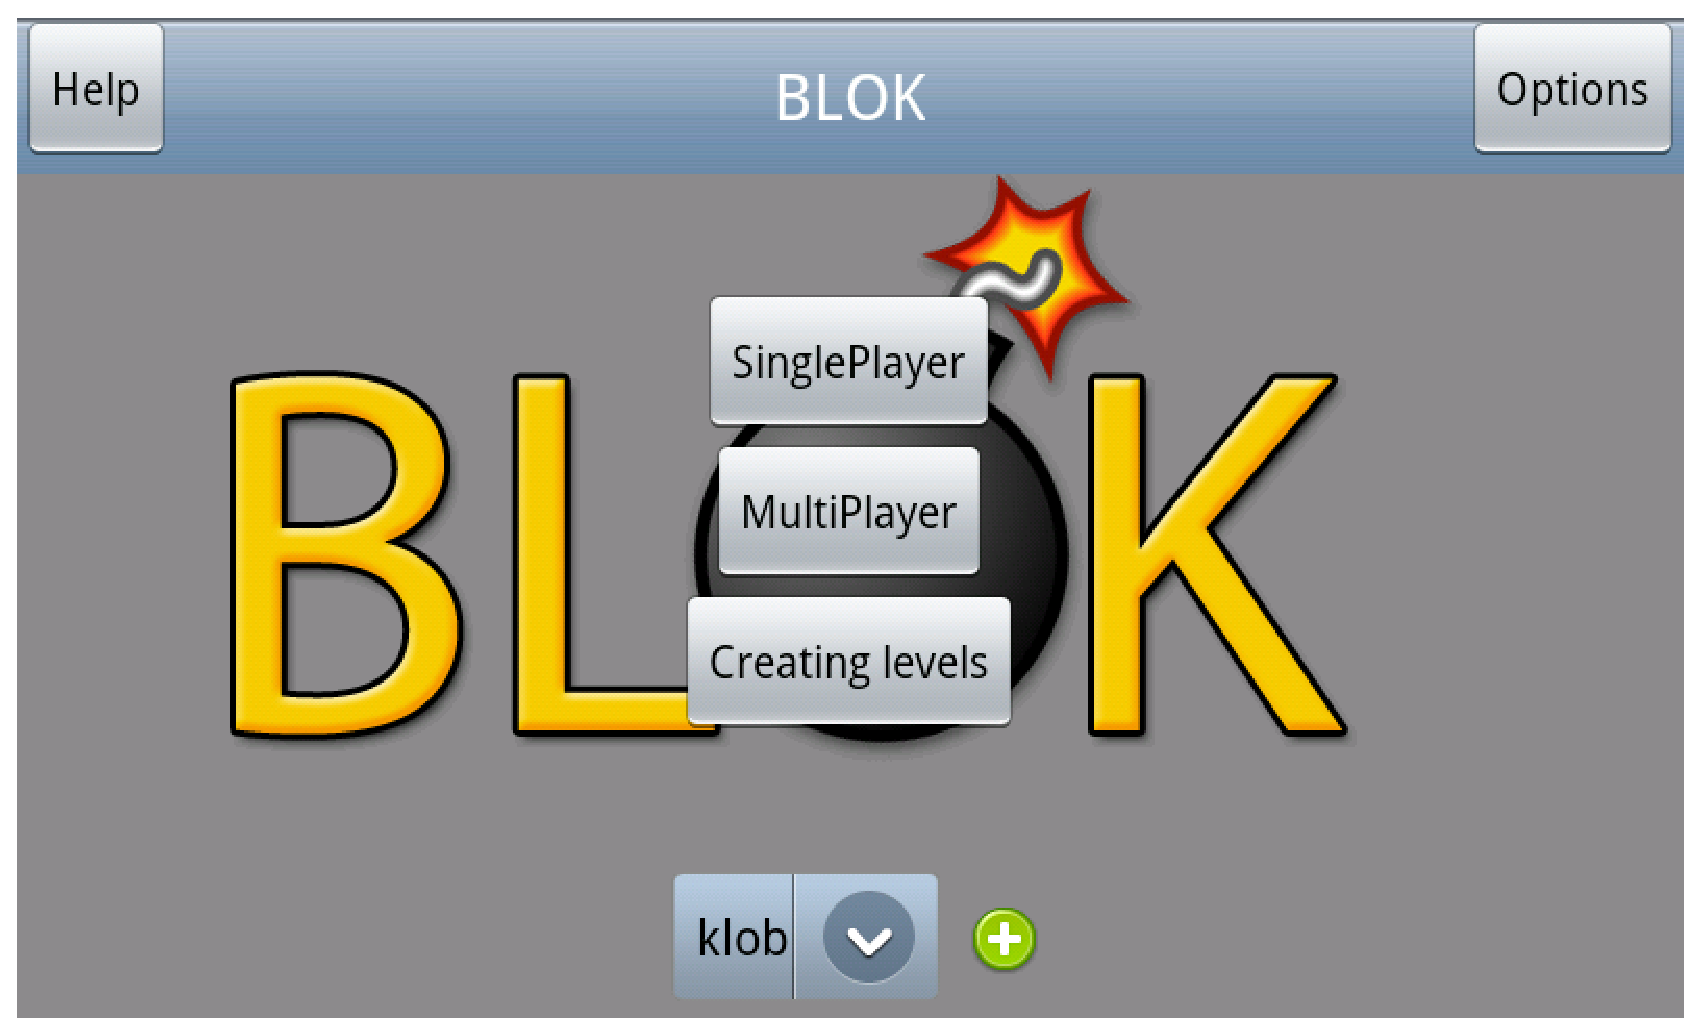
\includegraphics[scale=0.3]{Developpement/Img/3.eps}
		\end{center} 
	
	\subsubsection{Gestion utilisateur}
	A tout moment l'utilisateur a la possibilité d'éditer son profil, qu'il
	soit local ou multijoueur. Cette gestion est une section du menu Option.
		\begin{center}						
			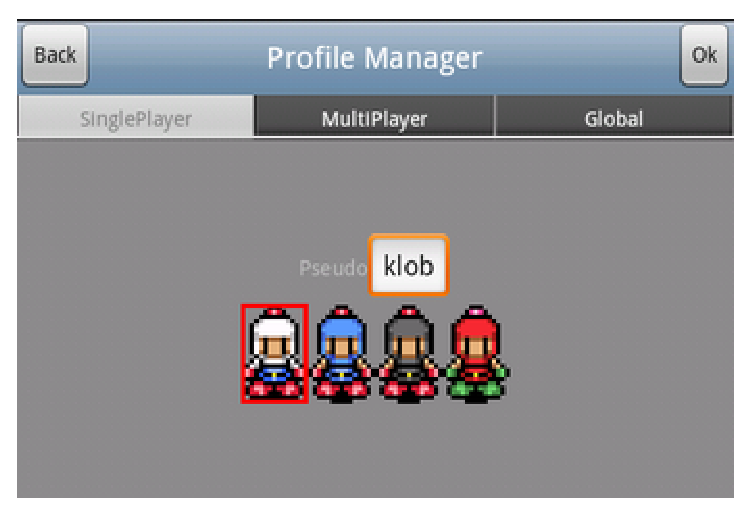
\includegraphics[scale=0.6]{Developpement/Img/5.eps}
			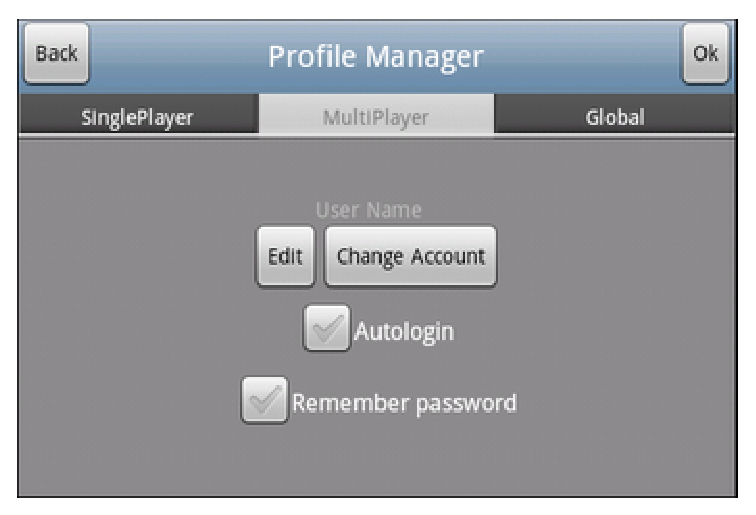
\includegraphics[scale=0.6]{Developpement/Img/6.eps}
		\end{center}
	Pour le profil local il pourra changer de pseudonyme, tout en respectant l'unicité de
	ce dernier dans la base de données, ainsi que de choisir sa couleur de
	personnage. Pour finir il aura le choix de positionner le menu à sa
	guise, suivant qu'il soit gaucher ou droitier.
	
	\subsubsection{Gestion des préférences système}
		\begin{center}						
			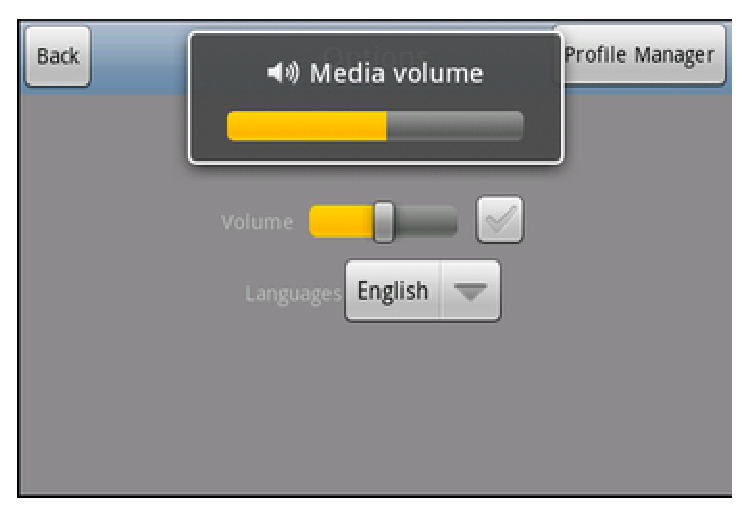
\includegraphics[scale=0.6]{Developpement/Img/4.eps}
		\end{center}
	Grâce au menu d'Option, l'utilisateur peut
	modifier le son de l'application ainsi que la langue utilisée dans cette
	dernière.
	
	\subsubsection{Création de carte}
	La création de carte est une fonctionnalité plus qu'interessante puisqu'elle
	vous permet comme son nom l'indique de créer vos propre cartes et de jouer
	dessus. Vous n'aurez pour cela qu'a renseigner un nom de carte non existant. 
	\begin{center}						
			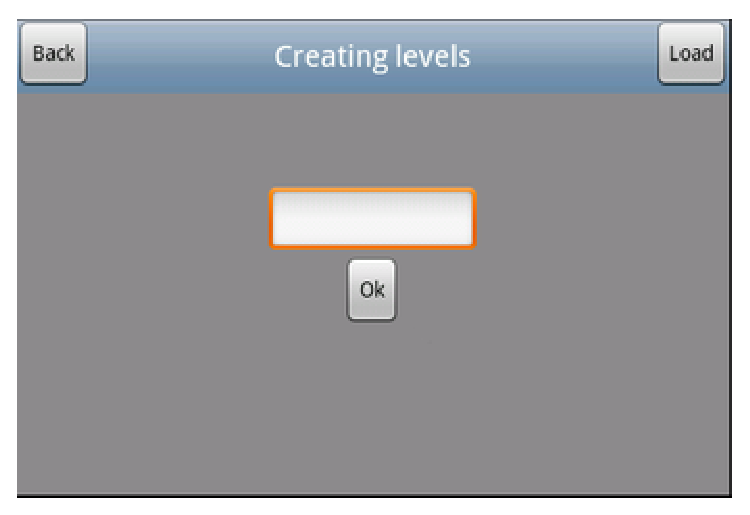
\includegraphics[scale=0.6]{Developpement/Img/10.eps}
			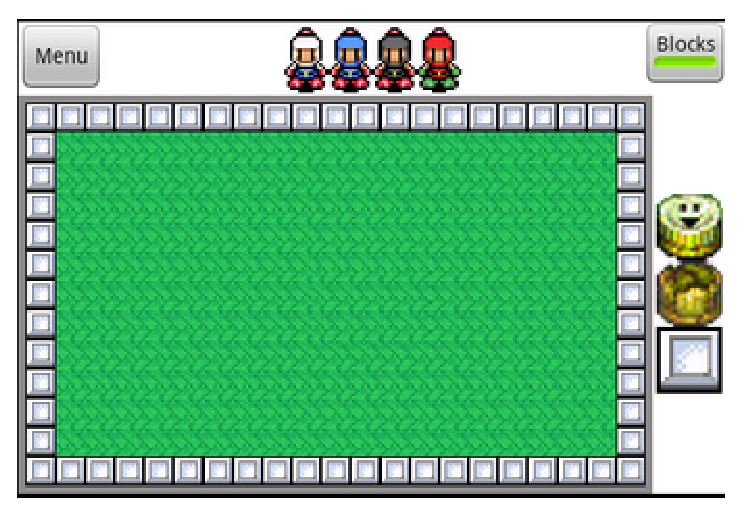
\includegraphics[scale=0.6]{Developpement/Img/11.eps}
		\end{center}
	Il vous sera possible par la suite de les éditer et de les modifier à souhait,
	en laissant libre cours à votre imagination.
	
	
	\subsubsection{Création partie solo}
	La section la plus interressante concerne bien évidement la création de parties
	locales. Vous aurez la possibilité de configurer ces dernières suivant vos
	attentes. Cette configuration passe par le choix de la carte de jeu, officielle
	ou préalablement créée, mais aussi la difficulté des adversaires(\gls{bot})
	et leur nombre avec le temps de jeu.
		\begin{center}						
			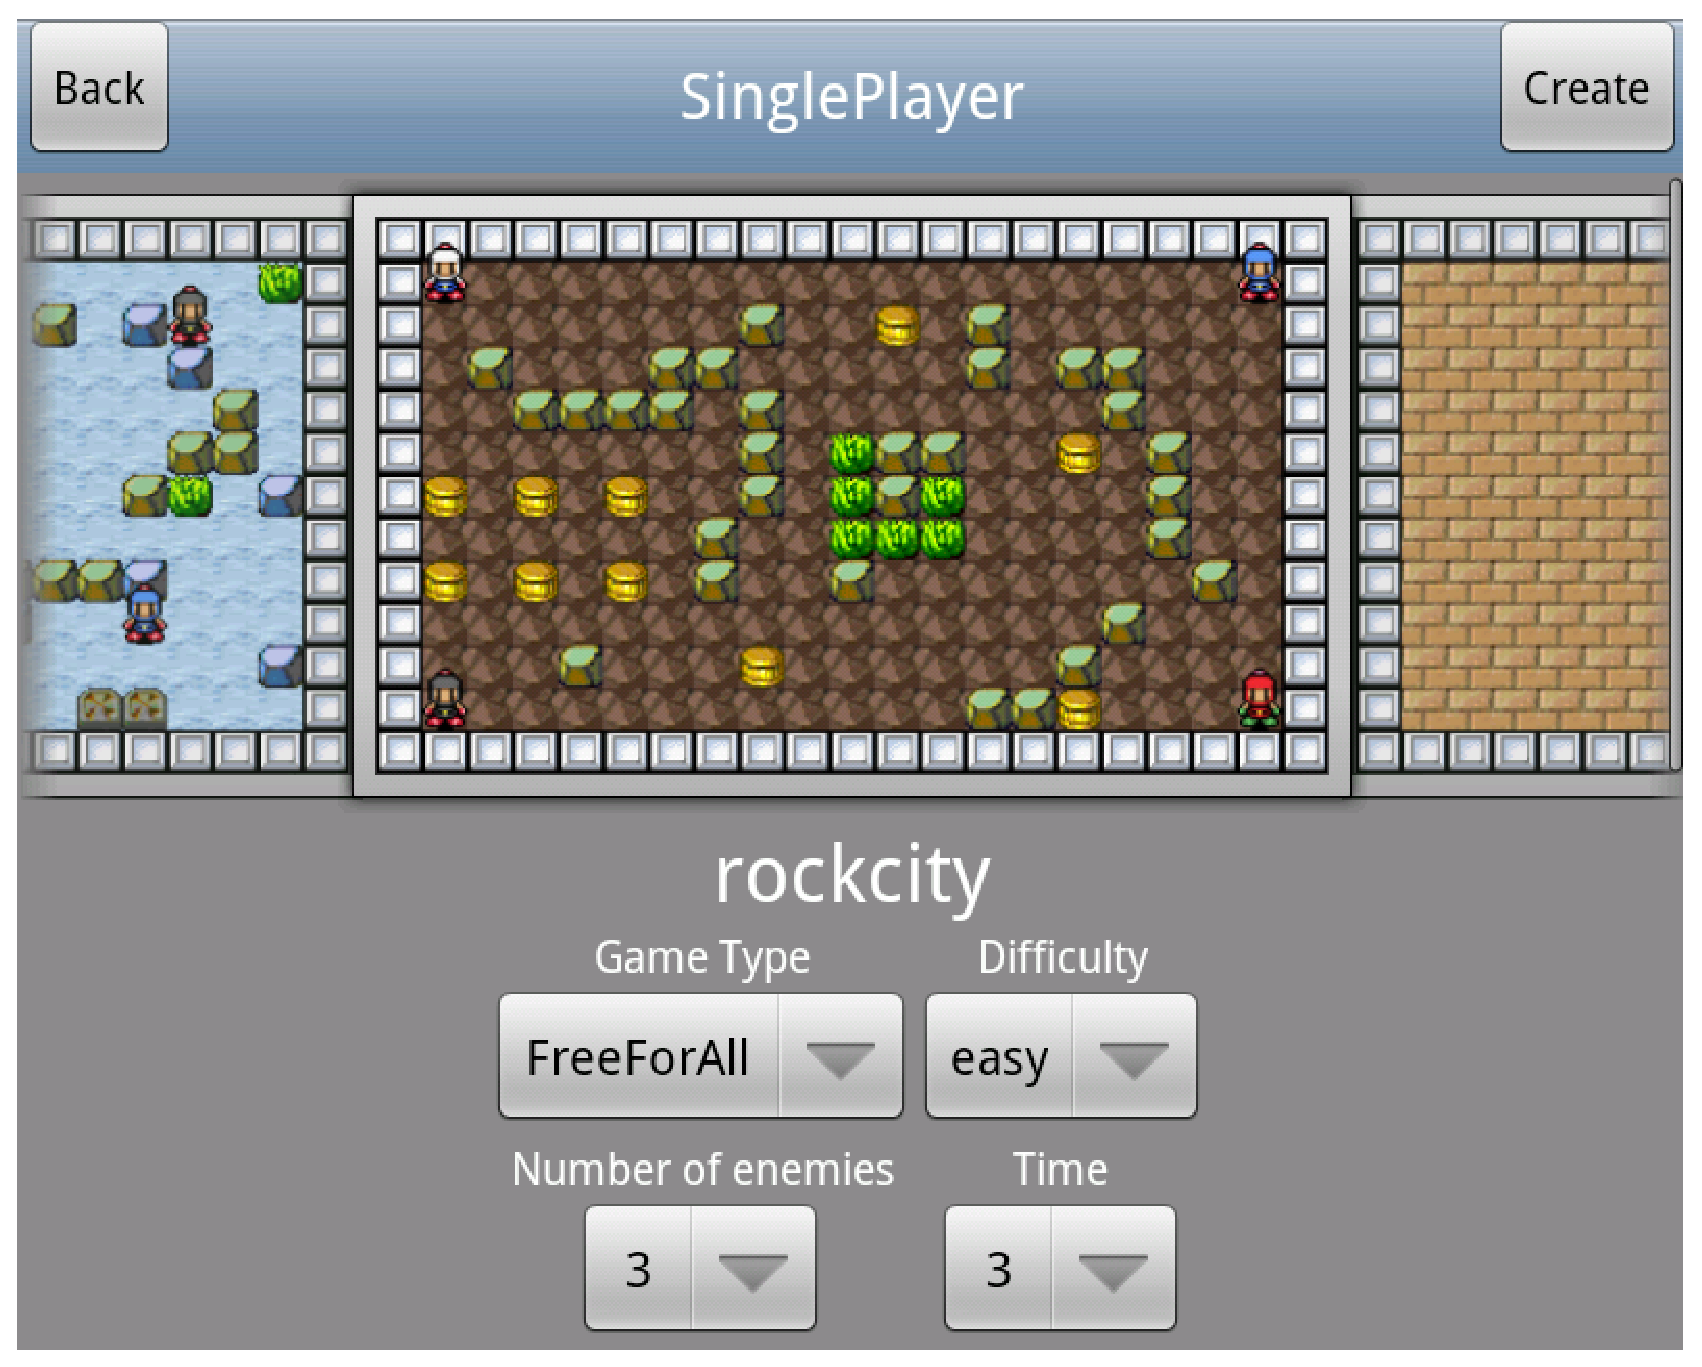
\includegraphics[scale=0.4]{Developpement/Img/7.eps}
		\end{center} 
	Enfin le type de partie souhaité est lui
	aussi inclus dans les paramètres de jeu. Une fois vos préférences choisies
	vous n'aurez plus qu'à lancer la partie, qui débutera quelques instants après.
	
	
	\subsubsection{Création partie multi}
	Cette section est très proche de la création de parties locales. La seule
	différence notable concerne le choix du nombre d'adversaire. Puisqu'il s'agit
	de parties multijoueurs, les adversaires ne seront pas des \gls{bot} mais bel
	est bien des humains. 
	Là encore dès que vos choix de configurations seront faits, vous pourrez
	choisir de créer la partie. Cette dernière s'initialisera sur le serveur, et ne
	débutera que lorsque le nombre de joueurs requis sera complété. Une page
	d'attente vous sera alors affichée.
	
			

\subsection{Editeur de carte}

	\hypertarget{Editeur de carte}{}
	\label{Editeur de carte}
	
	\subsubsection{Général}
		\paragraph{Moteur de rendu\\}
			Pour modéliser la carte que le joueur est en train de construire, nous avons décidé de la représenter sous forme de deux matrices. 
			
			Tout d'abord la matrice contenant tous les éléments représentant le sol.
			\begin{center}
				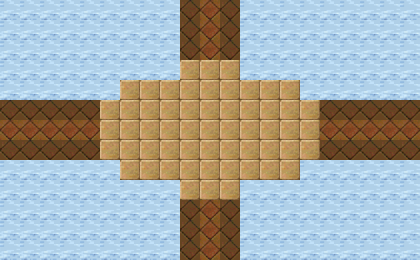
\includegraphics{./Developpement/Img/image1.png}
			\end{center}
			Cette première matrice sera déssinée en premier sur la carte.
			
			Ensuite, la deuxième matrice sera déssinée au dessus de la précédente. Elle contient tous les blocs du décor avec lesquels les joueurs pourront intéragir. 
			\begin{center}
				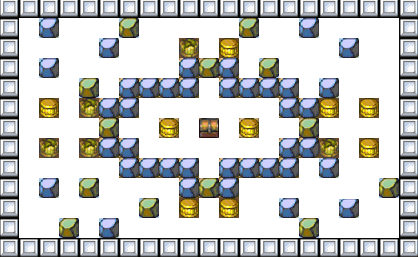
\includegraphics{./Developpement/Img/image2.png}
			\end{center}
			
			Grâce à ces deux matrices, les joueurs pourront à tout moment modifier les éléments de la première ou de la deuxième.
			
			En fusionnant ces deux matrices, nous obtenons la carte compléte.
			\begin{center}
				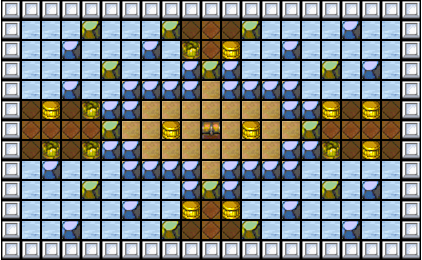
\includegraphics{./Developpement/Img/image3.png}
			\end{center}
			

	\subsubsection{Le modèle}
		La carte est la principale information que l'éditeur de carte doit gérer. Pour représenter une carte, nous avons choisi de la représenter sous la forme de deux matrices ayant les mêmes dimensions que la carte. La première matrice contient des \textit{Object} représentant le sol et la deuxième contient elle aussi des \textit{Object} mais ces derniers représentent des blocs et non le sol. Pour gérer les deux matrices nous avons utilisé des \textit{NSMutableArray} qui sont des tableaux Objective-C que l'on peut modifier, ils contiennent eux aussi des \textit{NSMutableArray} car il n'existe pas des constructeurs de matrice comme en JAVA. Ensuite l'autre information que la carte doit possèder c'est la position de départ des joueurs. Nous avons utilisé un \textit{NSMutableDictionary} permettant de faire la liaison entre la couleur du joueur et son point de départ. 
			
		Lorsque l'utilisateur à terminé de créer ça carte, il a besoin de la sauvegarder. Pour cela nous avons donc utilisé la sérialisation des objets. Lors de l'enregistrement de la carte un fichier \og .klob \fg  est généré. Ce dernier contient les informations nécessaires pour la reconstruction de la carte. Pour reconstruire une carte, il suffit de désérialiser le contenu du fichier \og .klob \fg correspondant. Pour utiliser la serialisation en 
		\gls{objective-c}, nous avons juste besoin
		 implémenter le protocol \textit{NSCoding} qui comporte deux méthode à définir : 
		\textit{- (id)initWithCoder:(NSCoder *)aDecoder} permettant de déserialisé et \textit{- (void)encodeWithCoder:(NSCoder *)aCoder} s'occupant de la serialisation.
	
	\subsubsection{La vue}
		Pour faciliter le développement mais aussi ça réutilisabilité, nous avons découpé la vue de l'éditeur de carte en trois zones. Chaqu'une de ces vues est associée à un contrôlleur qui permet de faire la liaison avec le modèle. Pour concevoir les vues nous avons utilisé la classe UIView qui est prévue pour réaliser une interface graphique sur iPhone. 
			
		\begin{center}
			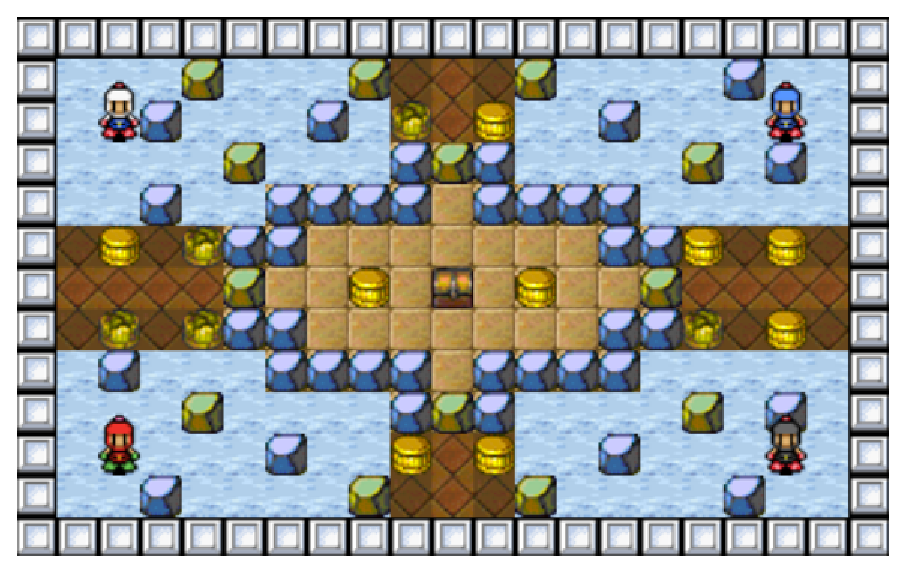
\includegraphics[width=11cm]{./Developpement/Img/carte.eps}
		\end{center}
		Tout d'abord, la vue la plus importante que nous avons créé est la vue affichant la carte. Elle permet au joueur d'intéragir avec celle-ci et de pouvoir créer des cartes selon ses envies. Pour réaliser cette intéraction, nous avons dû surcharger trois methodes de la classe \textit{UIResponder} : \textit{touchesBegan}, \textit{touchesMoved} et \textit{touchesEnded} permettant de gérer tous les évènement générés lorsque l'utilisateur appuiera sur la vue. La methode \textit{touchesBegan} permet de récupérer l'évènement lorsque l'utilisateur va appuyer sur la vue, grâce à cette évènement, on peut savoir à quelle position l'utilisateur à pressé la vue. Ensuite pour récupérer l'évènement lorsque l'utilisateur fais glisser son doigt sur l'écran, il nous suffit d'utiliser \textit{touchesMoved}. Et pour finir lorsque l'utilisateur retire son doigt, nous utilisons la méthode \textit{touchesEnded}. A l'aide de ces trois méthodes, nous avons implémenté les différents gestes que l'utilisateur peut effectuer pour créer une carte. Pour dessiner la carte, nous avons dû surcharger la methode \textit{- (void)draw:(CGContextRef)context}. Celle-ci permet de modifier le comportement de l'affichage de la vue mais elle donne aussi la possibilité de dessiner n'importe quel objet.
		
		\begin{center}
			
\includegraphics{./Developpement/Img/menu_droite.pdf}
		\end{center}
			
		Ensuite, nous avons créé une vue permettant de sélectionner les objets que l'utilisateur peut mettre sur la carte. Cette dernière se trouve à droite de la carte. Dans cette dernière, nous avons des \textit{UIButton} permettant de supprimer des objets ou encore pour changer le type d'objet à placer sur la carte. Mais le plus important de cette vue est la liste déroulante qui permet de choisir l'objet que l'on veut placer sur la carte. Cette liste déroulante n'étais pas un \gls{widget} de base et nous avons donc dû l'implémenter. La particularité de cette liste est qu'elle est générique, ce qui permet de l'utiliser dans plusieurs cas différents, notamment dans les menus pour afficher le choix des cartes. Grâce à celle-ci l'utilisateur peut changer d'objet selectionné en exerçant un simple mouvement vertical du doigt.
			
		\begin{center}
			
\includegraphics[width=11cm]{./Developpement/Img/menu_haut.pdf}
		\end{center}
		Enfin la dernière vue que nous avons réalisé, est une vue contenant plusieurs \textit{UIButton} mais aussi un \textit{UISegmentedControl} qui permet de basculer du mode affichage complet (dessiner tous les éléments de la carte) de la carte, au mode d'affichage partiel (qui affiche que le sol et cache les blocs de la carte) facilitant la modification du sol malgrès les blocs.
			
			
	\subsubsection{Le controlleur}
		
		Le controlleur est une partie très importante de l'architecture \gls{mvc}, elle permet de faire le lien entre les interactions de l'utilisateur sur l'éditeur de carte et les données relatives à celui-ci. Nous avons  donc créé des objets de type \textit{UIViewControler}, ces objets nous ont permis de réaliser cette liaison. Grâce à celle-ci, le modèle et la vue sont complètement indépendants ce qui permet de changer de vue sans avoir besoin de modifier le modèle. Comme nous avons divisé l'éditeur de carte en plusieurs sous vues, nous avons donc créé un contrôlleur pour chacune d'entre elles. Chacun de ces contrôlleur possède eux-même un contrôleur global qui sera le seul à contacter diréctement le modèle. Lorsqu'un utilisateur va réaliser une action dans la vue de l'éditeur de carte, cette dernière va appeler une methode de son contrôleur directe, qui lui appelera une methode du contrôleur global, qui se chargera d'appeler la bonne méthode du modèle en fonction de l'action effectuée par l'utilisateur. 



\subsection{Jeu}

	\subsubsection{Moteurs}
	
		Au sein d'un jeu vidéo plusieurs types de moteurs sont mis en place.
		Chacun a un travail bien précis.
		Ici nous en trouvons trois au total à savoir un pour le rendu graphique, un
		pour s'occuper des interactions entre objets (que ce soit des joueurs, des bombes ou autres). Et enfin un dernier gérant
		les actions de l'intelligence artificielle.
		Commençons par le moteur de rendu.
	
		\paragraph{Moteur de rendu\\}
		
			\hypertarget{Moteur de rendu}{}
			\label{Moteur de rendu}
		
			Contrairement à celui que nous avons vu dans la section précédente pour
			l'éditeur de carte
			\footnote{
				\hyperlink{Editeur de carte}{Editeur de carte}
				\og voir section \ref{Editeur de carte}, page \pageref{Editeur de carte}.\fg
			}
			le moteur de rendu se doit d'être beaucoup plus léger. En effet le jeu doit
			dans son ensemble rester le plus fluide afin d'offrir à l'utilisateur une meilleure
			experience. Il faut savoir qu'ici en plus de gérer le rendu, l'application
			doit s'occuper de l'intelligence artificielle
			\footnote{
				\hyperlink{IA}{IA}
				\og voir section \ref{IA}, page \pageref{IA}.\fg
			}.
			, des divers sons
			\footnote{
				\hyperlink{Sons}{Sons}
				\og voir section \ref{Sons}, page \pageref{Sons}.\fg
			} et des interactions entre objets
			 \footnote{
				\hyperlink{Moteur physique}{Moteur physique}
				\og voir section \ref{Moteur physique}, page \pageref{Moteur physique}.\fg
			}..
			qui seront gérés en cours de partie.		
			
			$\,$	
			
			L'utilisateur ne pourra plus modifier la carte et sera
			entièrement dépendant du moteur physique\footnotemark[3]. Par
			exemple un bloc indestructible sera présent tout au long de la
			partie et ne pourra pas être supprimé, il n'est donc plus necessaire de
			savoir quel type de sol se trouve dessous. De plus comme celui-ci ne peut pas
			être détruit et qu'il n'est pas animé son état sera toujours le même et ne
			correspondra qu'à une seule et unique image.
			
			$\,$			
			
			Un autre exemple est celui d'un sol inanimé tel que l'herbe. Dans le cas où
			il n'y a aucun bloc (destructible) au dessus en début de partie, il en sera
			de même à la fin. Il ne nous est pas nécessaire à chaque
			rafraichissement de regarder si un bloc existe dessus. Ce test se fait en
			début de partie est sera valide jusqu'à la fin de celle-ci.
			
			
			Cette remarque s'applique sur tous les objets dits \emph{non animés} dont
			l'état ne changera jamais au cours du jeu et seulement eux.
			
			
			Si l'on avait eu un sol animé représentant de l'eau, il aurait été composé de
			plusieurs images et aurait donc necessité un rafraichissement constant.

			$\,$
			
			Concrètement ce que nous faisons ici à chaque début de partie est de créer
			une image vierge qui aura la taille de la carte affichée sur l'écran dans
			laquelle nous dessinerons tous les objets \emph{non animés}.
			
			$\,$
			
			Pour cela nous allons parcourir les deux matrices définies dans l'éditeur de
			cartes\footnotemark[2] et regarder s'il existe un bloc, si oui est-ce
			qu'il est destructible ?
			
			Si ce bloc est destructible alors il nous est obligatoire de savoir ce qui se
			trouve en dessous.
			Nous allons donc stocker ce bloc dans une table de hachage dont les clefs sont les
			coordonnées de l'objet et dont la valeur est l'objet lui même, et dessiner le
			sol sur l'image citée au dessus.
			
			Si ce bloc est indestructible alors inutile de mémoriser le sol se trouvant
			au dessous.
			
			Sinon s'il n'existe pas de bloc nous allons regarder si le sol est animé. Si
			tel est le cas, alors nous le stockons dans la table de hachage comme un bloc
			destructible, sinon nous le dessinons dans l'image comme un objet inanimé.
			
			$\,$
			
			Voici un exemple concret de la méthode décrite au dessus :
				

			\begin{figure}[!h]			
				\begin{center}			
					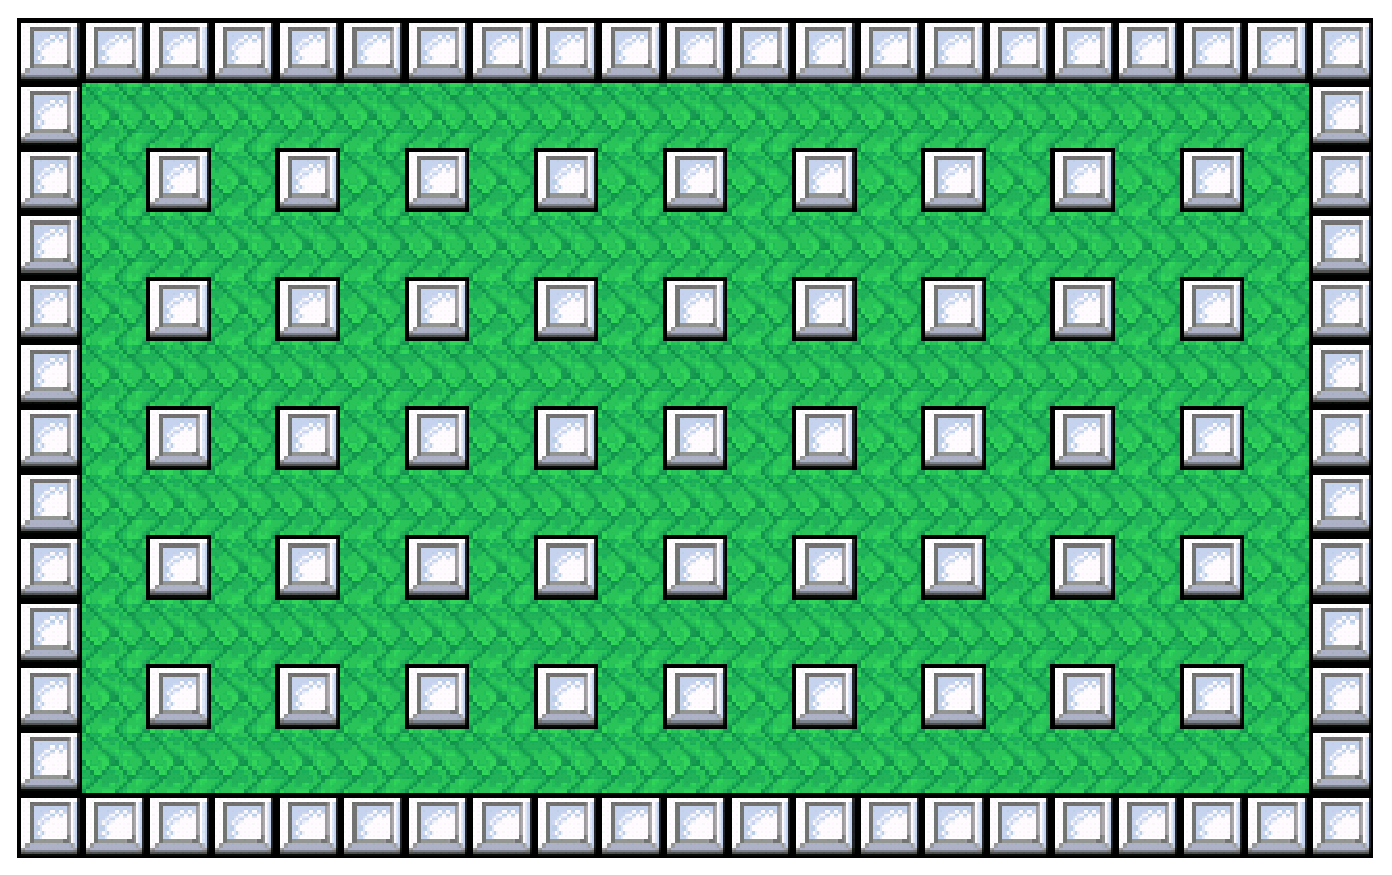
\includegraphics[width=229px, height=142px]{Developpement/Img/map.eps}
					\caption{L'image représentant la totalité des objets non animés}
				\end{center}
			\end{figure}
			
			$\,$			

			\begin{figure}[!h]			
				\begin{center}						
					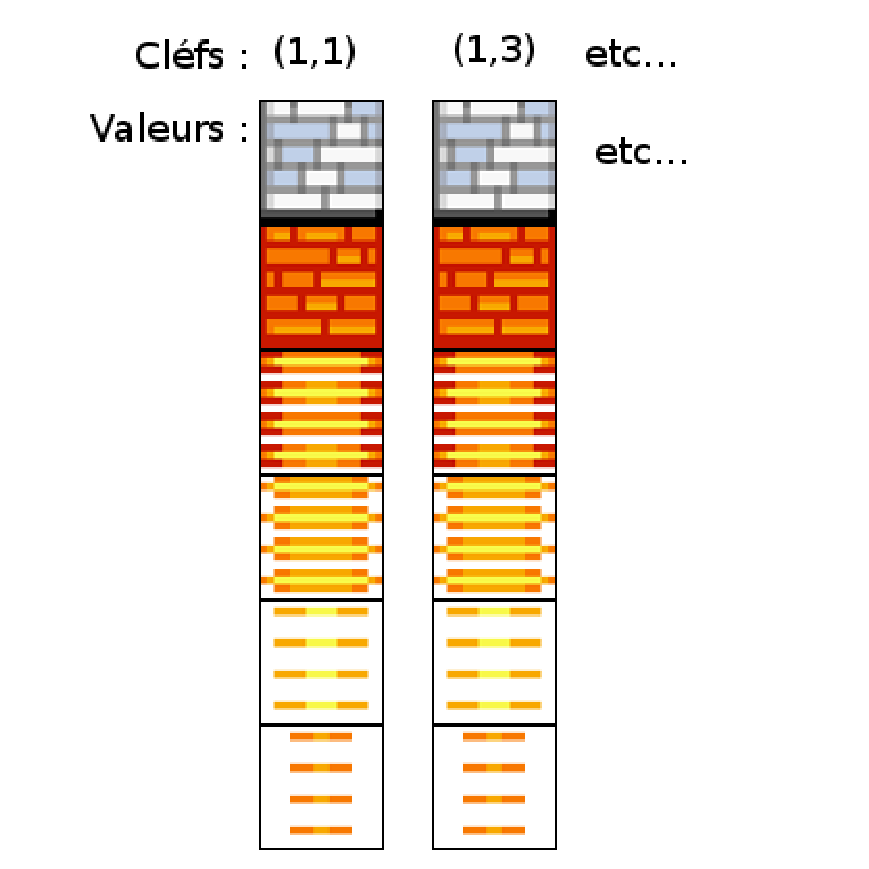
\includegraphics[width=250px, height=250px]{Developpement/Img/hashmap.eps}
					\caption{La hashmap des objets animés}
				\end{center}
			\end{figure}

			$\,$
			
			\newpage

			Les avantages d'avoir utilisé une telle structure sont les suivants. Ici au
			lieu de parcourir les 21*13*2 cases des deux matrices à chaque rafraichissement
			(c'est à dire toutes les 50 millisecondes environ) et d'afficher au minimum
			21*13 objets pour le sol et 64 objets pour les bordures si la carte est vide
			(donc énormement plus si il existe d'autres objets), nous n'affichons qu'une
			image plus au maximum 197 objets.
			
			\begin{center}
				\begin{tabular}{|c|c|c|} \hline
				\multicolumn{3}{c}{Compléxité en nombre d'objet à afficher} \\\hline
				  & Editeur de carte & Jeu    \\\hline 
				Meilleur des cas & 337 & 1    \\\hline
				Pire des cas     & 534 & 229  \\\hline		
				\end{tabular}
			\end{center}
			
			Le meilleur des cas ici décrit une carte vide donc composée que de sol non
			animé ansi que des bordures de la carte. Cela représente dans le nouveau
			moteur de rendu une seule et unique image contrairement à l'ancien où chaque
			objet étant affiché indépendament, ce qui était équivalent à 337 objets.
			
			$\,$
			
			Le pire des cas est une carte remplie au maximum de bloc destructibles,
			obligeant dans les deux cas à connaitre le type de sol se trouvant dessous.
			
			$\,$
			
			Nous voyons très clairement les différences de coûts entre les deux méthodes
			de rendu et l'optimisation qu'engendre la deuxième.
			
			De plus ici l'utilisation de la table de hachage permet dans un premier temps de
			retrouver directement un objet de par ses coordonnées, mais aussi de ne pas
			avoir à parcourir $n$ cases vides comme lors de l'utilisation des matrices.
			Au fur et à mesure de la partie il existera de moins en moins d'objets,
			donc garder une structure aussi grosse qu'une matrice n'est pas optimal.
		
		\paragraph{Moteur physique\\}
		
			\hypertarget{Moteur physique}{}
			\label{Moteur physique}
			
			Un moteur physique est, en informatique, une bibliothèque logicielle 
			indépendante appliquée à la résolution de problèmes de la mécanique
			classique.  Les résolutions typiques sont les collisions, la chute des corps,
			les forces, la cinétique, etc.
			Les moteurs physiques sont principalement utilisés dans des simulations 
			scientifiques et dans les jeux vidéos.
			
			
			Ici notre moteur physique se contentera simplement de s'occuper des diverses
			collisions qu'auront les joueurs avec l'environnement les entourant. Mais
			aussi les intéractions qu'auront les divers objets du décors entre eux
			ainsi qu'avec les joueurs.

			$\,$		
			
			Tout comme le moteur de rendu
			\footnote{
				\hyperlink{Moteur de rendu}{Moteur de rendu}
				\og voir section \ref{Moteur de rendu}, page \pageref{Moteur de rendu}.\fg
			}
			le moteur physique d'un jeu doit être optimal dans les traitements qu'il doit
			effectuer, étant donnée son utilisation permanente au cour du jeu.
			
			
			Afin d'optimiser ces traitements lors des collisions nous avons fusionné les
			deux matrices présentent dans l'éditeur de cartes
			\footnote{
				\hyperlink{Editeur de carte}{Editeur de carte}
				\og voir section \ref{Editeur de carte}, page \pageref{Editeur de carte}.\fg
			}
			afin de n'en obtenir qu'une seule reprenant le principe décrit dans le moteur
			de rendu\footnotemark[2].
			
			$\,$
			
			Cette matrice est composée de sept types d'objets différents à savoir :
			
			\begin{center}
				\begin{tabular}{|c|c|} \hline
				Objet  & Description \\\hline
				EMPTY  & Zone vide représentant un sol quelconque\\\hline
				BLOCK  & Un bloc \\\hline
				GAPE   & Un trou \\\hline
				DAMAGE & Une zone de dommages (piques, lasers, etc \ldots) \\\hline
				DANGEROUS\_AREA & Une zone dangereuse\\\hline
				BOMB & Une bombe\\\hline
				FIRE & Feu résultant de l'explosion d'une bombe\\\hline
				\end{tabular}
			\end{center}
			
			Les zones dangereuses sont les zones qui seront touchées lors de l'explosion
			d'une bombe. Ces zones sont spécifiques à l'intelligence artificielle et leur
			permettent de savoir si elles sont en danger ou non.
			
			
			$\,$
			
			Cette matrice est mise à jour lors de la pose et de l'explosion d'une bombe.
			
			De cette façon il est rapide de savoir si un joueur rentre en collision avec
			un objet quelconque ou si celui-ci subit des dommages.
			
			\subparagraph{Exemple}
			
				\begin{itemize}
				  \item Carte originale :
				  
						\begin{center}						
							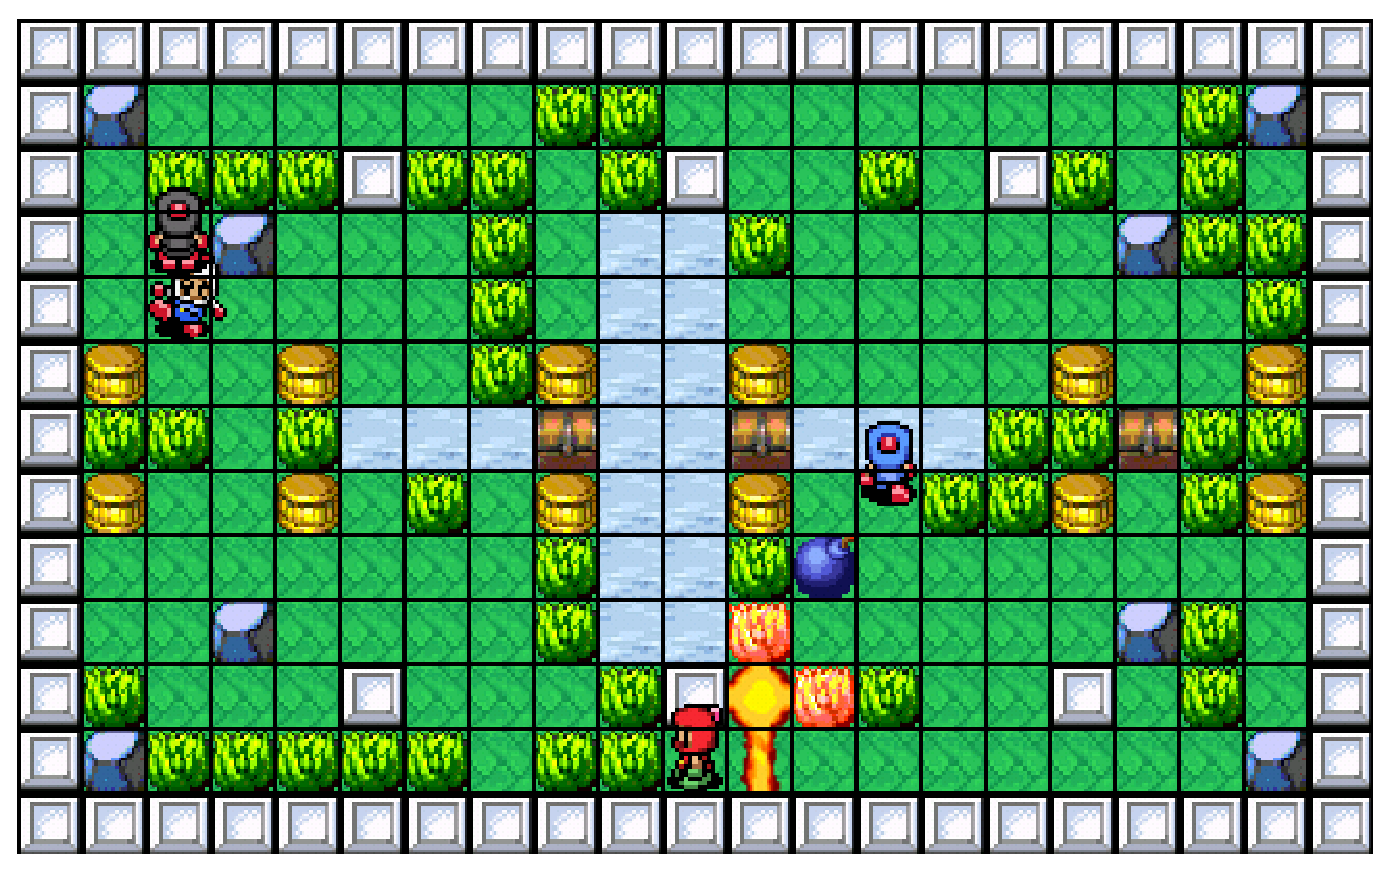
\includegraphics[width=115mm,height=71mm]{Developpement/Img/mapcolision_1.eps}
						\end{center}				  		
				  
				  \item Carte de collision :
				  
						\begin{center}						
							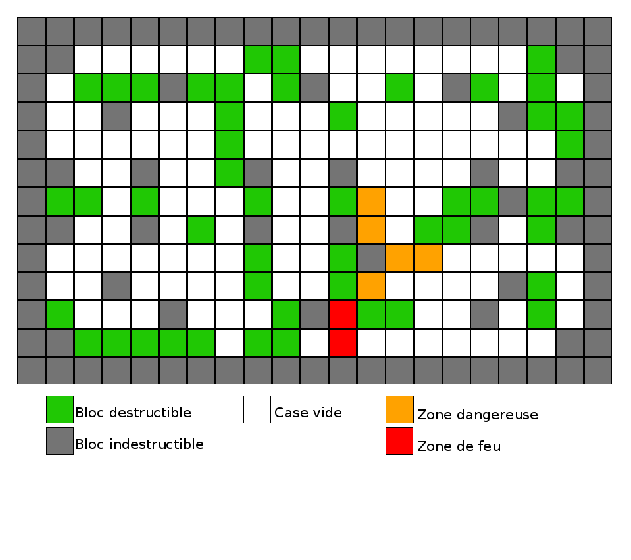
\includegraphics[width=115mm,height=102mm]{Developpement/Img/mapcolision_2.eps}
						\end{center}
						
				\end{itemize}
		

			\subparagraph{Deplacements\\}
			
				$\,$
			
				Globalement la gestion des mouvements est identique sur Android comme sur
				iOS.
				Elle consiste à poser le doigt sur l'écran et à le faire glisser dans la
				direction souhaitée. Ainsi le personnage avancera jusqu'à ce que le doigt
				soit relevé.				
				
				Quant à la gestion des collisions bien que chaque équipe utilise la matrice
				décrite ci dessus, les façons de concevoir la chose ont divergé amenant à
				l'élaboration de deux méthodes de rendu. Dans chacune le joueur se deplace
				verticalement, horizontalement ainsi qu'en diagonale.
				
				\begin{enumerate}
				  \item Collisions sous Android
				  
				  		Le principe de collisions sous Android a été conçu de manière à faire
				  		``glisser'' ou non le joueur lorsqu'il rencontre des obstacles.
				  		
				  		
				  		Pour cela nous allons étudier un mouvement qui sera celui vers le haut
				  		afin de mieux comprendre ce terme.
				  		Nous aurions pu prendre n'importe quel autre mouvement cela serait
				  		revenu au même point.
				  		
				  		Il faut juste retenir qu'au mieux le joueur est dans une case et au pire
				  		dans deux et non dans quatre. En effet lors d'un déplacement nous
				  		n'allons regarder que la face correspondant à cette direction comme le montre
				  		l'image ci-dessous:
				  		
				  		$\,$
				  		
						\begin{center}						
							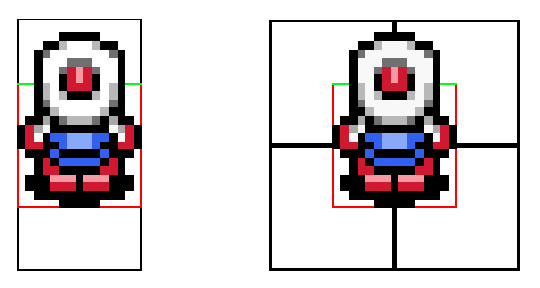
\includegraphics[width=168px,height=84px]{Developpement/Img/ex2.eps}
						\end{center}
						
				  		$\,$				  		
				  		
				  		Le trait vert représente le côté que nous étudierons lors d'un
				  		déplacement vers le haut.
				  		
				  		
				  		Nous partons du principe qu'il n'y a pas de vérification à faire tant
				  		que le joueur ne change pas de case, car du moment où il y est entré
				  		c'est qu'elle est entièrement traversable.
				  		
				  		Il existe donc quatres types de collisions possibles :
				  		
				  		\begin{enumerate}

				  		  \item Le premier cas correspond à celui où les cases sont
				  		  traversables, il n'y a donc qu'à déplacer le joueur vers le haut.

							\begin{center}						
								
\includegraphics[width=168px,height=84px]{Developpement/Img/ok2.eps}
							\end{center}

				  		  \item Le second est celui où la ou les cases en face sont des murs, il
				  		  n'y a alors rien à faire, le personnage ne bouge pas.
				  		  				  		  
				  		  	\begin{center}						
								
\includegraphics[width=168px,height=84px]{Developpement/Img/ko2.eps}
							\end{center}
							
				  		  \item C'est à partir de ce cas que l'on rencontre le glissement cité
				  		  plus haut.
				  		  Ici nous le joueur essaie de monter mais la case de gauche correspond à un
				  		  mur. Etant donné la petitesse des écrans et la rapidité à laquelle le
				  		  jeu se déroule il serait embêtant pour l'utilisateur de devoir se
				  		  décaler à droite de façon à être bien en face de la case libre.
				  		  Nous avons donc pris en compte le cas où le joueur aurait dépassé la
				  		  moitié du bloc intraversable. Dans ce cas là nous le faisons glisser
				  		  sur la droite de façon à ce que celui-ci se place convenablement en
				  		  face de la case et monte normalement.
				  		  
				  		  	\begin{center}						
								
\includegraphics[width=84px,height=84px]{Developpement/Img/ko3.eps}
							\end{center}
				  		  
				  		  \item Le dernier cas est l'opposé du précédent et fonctionne de la
				  		  même manière.
				  		  
				  		  	\begin{center}						
								
\includegraphics[width=84px,height=84px]{Developpement/Img/ko4.eps}
							\end{center}
				  		  
				  		\end{enumerate}

				  
				  \item Collisions sous iOS
				
				Le principe des collisions sous \gls{ios} a été réfléchi de manière a ce que les
				déplacements soient fluides et que les collisions avec des blocs ne
				freinent pas la fluidité du jeu. Car en effet lors des collisions, 
				si le joueur doit passer entre deux blocs, 
				celui-ci doit passer au pixel prêt. Cela implique que l'utilisateur doit
				être très minutieux dans ses déplacements et cela rend le jeu casiment
				injouable lors de passage entre deux blocs. 
				Donc pour remédier à ce problème nous avons décidé d'établir un système de marge sous \gls{ios}.
				C'est à dire que lors de la collision avec un bloc. 
				On va vérifier si au moins un pixel du joueur touche au moins un pixel du
				bloc moins une marge. 
				Voici le tout en image:

				Il faut donc que le rectangle rouge entourant 
				le joueur ne touche aucun autre rectangle rouge entourant
				les blocs, pour que le joueur puisse se déplacer. Les rectangles délimitant
				les blocs sont réduits grâce à la marge (fleche jaune) pour permettre à
				l'utilisateur de passer facilement.
				
				$\,$
				  		
				\begin{center}						
			%		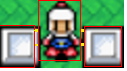
\includegraphics[width=168px,height=84px]{Developpement/Img/mouvementCollision.pdf}
				\end{center}
						
				$\,$	
				
				
				\end{enumerate}
			
			\subparagraph{Gestion des bombes}
				\begin{itemize}
					\item{Threads}
				\end{itemize}
	
	\subsubsection{IA}
	
		\hypertarget{IA}{}
		\label{IA}
		
		\paragraph{Pathfinding}
			\subparagraph{A*}
			\subparagraph{Aléatoire}
			\paragraph{Prise de décision}
			

	\subsubsection{Sons}
	
		\hypertarget{Sons}{}
		\label{Sons}
	
	\subsubsection{Interface utilisaeur}
		\paragraph{Android}
		\paragraph{iOS}

		
		
\section{Serveur}
	
		
%\subsection{JSON}
	
		
\subsection{Servlet}
	
		Comme expliqué précédement notre serveur est conçu grâce aux \glspl{servlet}.
		Après avoir décrit leur fonctionnement, nous allons montrer dans cette partie
		comment elles ont été utilisé.
		
	\subsubsection{En pratique}
		Au lancement du serveur la classe ContextListener est invoquée lorsque l'objet
		ServletContext est crée. Sa méthode contextInitialized(ServletContextEvent event) sera alors appelée, 
		permettant ainsi de définir des objets communs à toutes les
		\glspl{servlet}, tels qu'un accesseur à la base de données, ou le tableau qui
		contenant les utilisateurs connectés. Les requêtes font appel à la fonction
		post des \glspl{servlet}. Le flux entrant étant de type \gls{json}, il faut
		désérialiser le flux dans un objet correspondant. Exemple l'utilisateur envoie son nom d'utilisateur ansi que son mot de passe crypté
		dans un tableau, sérialisé en \gls{json}.
		Pour pouvoir récupérer les informations nous procédons comme suit: 
		
		\begin{verbatim}
			BufferedReader req = 
				    new BufferedReader(new InputStreamReader(request.getInputStream()));
			OutputStreamWriter writer = 
				    new OutputStreamWriter(response.getOutputStream());
			String message = req.readLine();
			
			if (message != null) {
				  response.setContentType("text/html");
				
				   // désérialisation des infos de l'utilisateur dans une arraylist 
				  JSONDeserializer<ArrayList<String>> jsonDeserializer = 
					    new JSONDeserializer<ArrayList<String>>();
				  ArrayList<String> identifiers;
				  identifiers = jsonDeserializer.deserialize(message);
				
				  username = identifiers.get(0);
				  password = identifiers.get(1);
				  
			  ...}
		\end{verbatim}
		
		
	\subsubsection{La sécurité}
	
		Ce serveur de jeu étant hebergé sur internet et contenant des informations
		sensibles d'utilisateurs, tels que des mots de passes, il était crucial
		d'instaurer des règles de sécurité et de cryptage. 
		
		En effet lors des inscriptions ou connexion au serveur pour le mode
		multijoueur, les mots de passes sont tout d'abord cryptés côté client et
		ensuite encapsulés dans un flux \gls{json}, pour être envoyés au serveur. Il
		stockera ainsi la chaine de caractères extraite de l'objet déserialisé. De cette
		manière à aucun moment les données confidentielles ne transiteront en clair.
		
		De plus un mécanisme semblable aux sessions est en place. Dans la
		confirmation de connexion ou d'inscription, une userKey est générée. Elle correspond en
		réalité à l'identifiant de session envoyé par le serveur. Une fois associée
		au nom d'utilisateur correspondant, le tout est ajoûté dans le tableau
		d'utilisateurs connectés.
		Cette userKey est ensuite nécessaire pour contacter les \glspl{servlet}
		suivantes. Si cet identifiant n'est pas envoyé ou n'est pas présent dans le tableau des
		utilisateurs connectés, il sera alors impossible à l'utilisateur d'accéder aux
		ressources du serveur.
		
\subsection{BDD}

	La base de données du serveur n'est pas très complexe. En effet elle ne fait
	qu'accueillir les couples (nom d'utilisateur, password) des utilisateurs dans
	la table Users. 
	Pour son accès, chaque \gls{servlet} peut récupérer un objet de type
	Connection, instancié à l'initialisation du serveur. Il permettra à son tour
	de récuperer un objet de type Statement. L'application va l'employer pour
	transmettre des instructions à la base de données.
	Exemple d'insertion: 
		
	\begin{verbatim}
	Connection connection = 
	  DriverManager.getConnection("jdbc:mysql://127.0.0.1/Bomberklob", "user","user");
	Statement theStatement = connection.createStatement();
	theStatement.execute(
		     "INSERT into Users VALUES ('"+ username +"','"+password+"')");
	\end{verbatim}
	
	Bien évidemment cette adresse est remplacée par une variable, elle aussi
	présente dans le ContextListener, contenant la véritable adresse de la base de
	données.
	
	
	
	

	
		
		
		
\chapter{Manuel d'utilisation}

	\section{Menus}
	

\subsection{Premier lancement}
	
		
\subsubsection{Création compte local}
	Au premier lancement de l'application, il vous est demandé de créer un compte 
	local. Ce dernier est nécessaire pour pouvoir utiliser l'application. Il vous
	suffit de renseigner dans le champs prévu à cet effet, votre pseudonyme (1).
	\begin{center}
			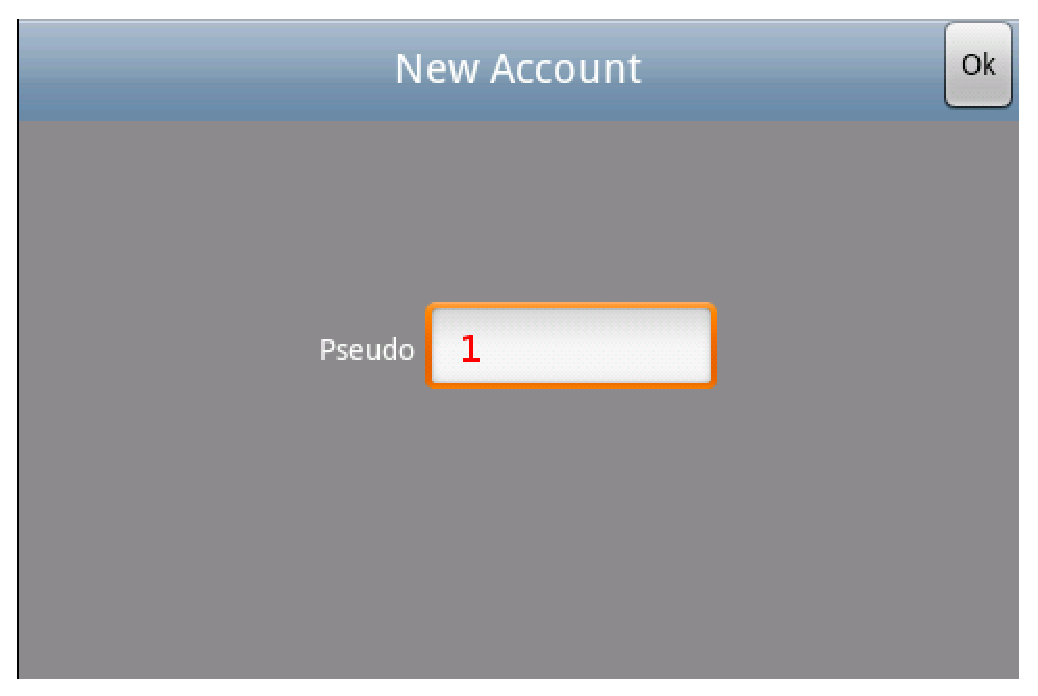
\includegraphics[scale=0.6]{Manuel/Img/2.eps}
	\end{center}


\subsection{Menu principal}
	Le menu d'accueil, vous permet d'accéder à la section des parties locales
	\textcolor{red}{\textbf{1}}, des parties multijoueurs
	\textcolor{red}{\textbf{2}}, l'éditeur de carte \textcolor{red}{\textbf{3}}
	pour créer vos propres cartes de jeu, le menu d'options
	\textcolor{red}{\textbf{4}}, l'accès aux comptes locaux
	\textcolor{red}{\textbf{5}}, la création d'un nouveau compte local
	\textcolor{red}{\textbf{6}} et enfin l'aide \textcolor{red}{\textbf{7}}.
	
	\begin{center}
		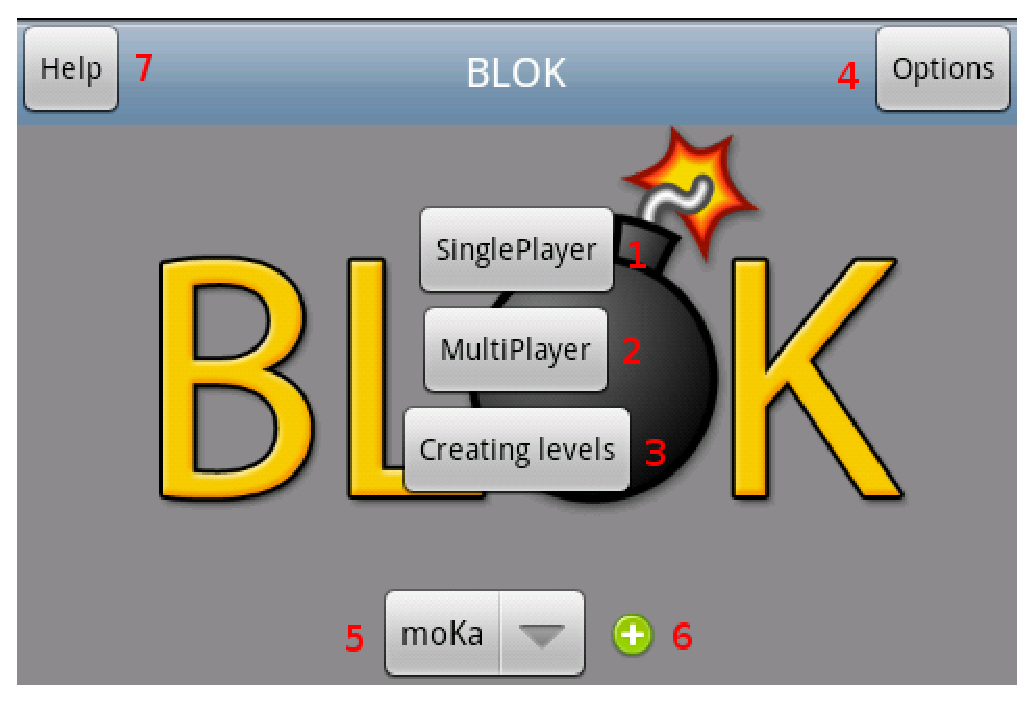
\includegraphics[scale=0.7]{Manuel/Img/3.eps}
	\end{center}
	
	
	
\subsection{Jeu local \textcolor{red}{1}}
	\subsubsection{Paramétrage}
	Voilà un moment crucial précédent votre lancement de jeu, sa configuration.
	Rien de bien compliqué en soit, vous choisissez le type de partie
	\textcolor{blue}{\textbf{2}}, la difficulté de vos des \glspl{bot}
	\textcolor{blue}{\textbf{3}}, le nombre d'ennemis sur la carte
	\textcolor{blue}{\textbf{4}}, le temps de jeu \textcolor{blue}{\textbf{5}},
	et enfin grâce à un défilement de la galerie \textcolor{blue}{\textbf{1}}, la
	carte de jeu. Vous n'avez plus qu'à valider
	\textcolor{blue}{\textbf{7}} ou revenir au menu précédent
	\textcolor{blue}{\textbf{6}}.
	
	\begin{center}
		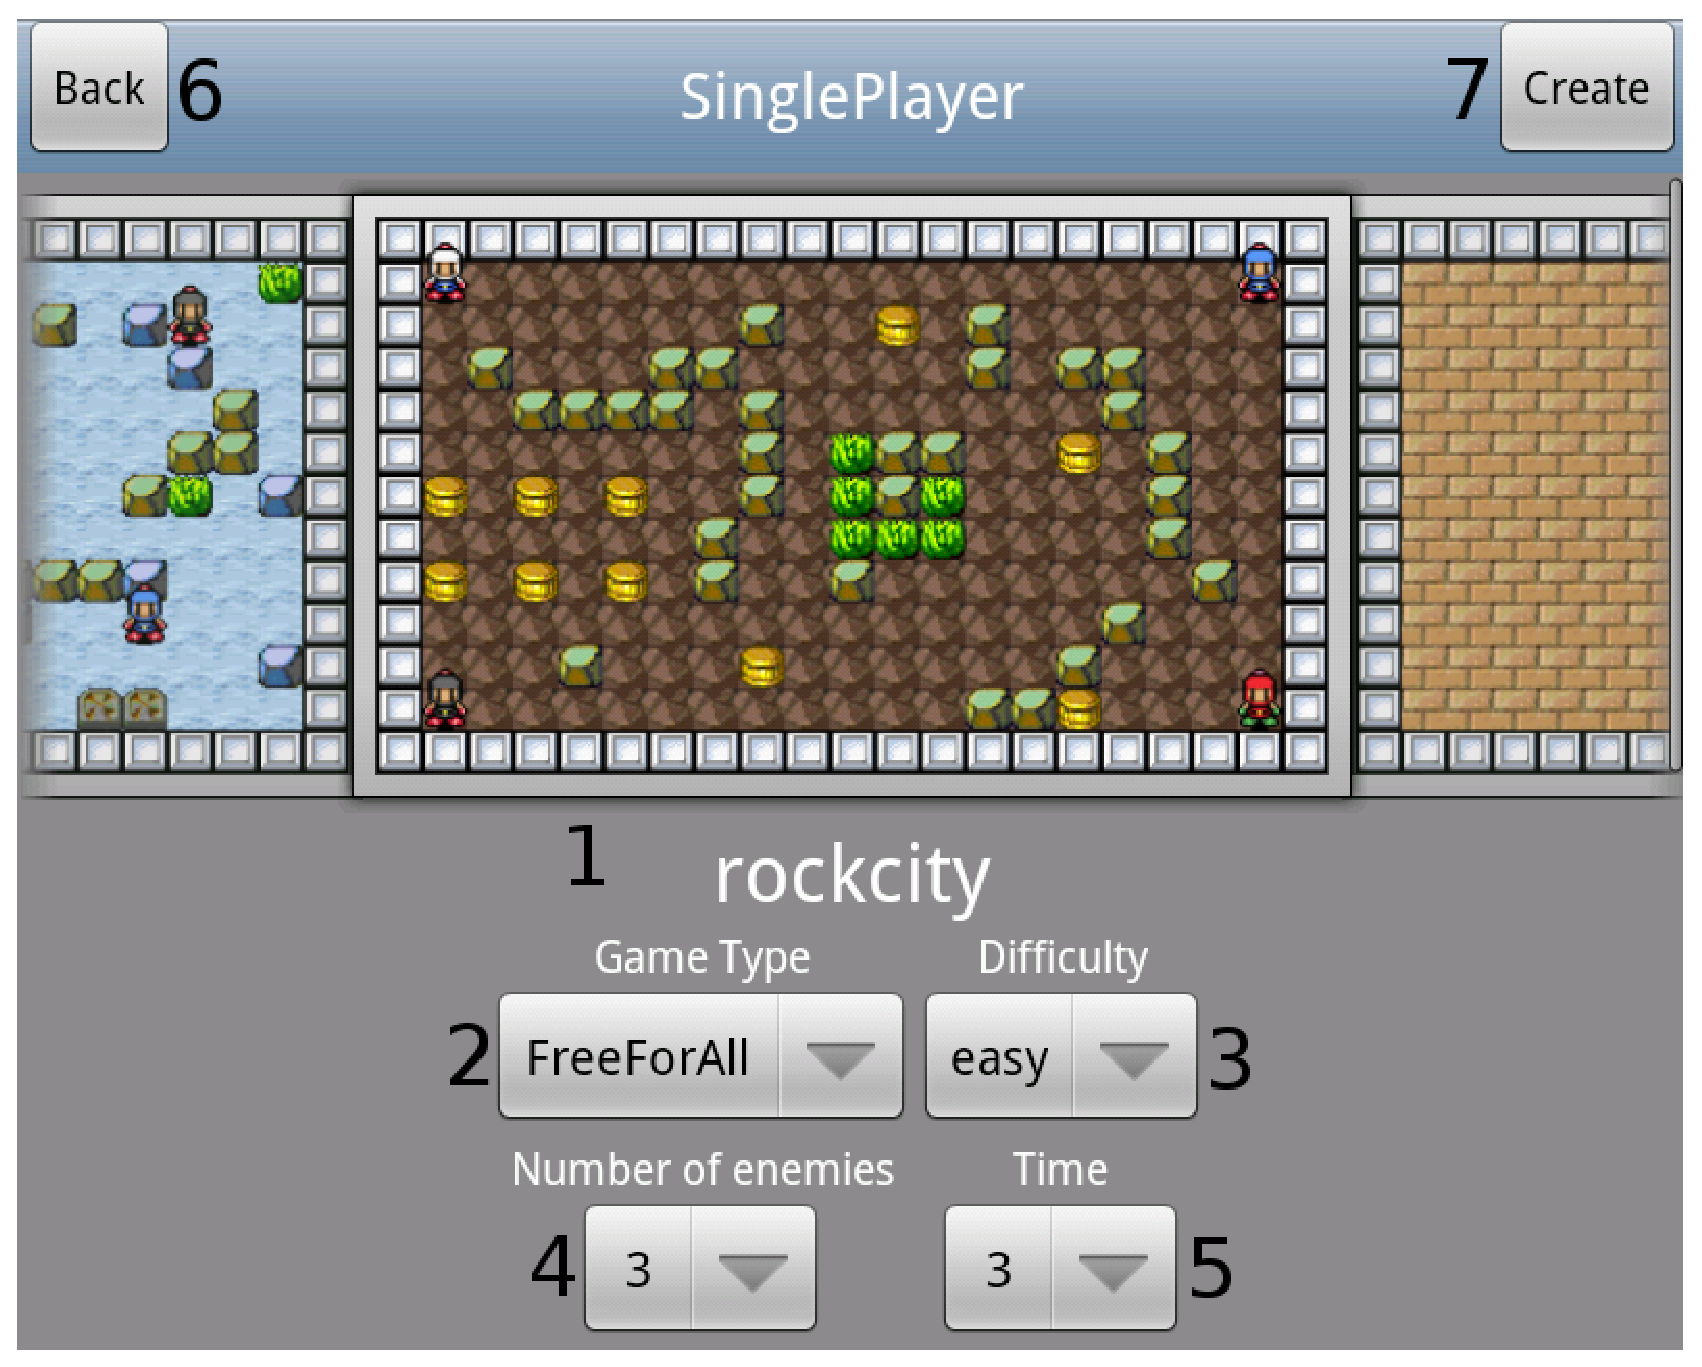
\includegraphics[scale=0.4]{Manuel/Img/15.eps}
	\end{center}
	
	
\subsection{Jeu multijoueur \textcolor{red}{2}}

	\subsubsection{Inscription}
	Cette étape est inévitable afin d'accéder au mode multijoueur. Vous devez
	renseigner le nom d'utilisateur \textcolor{blue}{\textbf{1}}, mot de passe
	\textcolor{blue}{\textbf{2}}, et confirmer ce dernier
	\textcolor{blue}{\textbf{3}}. Vous pouvez choisir une connexion automatique
	\textcolor{blue}{\textbf{4}} ou simplement ne pas ressaisir votre mot de passe
	aux connexions suivantes \textcolor{blue}{\textbf{5}}. Dès que ces champs sont
	remplis, validez via la connexion au serveur \textcolor{blue}{\textbf{6}}. Le
	nom d'utilisateur est unique, s'il est déjà pris le serveur vous renverra une erreur,
	sinon vous accéderez à l'Accueil du mode multijoueur.
	
	
	\begin{center}
		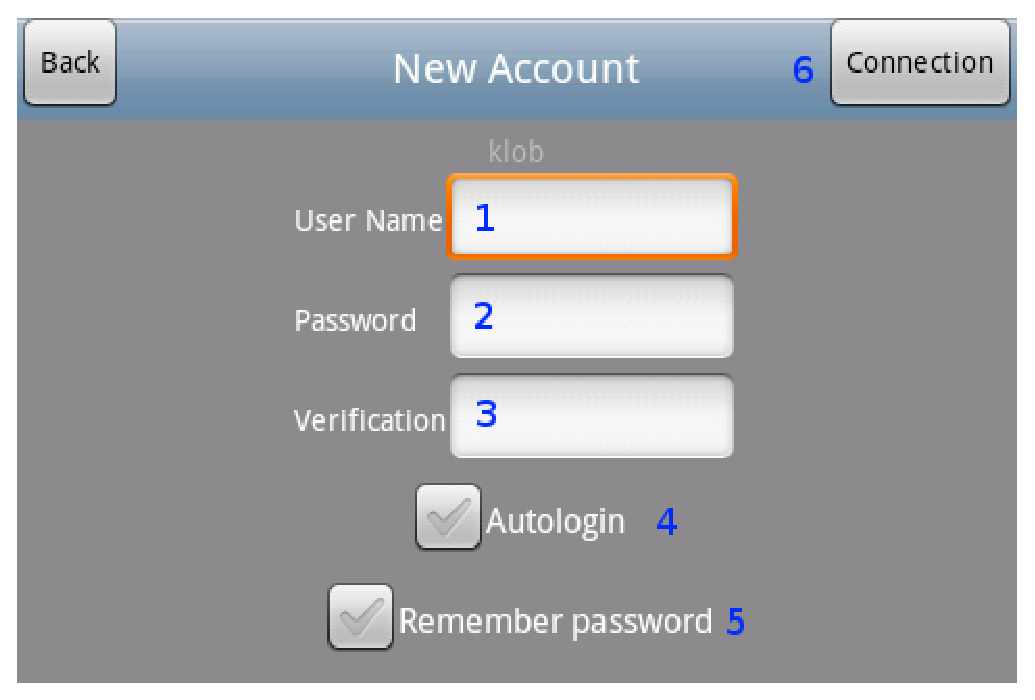
\includegraphics[scale=0.7]{Manuel/Img/18.eps}
	\end{center}
	
	\subsubsection{Connexion}
		Une fois seulement l'étape précédente accomplie, vous pouvez passer par le
		menu de connexion. Dans ce dernier, il faut donner le couple
		nom d'utilisateur \textcolor{blue}{\textbf{1}}/mot de passe
		\textcolor{blue}{\textbf{2}}. Vous pouvez aussi choisir, dans le cas d'une
		identification correcte, la mémorisation de votre compte
		\textcolor{blue}{\textbf{3}}, c'est à dire un accès direct sans passer par le
		menu de connexion, ou la mémorisation unique de votre mot de passe
		\textcolor{blue}{\textbf{4}}. Enfin, il est toujours possible de créer un
		nouveau compte multijoueur \textcolor{blue}{\textbf{5}}. Là encore une
		vérification sur le serveur est faite lorsque vous choisissez la connexion
		\textcolor{blue}{\textbf{6}}.
		
		\begin{center}
			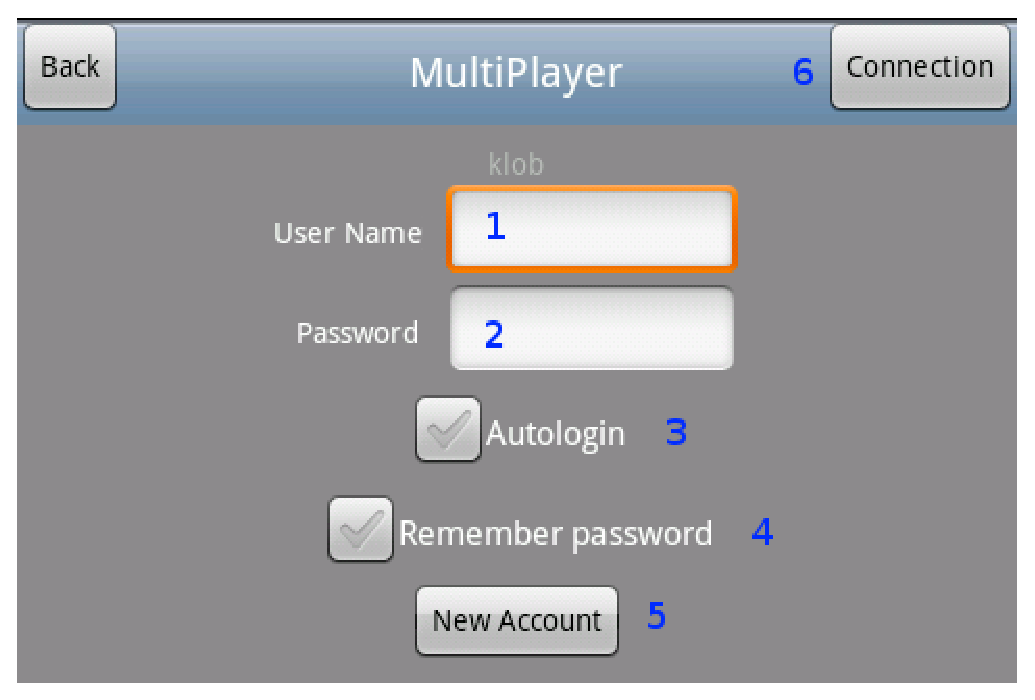
\includegraphics[scale=0.7]{Manuel/Img/17.eps}
		\end{center}
	
	\subsubsection{Accueil}
	L'accueil du mode multijoueur est composé d'un champ éditable, permettant le
	tri des parties en lignes \textcolor{blue}{\textbf{1}}, le rafraîchissement des
	parties \textcolor{blue}{\textbf{2}}, une liste déroulante cliquable de celles
	en cours \textcolor{blue}{\textbf{3}}, et enfin un accès au menu de création
	d'une nouvelle \textcolor{blue}{\textbf{4}}.
	
		
	\begin{center}
		\includegraphics[scale=0.6]{Manuel/Img/19.eps}
	\end{center}
	
	\subsubsection{Créer partie}
	La création multijoueur et semblable à celle en locale.
	Vous choisissez le type de partie
	\textcolor{blue}{\textbf{2}}, le nombre
	d'ennemis sur la carte \textcolor{blue}{\textbf{3}}, et le temps de jeu
	\textcolor{blue}{\textbf{4}}, et enfin grâce à un défilement de la galerie
	\textcolor{blue}{\textbf{1}}, la carte du jeu. Vous pourrez revenir au menu
	précédent \textcolor{blue}{\textbf{5}} ou vous validerez
	\textcolor{blue}{\textbf{6}} pour créer la partie.
	
	\begin{center}
		\includegraphics[scale=0.4]{Manuel/Img/16.eps}
	\end{center}

\subsection{Editeur de map \textcolor{red}{3} }
	
	\subsubsection{Création de map}
	Comme dans tout jeux d'arcade qui se respecte, vous avez la possibilité de
	créer vos niveaux via un éditeur. Vous n'avez qu'à donner le nom de la carte
	\textcolor{blue}{\textbf{1}} que vous souhaitez créer puis valider
	\textcolor{blue}{\textbf{2}}. La encore les doublons ne sont pas possibles.
	
	\begin{center}
			\includegraphics[scale=0.9]{Manuel/Img/10.eps}
	\end{center}
	
	
\subsubsection{Charger map}
	Après avoir enregistré une carte que vous ou un autre compte local aurait crée,
	il vous est possible de l'éditer et de l'enregistrer et ce en la choisissant
	\textcolor{blue}{\textbf{1}} parmi toutes les cartes crées et de valider
	\textcolor{blue}{\textbf{2}}. 
	
	\begin{center}
		\includegraphics[scale=0.9]{Manuel/Img/14.eps}
	\end{center}
	

\subsection{Options \textcolor{red}{4}}
	Le menu d'option est à votre disposition pour régler vos paramètre systèmes
	mais aussi le profils d'utilisateur local et multijoueur.
	
	\subsubsection{Réglage sytème}
	Ce type de réglage a été conçu pour ajuster le son
	\textcolor{blue}{\textbf{1}} à votre convenance mais aussi choisir la langue
	\textcolor{blue}{\textbf{2}} utilisée dans votre jeu. Sont à votre disposition
	le français mais aussi l'anglais.
	
	\begin{center}
		\includegraphics[scale=0.8]{Manuel/Img/4.eps}
	\end{center}
	
	\subsubsection{Gestionnaire profil}
		Dans ce menu, vous avez accès à l'édition de vos profils locaux et
		multijoueurs. Une fois vos modifications accomplies n'oubliez pas de les
		valider en cliquant sur le bouton Ok situé en haut à droite de votre fenêtre.
		\paragraph{Local\\}
		Il vous est ici possible de changer le pseudonyme \textcolor{blue}{\textbf{1}}
		de votre compte local en cours, mais aussi de choisir la couleur de votre
		personnage \textcolor{blue}{\textbf{2}}, toujours pour les parties locales.
		\begin{center}
				\includegraphics[scale=0.8]{Manuel/Img/5.eps}
			\end{center}
		
		\paragraph{Multijoueur\\}
		Une fois un compte multijoueur crée sur le serveur, cet onglet vous donnera la
		possiblité d'éditer \textcolor{blue}{\textbf{1}} le nom d'utilisateur et le mot de passe mais
		aussi de changer de compte multijoueur \textcolor{blue}{\textbf{2}}. Les
		paramètres d'accès comme la connexion automatique
		\textcolor{blue}{\textbf{3}} ou la sauvegarde du mot de passe
		\textcolor{blue}{\textbf{4}} sont ici configurables dès lors que le couple
		nom d'utilisateur/mot de passe sera renseigné et valide.
		
		\begin{center}
				\includegraphics[scale=0.8]{Manuel/Img/6.eps}
		\end{center}
		
		\newpage{}	
		\paragraph{Général\\}
		Grâce au menu déroulant \textcolor{blue}{\textbf{1}}, vous pouvez fixer le
		côté de l'écran où est positionné le menu de jeu, c'est à dire celui contenant
		le bouton pour posé une bombe pendant une partie, suivant si l'on est gaucher ou droitier. 
		
		\begin{center}
				\includegraphics[scale=0.8]{Manuel/Img/7.eps}
		\end{center}
			
			
	\paragraph{Choisir compte local \textcolor{red}{5}\\}
	Afin de permettre l'utilisation de l'application par plusieurs joueurs et donc
	comptes. Il vous est possible de les choisir grâce à une liste des comptes
	locaux. 
	\begin{center}
		\includegraphics[scale=0.6]{Manuel/Img/8.eps}
	\end{center}
	
	\newpage{}	

	\paragraph{Ajouter compte local \textcolor{red}{6}\\}
	Il est nécessaire comme au premier lancement, de renseigner un pseudonyme 
	\textcolor{blue}{\textbf{1}}. Dans ce cas là une vérification de disponibilité
	de votre pseudonyme est faite. Une fois valide vous
	revenez sur le menu d'accueil avec votre nouveau compte local sélectionné.
	\begin{center}
		\includegraphics[scale=0.6]{Manuel/Img/9.eps}
	\end{center}
	
\section{Jeu}
	Après avoir choisi vos préférences pour votre partie, celle-ci se lance.
	Pour déplacer votre joueur, il vous suffit d'effleurez l'écran de jeu dans le sens et la
	direction où vous souhaiter aller \textcolor{blue}{\textbf{1}} .	
	Sur le panneau de droite en appuyant sur le
	bouton prévu \textcolor{blue}{\textbf{2}}, vous posez des bombes.
	Le panneau du haut résume les informations de la partie. Le temps de jeu
	\textcolor{blue}{\textbf{3}} restant, et vos différents bonus. Ces derniers
	correspondent à la portée de vos bombes \textcolor{blue}{\textbf{4}}, le
	nombres de bombes que vous pouvez poser
	simultanément \textcolor{blue}{\textbf{5}}, la vitesse de déplacement de votre
	joueur \textcolor{blue}{\textbf{6}}, et votre compteur de vies
	\textcolor{blue}{\textbf{7}}.
	
	\begin{center}
		\includegraphics[scale=0.6]{Manuel/Img/21.eps}
	\end{center}
	
	\subsection{Pause\\}
	Lors d'une partie, vous pouvez la suspendre en appuyant sur le Menu
	\textcolor{orange}{\textbf{1}} en haut à gauche. Il vous est possible de
	reprendre la partie \textcolor{orange}{\textbf{2}}, accéder aux options de jeu
	\textcolor{orange}{\textbf{3}}, redémarrer la partie
	\textcolor{orange}{\textbf{4}}, ou tout simplement la quitter et revenir au
	menu \textcolor{orange}{\textbf{5}}. 
	
	\begin{center}
		\includegraphics[scale=0.8]{Manuel/Img/20.eps}
	\end{center}




	
\section{Edition de map}
	Une carte vierge s'offre à vous \textcolor{blue}{\textbf{1}}. Le choix des
	structures(destructibles ou non) \textcolor{blue}{\textbf{2}}, de la texture du
	sol \textcolor{blue}{\textbf{2'}} mais aussi le positionnement des joueurs
	\textcolor{blue}{\textbf{3}} vous est alors mis à disposition. Pour passer des
	structures aux textures du sol, utilisez l'interrupteur situé en haut à droite
	de l'écran \textcolor{blue}{\textbf{4}}. Vous pourrez ensuite choisir l'image
	que vous souhaitez dessiner. Remarquez qu'en slidant de haut en bas, les images
	défilent ainsi, et inversement. Ensuite vous avez juste à appuyer à l'emplacement où 
	vous désirez ajouter l'objet préalablement choisi. Il est aussi possible de rester appuyer sur l'écran tout en
	glissant, l'image choisit est alors appliquée sur toutes les cases survolées.
	
	
	\begin{center}
		\includegraphics[scale=0.9]{Manuel/Img/11.eps}
	\end{center}
	
	\subsection{Enregistrement map\\}
	Une fois votre carte achevée ou non, vous pouvez accéder au menu d'option
	via le bouton Menu \textcolor{orange}{\textbf{1}} . Ce dernier vous propose
	alors de retourner sur l'éditeur \textcolor{orange}{\textbf{2}}, d'enregistrer votre
	carte et quitter \textcolor{orange}{\textbf{3}}, de remettre à zéro votre carte
	\textcolor{orange}{\textbf{4}}, et enfin quitter sans enregistrer
	\textcolor{orange}{\textbf{5}}. 
	
	\begin{center}
		\includegraphics[scale=0.9]{Manuel/Img/13.eps}
	\end{center}
	
	

	

\chapter{Discussion}

	\section{Difficultés}
	Lors du développement de l'application, nous avons rencontré de nombreuse difficultés.
	
	Tout d'abord la principale difficulté était le fait que nous devions développer une application mobile, ce qui nous limitait au niveau des ressources disponible. De plus nous avions jamais développé une application sous \gls{android} et \gls{ios}.
	
	\subsection{Android}
		La difficulte que nous avons eu durant le développement de l'application sous \gls{android} était d'implémenter le multi-touch pour que le joueur puisse à la fois bouger et poser une bombe.
	
	\subsection{iOS}
		% TODO: Mettre garbage collector dans le glossaire.
		Pour \gls{ios}, la principale difficulté a été d'apprendre l'\gls{objective-c} car c'est un langage qui était totalement nouveau, malgrès le fait qu'il est relativement similaire au \gls{java}. De plus, ce dernier ne posséde pas de garbage collector pour \gls{ios}, ce qui nous a obligé de gérer la mémoire manuellement, ce que nous avions jamais fait.
	
	\subsection{Serveur}
		% TODO: Mettre servlet dans le glossaire
		Enfin, pour le serveur, nous avons eu des problèmes los du déploiment local du serveur d'application et aussi des servlets car nous avions jamais réalisé ces derniers. La communication entre le serveur d'application est la base de données, nous a aussi posé des problèmes.


\section{Problèmes}
	
	\subsection{Mobile}
		Le problème majeur a été de tester notre appliction. Tout d'abord au début du projet, nous ne possédions pas de téléphone sous \gls{android}. Ensuite au niveau d'\gls{ios}, nous avons pas pu tester notre application sur un \gls{iphone} car il faut obligatoirement posséder un compte au centre de développement d'Apple (ce dernier coût 99\$ par an), ce que nous pouvions pas nous payer.
		
		% TODO: Vérifier le terme "nouveau langage"
		L'autre problème était de savoir si nous allons utiliser \gls{opengl_es} pour le développement de l'application. Ce qui nous aurait permi d'avoir un code portable donc il aurait été compatible pour \gls{android} et \gls{ios}. Grâce à cette portabilité, cela nous aurait permi de développer qu'un code source et donc ça nous aurait fait gagné du temps en revanche il aurait encore fallu apprendre un nouveau langage.

	
	\subsection{Serveur}
		% TODO: Vérifier cette partie (voir avec Ludo)
		Au niveau du serveur, nous avons eu un problème de pour déployer ce dernier sur internet.

	
\section{Améliorations}
	% TODO: Disponible en annexe ?
	Le développement de ce type de jeu permet d'ajouter un grand nombres d'améliorations. Notamment la gestion des bonus et des malus qui rendent le jeu beaucoup plus amusant et qui est disponible en annexe. Il y a aussi la gestion de différents types de parties, comme: la capture de drapeau,  les parties en équipe, etc. Nous aurions aussi pu ajouter un mode histoire pour les plus gourmands et pour rendre le jeu plus attractif. Puis une des améliorations les plus importantes, est l'ajout du mode multijoueur en WI-FI au niveau national (puis international ?) car ce dernier n'existe pas encore sur mobile et aurait très bien pu révolutionner le jeu bomberman sur mobile.


\subsection{Serveur}
	\begin{itemize}
		\item{Pooling}
		\item{Session}
	\end{itemize}



	
			
\chapter{Conclusion}

	L’application que nous avons réalisée est fonctionnelle et respecte les contraintes de fonctionnalités minimales imposées. Malheureusement nous n'avons pas eu le temps de developper le mode mutlijoueur  qui aurait été très enrichissant. Mais nous avons quand même implémenté la partie réseau qui  nous permettra dans un futur proche de pouvoir continuer à developper ce dernier dans le but de partager notre application sur l'AppleStore et l'AndroidMarket.

Toutes les fonctionnalités implémentées fonctionnent parfaitement malgres que durant le développement et les tests que nous avons réalisé, nous avons décelé quelques bogues minimes qui ont été corrigés au jour d’aujourd’hui.

Les langages que nous avons utilisés nous ont permis d'étoffer notre maitrise de la programmation objet et de découvrir le developpement mobile.
L'analyse du projet quand à elle s’est avéré suffisante et efficace car l’application fonctionne et que l’implémentation d’une multitude de fonctionnalités est envisageable.\\

Nous avons du développer cette application à quatre. Cela a été un handicap car nous disposions d’un temps limité et que le développement de deux applications comme celle-ci demande une vraie équipe de projet composée de plusieurs membres. Heureusement, gâce à notre organisation, à la bonne entente et la bonne communication au sein du groupe, nous avons pu travailler de manière efficace. Mais cela nous a aussi permis de partager nous connaissances et de nous entraider tout au long de ce projet.

\end{document}
